%% Dokumentklasse KOMA-Script Report
\documentclass[paper=a4, 12pt]{scrreprt}
%% Encoding UTF8
\usepackage[utf8]{inputenc}
%% 8 Bit Aufloesung der Buchstaben
\usepackage[T1]{fontenc}
%% Seitenraender
\usepackage[scale=0.85]{geometry}
%% Spracheinstellungen
\usepackage[english, naustrian]{babel} % your native language must be the last one!!
%% erweiterte Farbenpalette
\usepackage[dvipsnames]{xcolor}
%% Abbildungen
\usepackage{float}
\usepackage{adjustbox}
%% Tabellen (erweitert)
\usepackage{tabularx}
%% TikZ + Circuit-TikZ (fuer Schaltungen)
\usepackage[europeanresistors, europeaninductors]{circuitikz}
%% Nuetzliche TikZ Libraries
\usetikzlibrary{arrows, automata, positioning}
%% mathematik
\usepackage{amsmath, amssymb}
%\usepackage{mathtools}	
%% pdf-einbindung
\usepackage{pdfpages}
%% scource-code einbindung
\usepackage{listings} %scrhack vermeidet Umschaltung auf KOMA Floats..
\usepackage{courier}
%% euro-symbol
\usepackage{eurosym}
%% landcsape-seiten ermöglichen
\usepackage{lscape}

%% Diplomarbeits-Format
\usepackage{srdpdipa}

%% Abkuerzungsverzeichnis
\usepackage[]{acronym}

%% Todos
\usepackage[]{todonotes}

%% Ganttdiagramme
\usepackage{pgfgantt}

%% Subfigures
\usepackage[lofdepth]{subfig}

\lstdefinestyle{customc}{
	belowcaptionskip=1\baselineskip,
	breaklines=true,
	frame=L,
	xleftmargin=\parindent,
	language=C,
	showstringspaces=false,
	basicstyle=\footnotesize\ttfamily,
	keywordstyle=\bfseries\color{green!40!black},
	commentstyle=\itshape\color{purple!40!black},
	identifierstyle=\color{blue},
	stringstyle=\color{orange},
}


\lstset{escapechar=@,style=customc}

%% definitionen =====================================%%
\dataSchool{HTBLuVA St. Pölten}
\dataDepartment{Höhere Lehranstalt für Elektronik und Technische Informatik}
\dataSubdepartment{Ausbildungsschwerpunkte Embedded Systems}
\dataSession{2019/20}

\title{Universeller hochdynamischer LED-Treiber}
\author{Florian Hintermeier \and Dominik Gansch}
\date{\today}
\place{St. P\"olten}
\professor{Dipl.-Ing. Josef Radlbauer}
%%====================================================%%

% Hyperlinks im Dokument
\usepackage[colorlinks=true,
    linkcolor=black,
    citecolor=green,
    bookmarks=true,
    urlcolor=black,
    bookmarksopen=true]{hyperref}

\begin{document}

\frontmatter

%% titelseite ==========================================%%
\maketitle
%%======================================================%%

%% komplett leere seite ================================%%
\newpage\null\thispagestyle{empty}\newpage
%%======================================================%%

%% eidesstattliche erklärung ===========================%%
\includepdf[pages=-]{form/eid.pdf}
%%======================================================%%

%% danksagungen=========================================%%
\begin{acknowledgements}
	\begin{center}
    Wir danken allen die die uns mit Ratschlägen und Ideen bei unserer Arbeit geholfen haben. Besonderer Dank fällt an Dipl.-Ing. Josef Radlbauer, der uns als Betreuer unserer Diplomarbeit immer wieder mit Ratschlägen und Ideen zur Seite Stand. Wir danken auch Dipl.-Ing. Markus Tillich für Tipps und Ratschläge beim Schaltungsdesign des Schaltwandlers. Besonderer Dank fällt auch an Ing. Rudolf Janeczek BEd MSc, der für uns den Kontakt mit der Firma ZKW aufgebaut hat, die uns mit der Idee für die Diplomarbeit betraut machten. Den Vertreten der Firma ZKW, Matthäus Artmann und Daniel Seitl, welche unsere Hauptansprechpartner waren, möchten wir besonders danken. 
	\end{center}
\end{acknowledgements}
%% Für Diplomarbeit hinzufügen
%%======================================================%%

%% dokumentation (deutsch/englisch) ====================%%
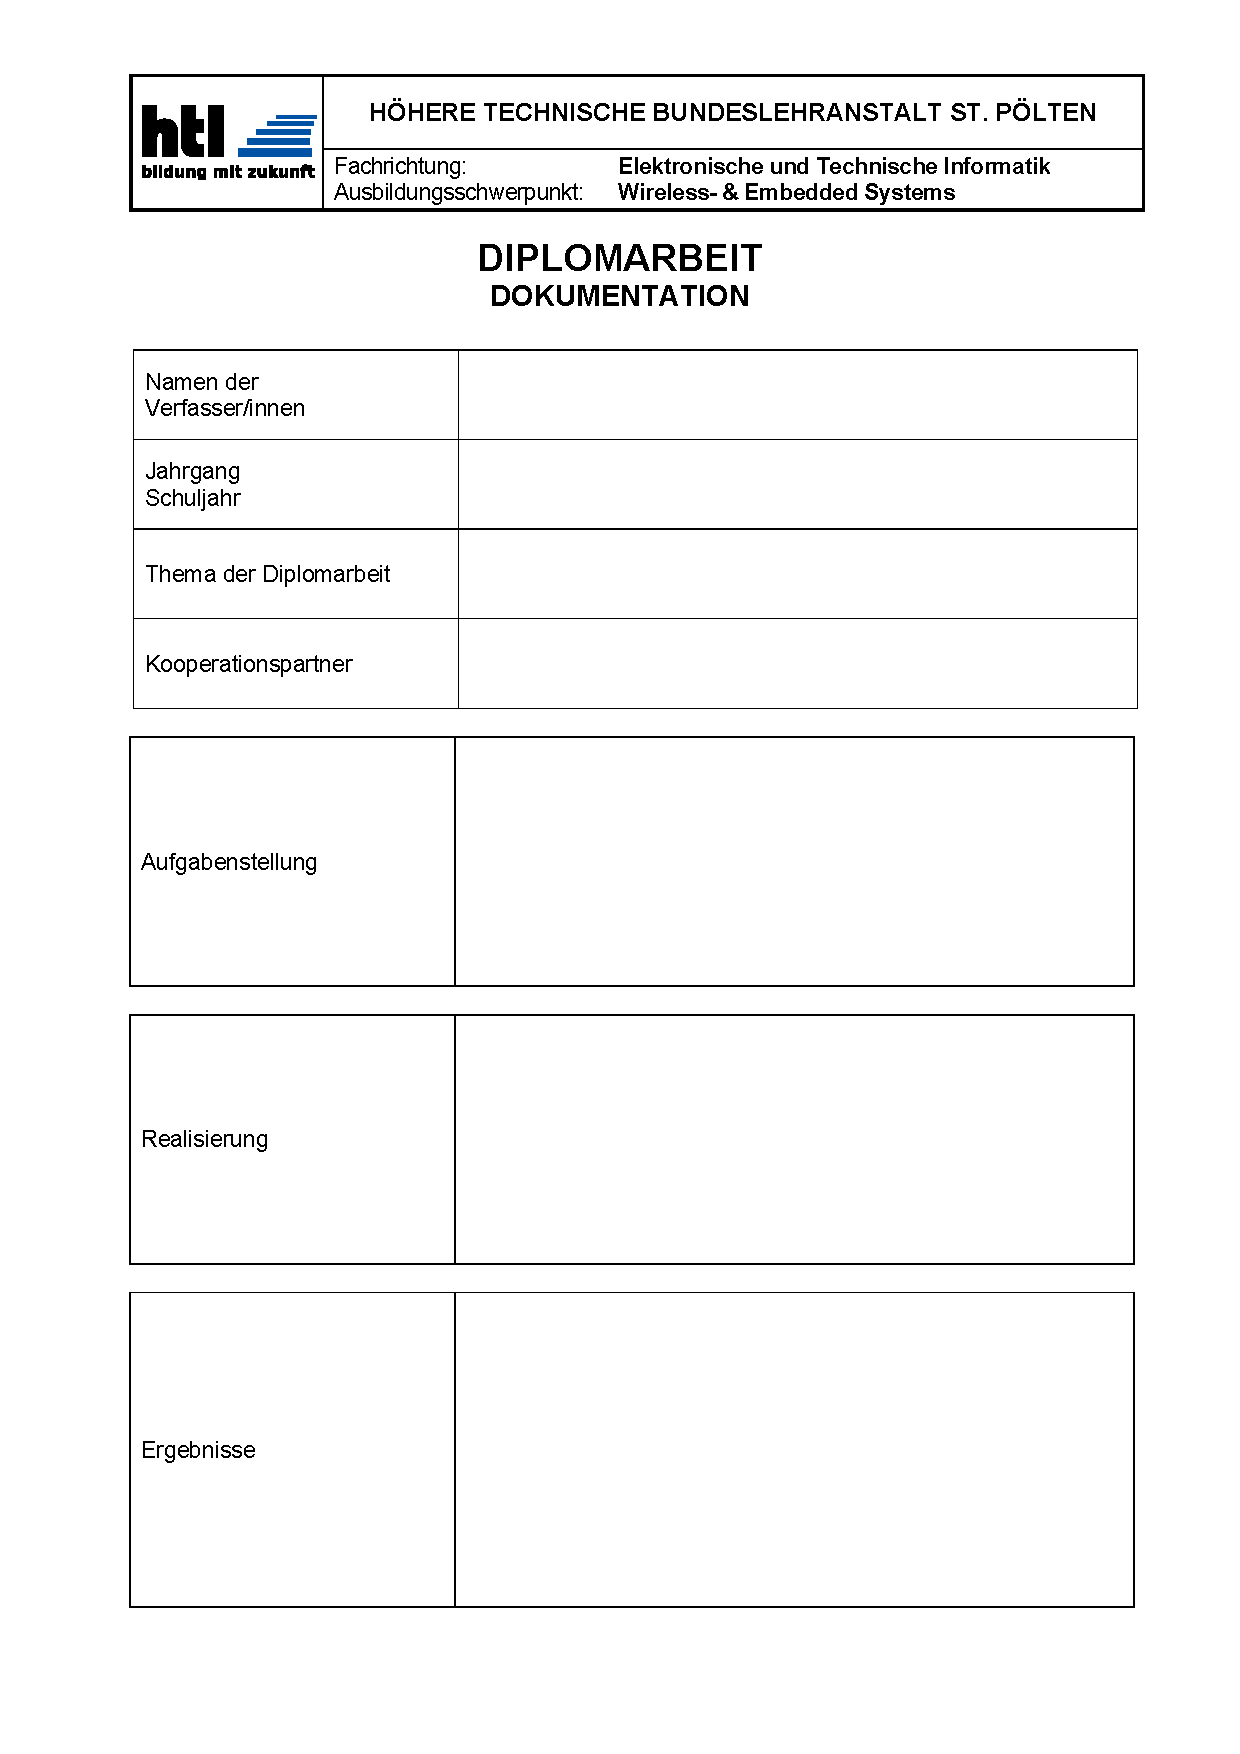
\includepdf[pages=-]{form/dokumentation-de.pdf}
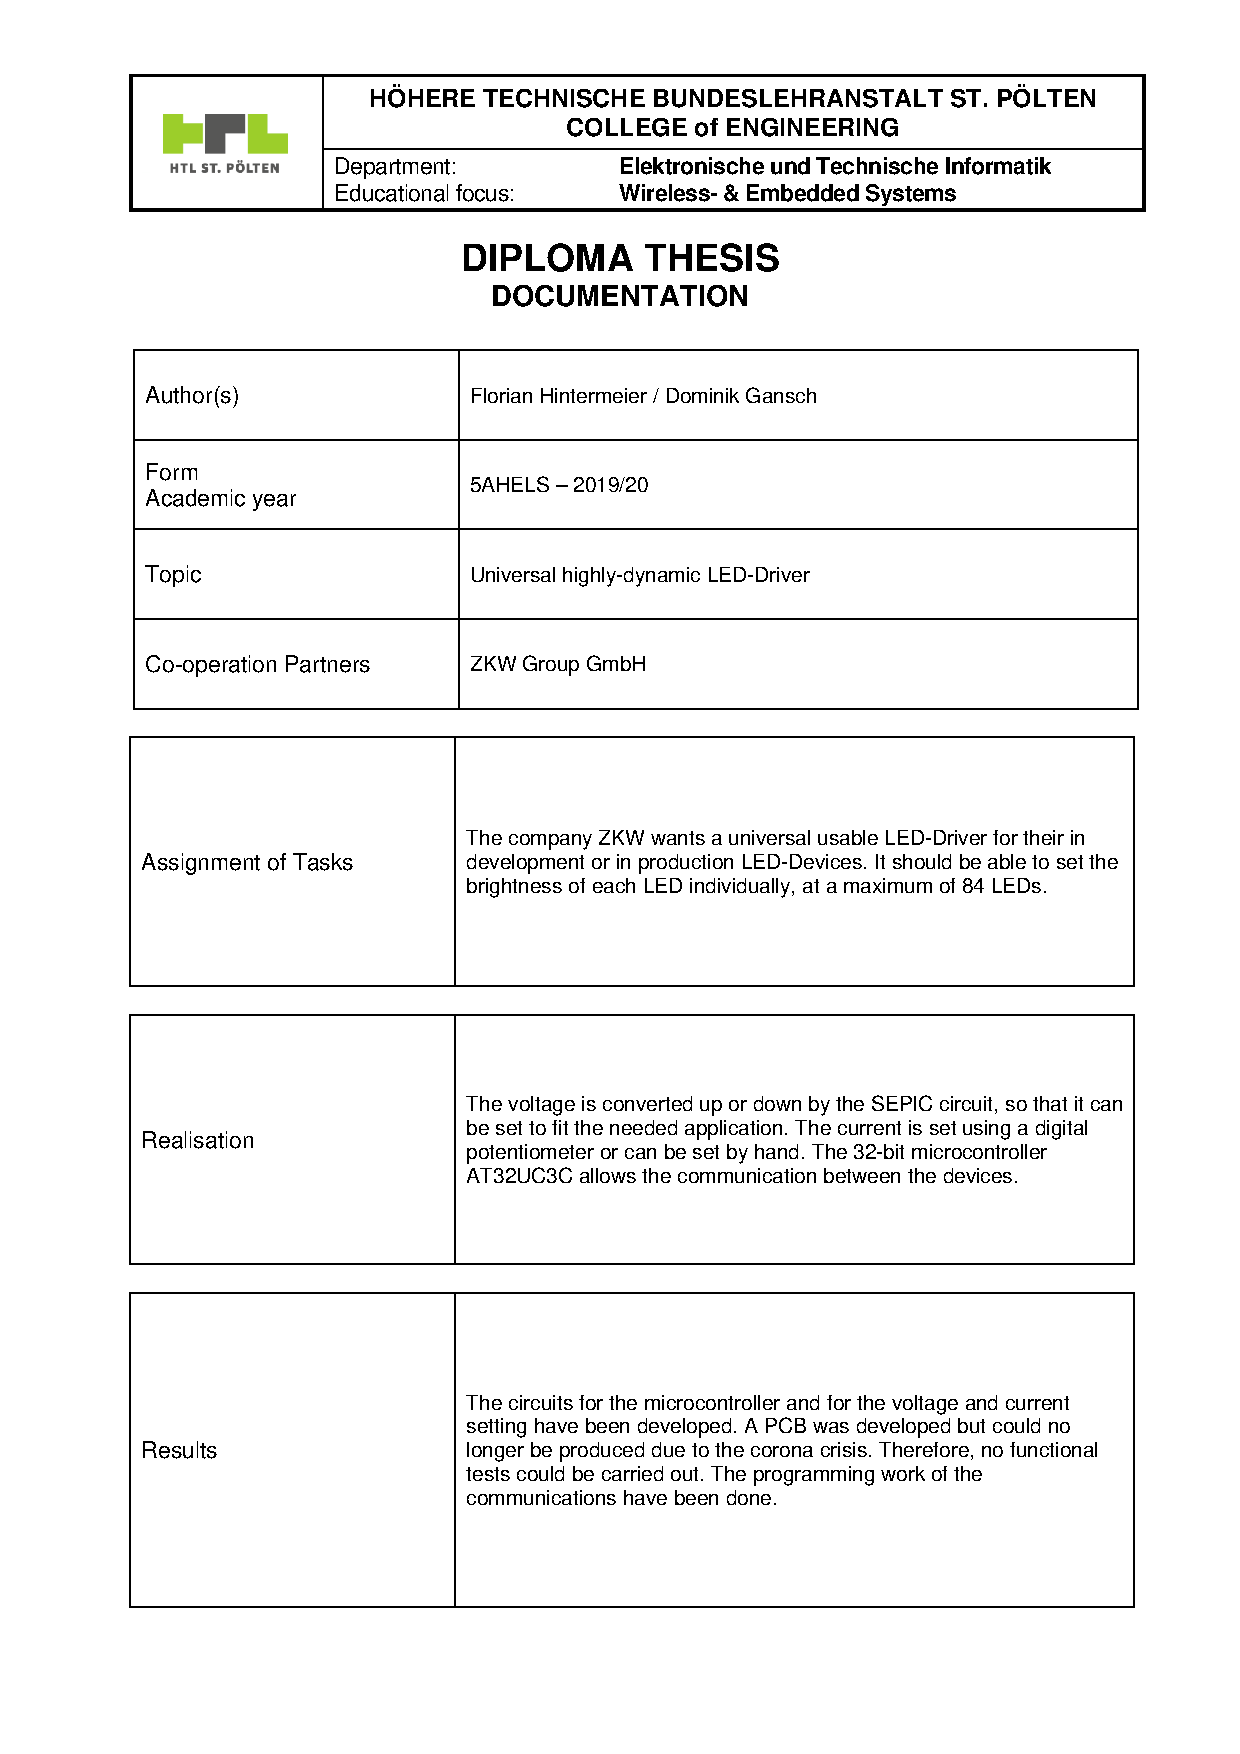
\includepdf[pages=-]{form/dokumentation-en.pdf}
%%======================================================%%

%% inhaltsverzeichnis ==================================%%
\tableofcontents
%%======================================================%%

%% HAUPTTEIL ===========================================%%
\responsible{Florian Hintermeier, Dominik Gansch}
\mainmatter

\chapter{Einleitung}\hfill \break
    Die Firma ZKW möchte für zahlreiche in Entwicklung und bereits in Produktion befindliche LED Einheiten einen universell einsetzbaren LED Treiber mit linear einstellbarem Strom. Dabei soll jede einzelne LED, maximal 84, individuell in ihrer Helligkeit eingestellt werden können.
    
	\begin{adjustbox}{center,caption={Blockschaltbild von ZKW},label={ZKW-Blockschaltbild},nofloat=figure,vspace=\bigskipamount}
	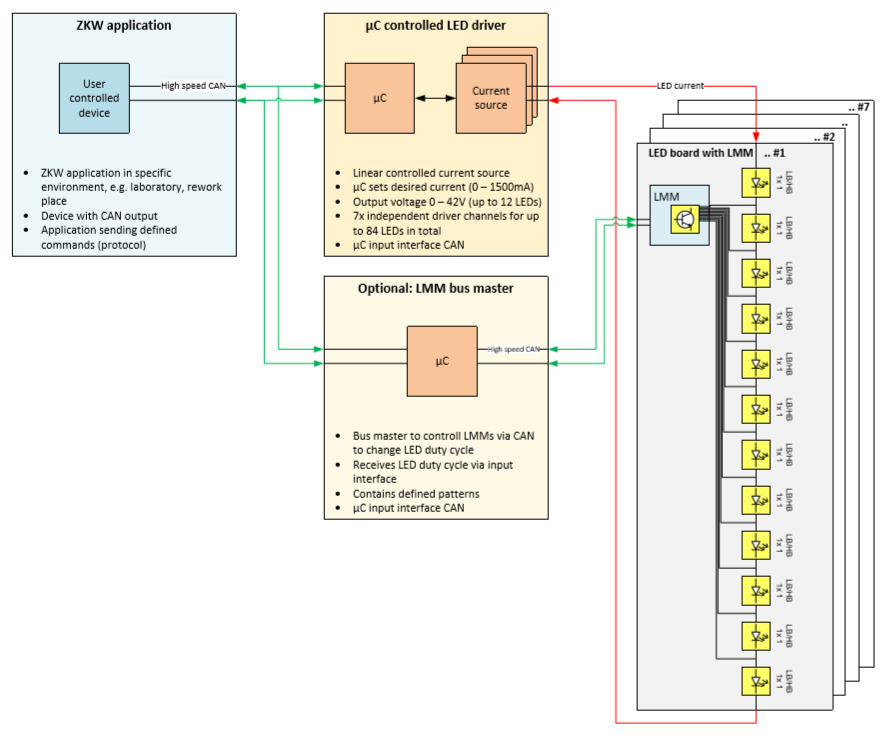
\includegraphics[width=15cm]{img/ZKW_Blockschaltbild.PNG}
	\end{adjustbox}

	Das Ziel liegt darin, eine geeignete Schaltung zu entwickeln, um den von ZKW gegebenen Anforderungen zu entsprechen. Zu sehen sind diese in Abbildung 1.1.
	
	Diese Angaben sind:
	\begin{itemize}
		\item{Eingangsspannung zwischen 10 und 15 Volt}
		\item{Einstellbare Ausgangsspannung bis 42 Volt}
		\item{Einstellbaren Ausgangsstrom zwischen 0 und 1500mA}
		\item{Mikrocontroller kommunikation über High-Speed-CAN}
		\item{Unterstützung für maximal 7 LED Boards mit gesamt maximal 84 LEDs}
	\end{itemize}
	
	\section{Meilensteine}\hfill \break
	\begin{adjustbox}{center,nofloat=figure,vspace=\bigskipamount}
	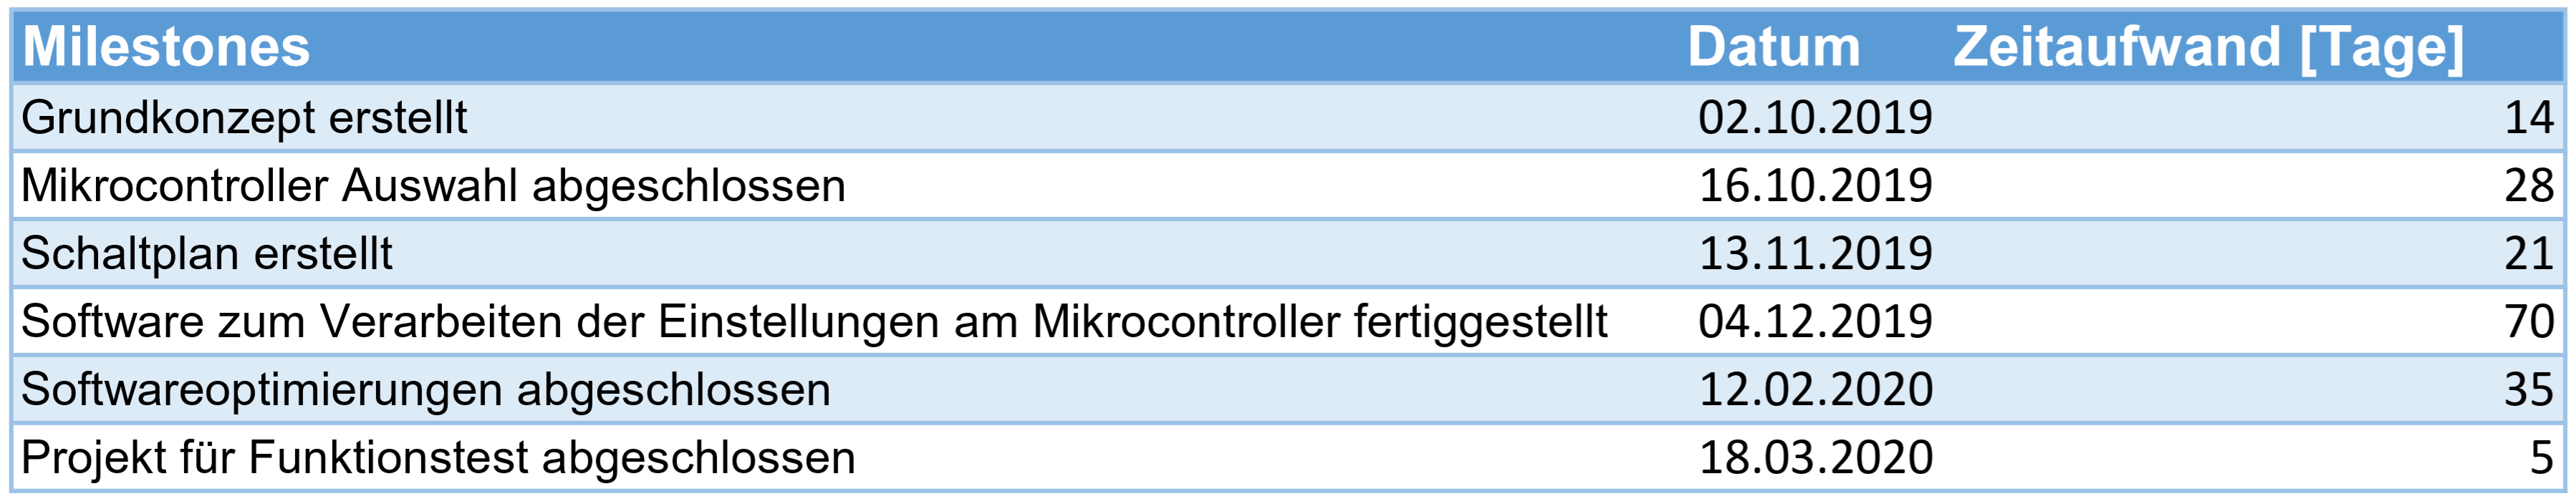
\includegraphics[width=\textwidth]{img/meilensteine.PNG}
	\end{adjustbox}
	
	\section{Projektplan}\hfill \break
	\begin{adjustbox}{center,nofloat=figure,vspace=\bigskipamount}
		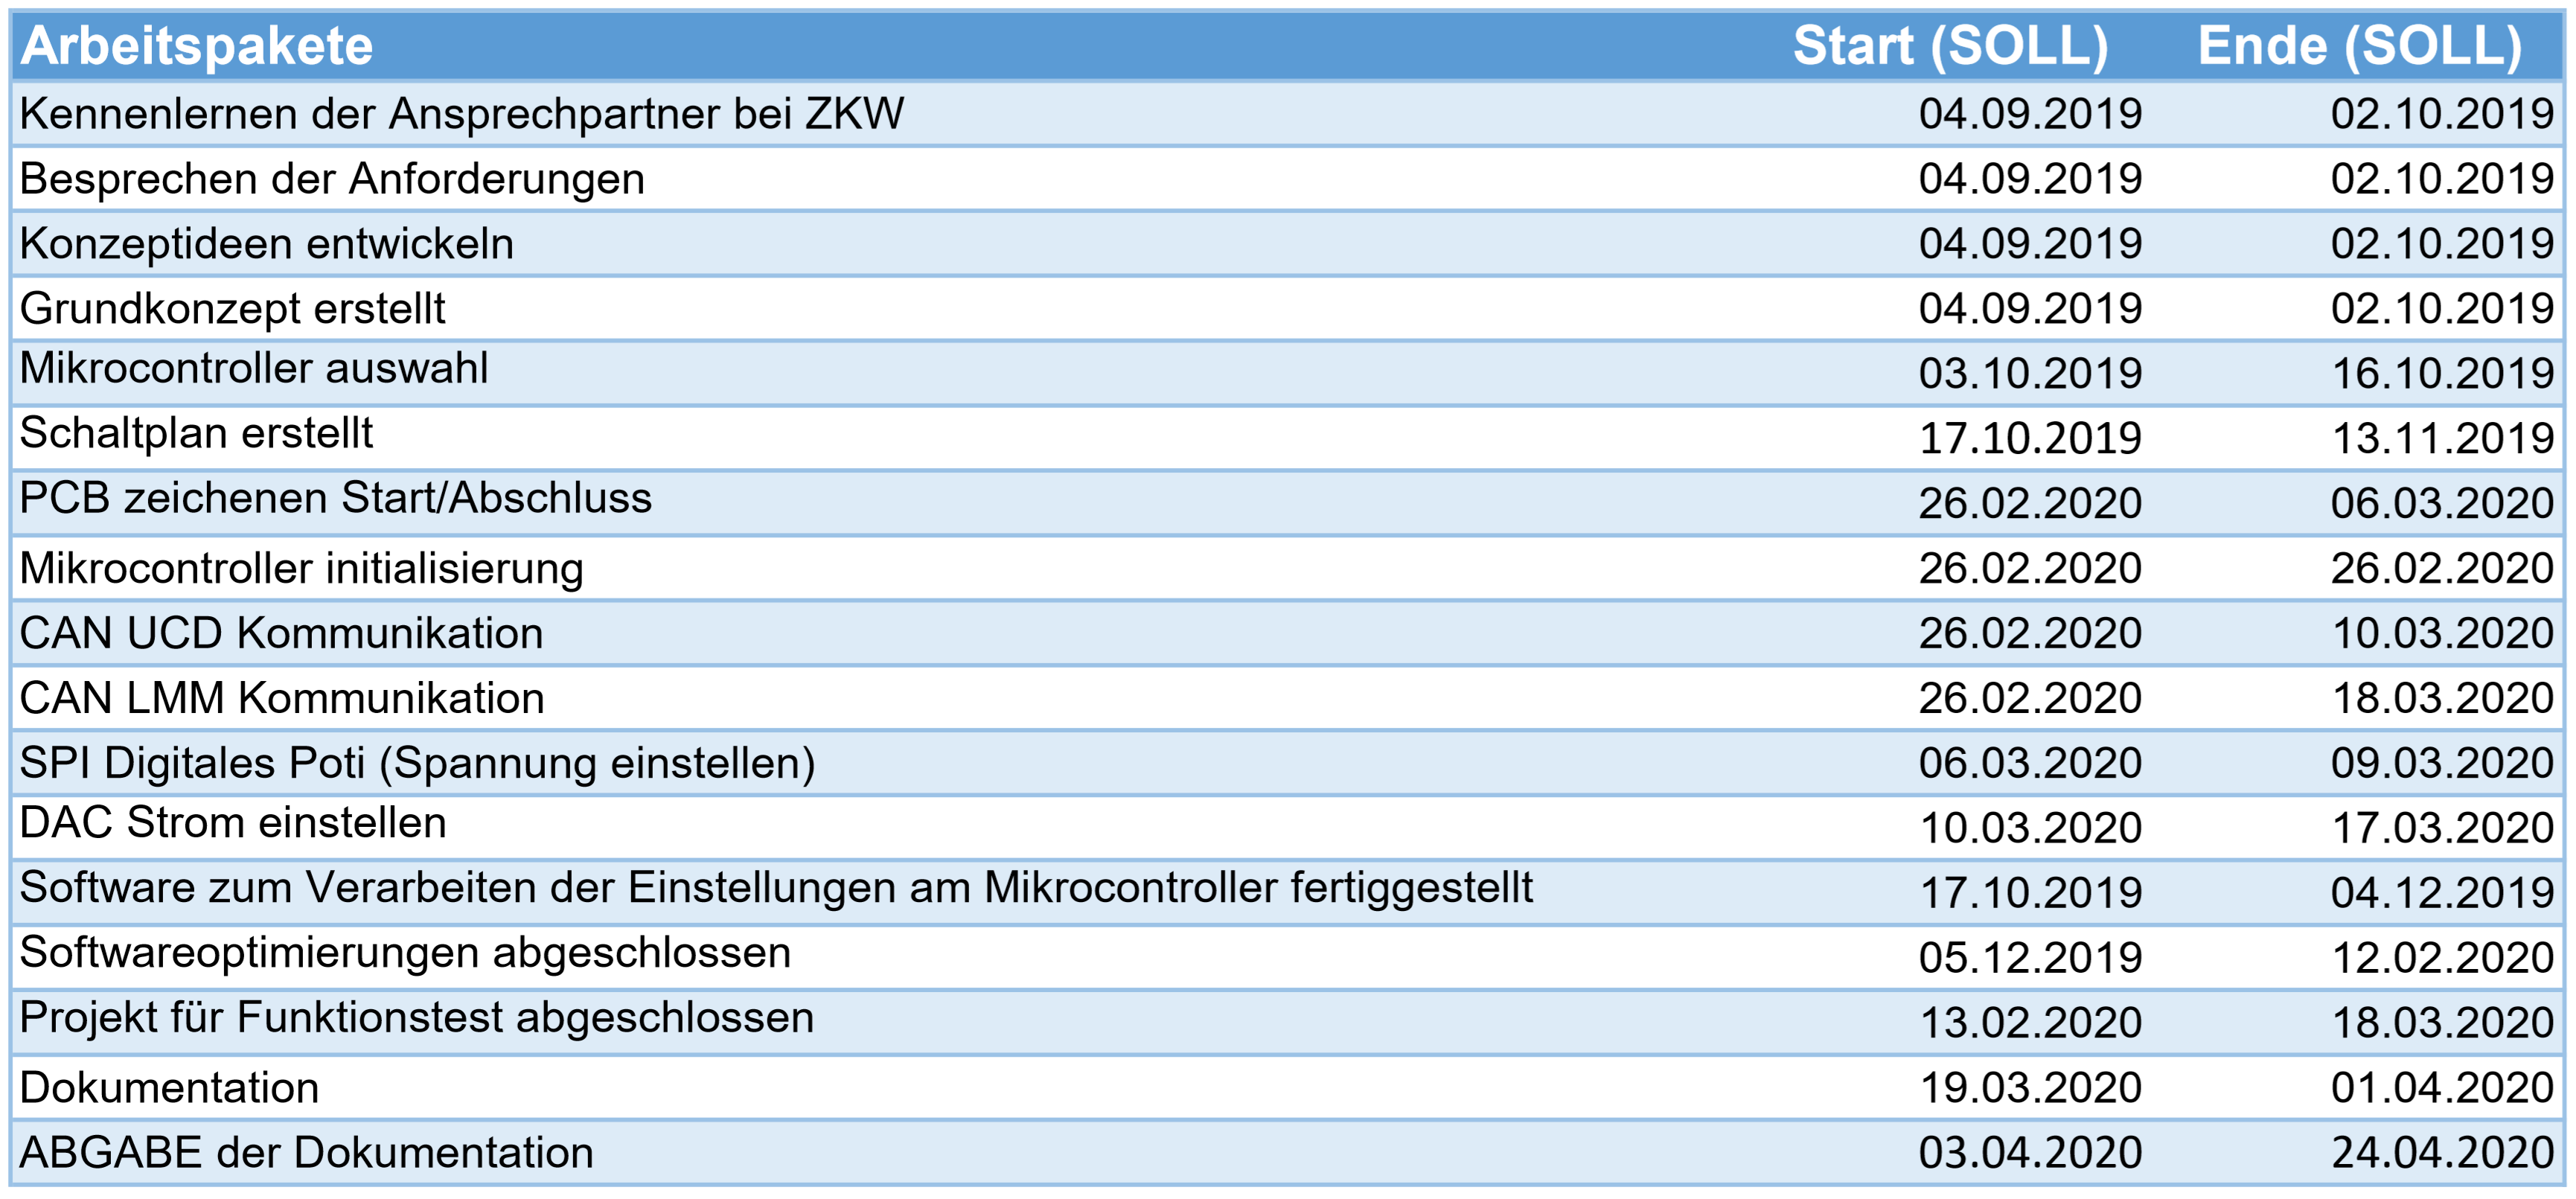
\includegraphics[width=\textwidth]{img/plan.PNG}
	\end{adjustbox}
	

\chapter{Individuelle Zielsetzung}\hfill \break
    \section{Hardware}    	\hfill \break
    	\subsection{Analogteil}\hfill \break
        Dieser Teil wird von Florian Hintermeier entwickelt. Der Analogteil enthält die Schaltung um die angeforderten Spannungen und Ströme erzeugen zu können, die von einem Mikrocontroller eingestellt werden sollen. Die Einstellungen werden von dem Mikrocontroller vom Digitalteil über den DAC eingestellt.
        
        \subsection{Digitalteil}\hfill \break
        Dieser Teil wird von Dominik Gansch entwickelt. Der Digitalteil dient als zentrale Steuerungseinheit. Das Kernstück des Digitalteils besteht aus dem Mikrocontroller welcher über CAN-Bus Befehle, von der ZKW-Application, bestimmte Kommandos erhält. Mithilfe der  CAN-Befehle werden vom Mikrocontrollerinternen DAC die Stromregelungsreferenz eingestellt bzw. sendet der Mikrocontroller die entsprechenden Lichtbilder an die LMMs.
          % Die CAN-Befehle kann man in zwei Gruppen einteilen, in Befehle für die LMMs und in Stromregelungsbefehle. Für jedes LMM-Kommando gibt es im Mikrocontroller eine entsprechende Lichtbild-Ablauf-Tabelle, diese Daten der Tabelle werden, nach erhalten des dafür entsprechenden Befehls, laufend zu den LMMs gesendet und von diesen umgesetzt, bis der Lichbild-Ablauf abgeschlossen ist. Befehle für die Stromregelung werden mithilfe des internen DACs in einen Spannungsreferenzwert für die Stromregelung umgesetzt. %
        \subsection{PCB-Entwicklung}\hfill \break
        Das printed-circuit-board wird von Dominik Gansch designed. Anforderungen sind ein größentechnisch praktikables Design, welches aber keine Einschränkung in der Handhabung der Hardware bietet. Das heißt es wird auf Benutzerfreundlichkeit beim Design geachtet (Massebügel für Messungen, zusätzliche Lötpads für Tiefpasskondensatoren, usw.) ohne jedoch technische Nachteile hervorzurufen.
        \newpage
   \section{Software}\hfill \break
   		\subsection{Initialisierungen}\hfill \break
   		Dieses Teilgebiet der Softwareentwicklung wird von Florian Hintermeier umgesetzt. Es beschränkt sich auf die Initialisierung der Internen, sowohl auch der Peripherie Funktionalitäten des Mikrocontrollers.
   		\subsection{Controller Area Network}\hfill \break
   		Dieses Gebiet wird ebenfalls von Florian Hintermeier entwickelt. Es handelt sich hierbei um die Kommunikation zwischen User Controlled Device von ZKW mit dem LED-Treiber und des weiteren um die Kommunikation zwischen Treiber und LED Matrix Manager.
   		Die Kommunikation zum UCD stellt die Grundeinstellungen des Treibers zur Verfügung und diese werden dann umgesetzt und an den LMM weitergegeben.
   		\subsection{Serial Peripheral Interface}\hfill \break
    	Die SPI kommunikation zwischen Mikrocontroller und Digitalen-Potentiometer wird von Dominik Gansch abgehandelt. Mithilfe des Digitalen-Potentiometers wird die Ausgangsspannung des Schaltwandlers eingestellt. Das Potentiometer wird in der Spannungsregelung, als Spannungsteiler der Regelschleife des Schaltwandlers, verwendet.
    	\subsection{ADC/DAC Einstellungen}\hfill \break
    	Die Programmierung der analogen Hardware des Mikrocontrollers (ADC,DAC) wird von Dominik Gansch umgesetzt. Der ADC misst an einen Shunt-Widerstand die aktuelle Strombelastung am Ausgang des Schaltwandlers. Eingestellt wird der maximale Ausgangsstrom über eine Analogschaltung welche mithilfe des DAC gesteuert wird.
    	Mit dieser Methode der Stromeinstellung und Strommessung wird der Ausgangsstrom des Schaltwandlers, über die programmierte Software, geregelt.

\chapter{Grundlagen und Methoden}\hfill \break
	\section{Verwendete Software}\hfill \break
	Die hier aufgeführte und kurz erklärte Software wurde für die Erreichung der Ziele in diesem Projekt verwendet.
	
	\paragraph{LTSpice}\hfill \break
	LTspice ist eine kostenlose Software des ehemaligen Halbleiterherstellers Linear Technology (seit 2017: Analog Devices) zur Schaltungssimulation. Es basiert auf SPICE, ist dazu kompatibel und besonders zur Simulation von Schaltnetzteilen geeignet. Entwickelt und gepflegt wird es von Mike Engelhardt.\footnote{https://de.wikipedia.org/wiki/LTspice}
	\paragraph{Draw.io}\hfill \break
	Draw.io stellt sich als ein technisch anspruchsvolles Diagramm-Tool vor, das im Browser arbeitet und Modellierungssprachen wie UML, ERM und BTPM unterstützt. Die Standard-Version ist kostenlos.\footnote{https://www.tecchannel.de/a/draw-io-kostenloses-diagramm-tool-fuer-den-browser,2078028}
	\paragraph{Altium Designer 19}\hfill \break
	Eines der Hauptziele von Altium ist es, eine integrierte Entwicklungslösung zur Elektronikentwicklung anzubieten.
	Altium Designer beinhaltet die Schaltbildeingabe, einen PCB Layout Editor mit Integritätsanalyse sowie eine auf SPICE-Modellen gestützte Schaltungssimulation.\footnote{https://de.wikipedia.org/wiki/Altium\_Designer}\\
	In diesem Projekt wurde es dazu verwendet, um die Schaltungen zu zeichnen und das PCB damit zu erstellen.
	\paragraph{TeXstudio}\hfill \break
	TeXstudio ist ein LaTeX-Editor für Windows, Linux, BSD und (Mac) OS X. Er ist open source und basiert auf Texmaker. Wie andere bekannten LaTeX-Editoren bietet auch er die grundlegende Unterstützung beim Einfügen von LaTeX-Befehlen, Syntax-Hervorhebung, eine integrierte Vorschaufunktion und eine Projektfunktion.\footnote{https://latex.tugraz.at/programme/texstudio}
	\paragraph{MiKTEX}\hfill \break
	MiKTEX ist die benötigte erweiterung für TeXstudio um aus dem LaTeX-Syntax ein PDF erstellen zu können. Es ist sozusagen der Übersetzer von tex zu PDF. \newpage
	\paragraph{Atmel Studio}\hfill \break
	Das Atmel Studio (vor Version 6: "AVR Studio") ist eine kostenlose Entwicklungsumgebung (IDE) für die Programmierung der AVR-Mikrocontroller und ARM-Mikrocontroller (ab Version 6) von Atmel. Sie basiert ab Version 5 auf der Visual Studio Shell von Microsoft und besteht aus einer Projektverwaltung, einem Editor, einem Debugger und Werkzeugen zum Beschreiben der Mikrocontroller.\footnote{https://www.mikrocontroller.net/articles/Atmel\_Studio}
	\paragraph{GeoGebra}\hfill \break
	GeoGebra ist eine kostenlose dynamische Mathematiksoftware für SchülerInnen und LehrerInnen aller Altersstufen. Sie verbindet Geometrie, Algebra, Tabellen, Zeichnungen, Statistik und Analysis in einem einfach zu bedienenden Softwarepaket.\footnote{https://www.geogebra.org/about?lang=de}
	\paragraph{CanvasJS}\hfill \break
	CanvasJS ist eine leicht zu verstehende Diagrammerstellungs-Bibliothek auf Basis von Javascript, die dynamische Diagramme als Vektorgrafiken oder als HTML Elemente erzeugen kann. Es wurde verwendet um Diagramme, die zur Veranschaulichung etwaiger Berechnungen dienen, herzustellen.
	\newpage
	
	\section{Basis des Analogteils}\hfill \break
	Die Basis des Analogteils bildet eine SEPIC Schaltung für die Erzeugung der gewünschten Ausgangsspannung, das Funktionsprinzip davon wird unten beschrieben. Einen weiteren Teil bildet allerdings die Stromquelle, mit der man den maximalen Ausgangsstrom einstellen kann. Es ist möglich, diesen mittels Mikrocontroller oder Potentiometer einzustellen.
	\paragraph{SEPIC Funktionsprinzip}\footnote{https://www.elektroniknet.de/elektronik-automotive/sonstiges/sepic-wandler-fuer-automotive-anwendungen-1571.html}\hfill \break
	Die Anstiegszeit der Ströme IL1 und IL2 hängen von der Eingangsspannung und von den Induktivitätswerten der Spulen ab. Wenn der Schalter (Q) geschlossen wird, liegt an L1 die Eingangsspannung und an Cs eine Spannung, die genau so groß wie die Eingangsspannung ist. Der Strom steigt in den Spulen L1 und L2 an und Energie wird in den Spulen gespeichert. In dieser Zeit wird die Diode D in Sperrrichtung betrieben und der Ausgangskondensator muss den Strom für die angeschlossene Last liefern. Wenn der Schalter geöffnet wird, kehrt sich die Polarität der Spannung an den Spulen um. Die Diode leitet nun die gespeicherte Energie an den Ausgangskondensator und an die angeschlossene Last.
	\begin{adjustbox}{center,caption={Prinzipschaltung eines SEPIC-Converters},label={fig:SEPIC-Prinzipschaltung},nofloat=figure,vspace=\bigskipamount}
		\includegraphics[height=10cm]{img/SEPIC_PRinzipschaltung.jpg}
	\hfill \break
	\end{adjustbox}
	Die Eigenschaften eines SEPIC-Schaltwandlers, die Spannung hoch- und runter wandeln zu können, waren der ausschlaggebende Auswahlfaktor.
	\pagebreak
	\section{Basis des Digitalteils}\hfill \break
	Die Basis jeder modernen Digitalschaltung ist ein Mikrocontroller.\hfill \break\break
	Nach folgenden Anforderungen wurde der Mikrocontroller ausgewählt:
	\hfill \break 
	\begin{center}
	\begin{minipage}{0.5\textwidth}
	\begin{itemize}
		\item High-Speed CAN-Bus
		\item Erweiterte CAN-Bus Adressbits
		\item Zwei unabhängige CAN-Bus Schnittstellen
		\item Integrierter ADC
		\item Integrierter DAC
		\item Ausreichend IO-Pins
		\item keine komplexe Grundbeschaltung
		\item 5V oder 3,3V Versorgung
	\end{itemize}
	\end{minipage}
	\end{center}
	\hfill \break
	Als perfekte Wahl stellte sich der AT32UC3C2512C von Microchip heraus. Dieser erfüllt alle Anforderungen und ist noch dazu preiswert.
	\hfill \break
	\begin{adjustbox}{center,caption={AT32UC3C2512C im QFN-64 Package},label={fig:uC Package},nofloat=figure,vspace=\bigskipamount}
		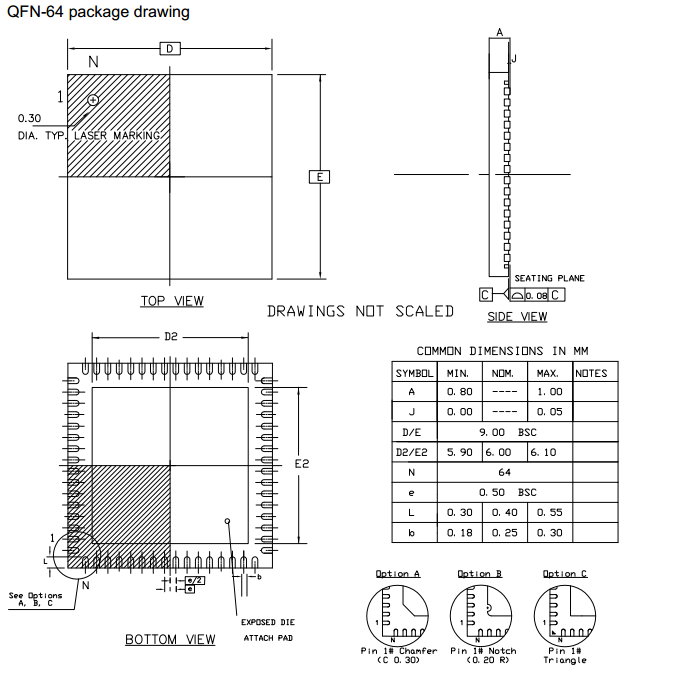
\includegraphics[height=10cm]{img/AT32UC3C2512C.png}
		\hfill \break
	\end{adjustbox}
	\pagebreak
		
	\section{Grundkonzept der Stromquelle}\hfill \break
	\begin{adjustbox}{center,caption={Grundkonzept der Stromquelle},label={fig:Grundkonzept},nofloat=figure,vspace=\bigskipamount}
		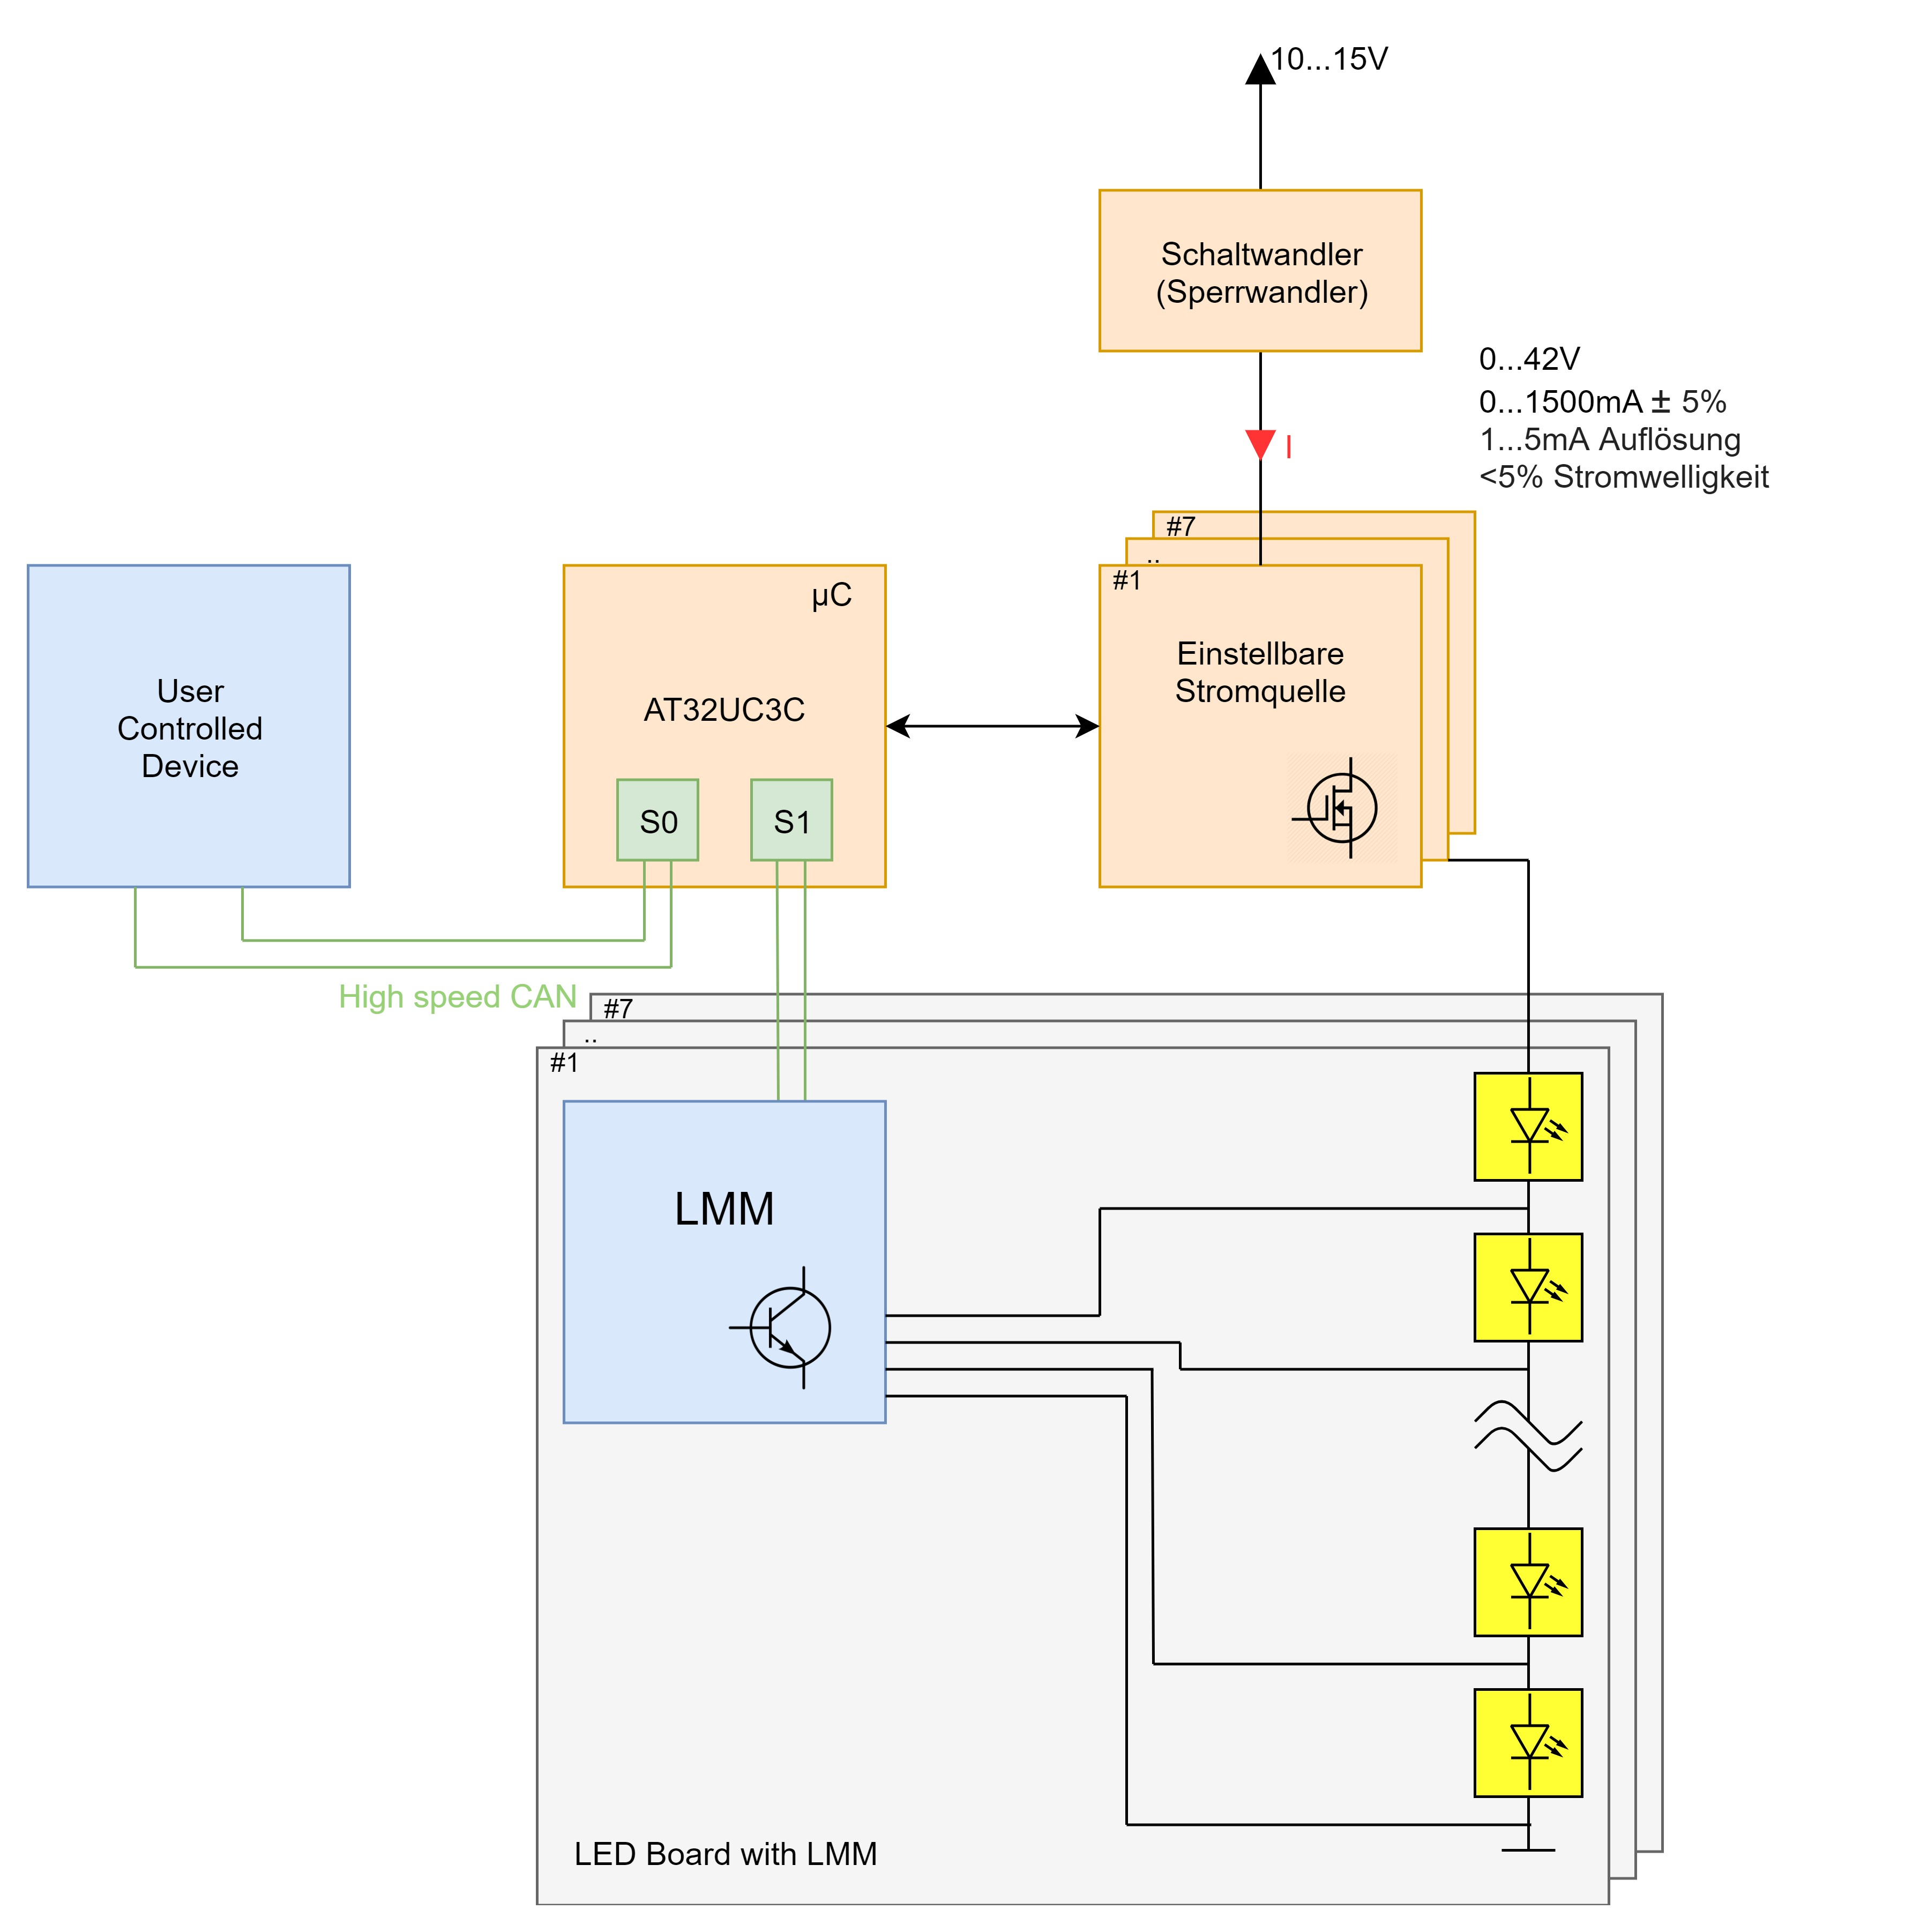
\includegraphics[height=\textwidth]{img/Diplomarbeit_Blockschaltbild.jpg}
		\hfill \break
	\end{adjustbox}
	Der Aktuelle stand des Schaltungskonzepts wurde in einem Blockschaltbild festgehalten.
	Diese Vorgehensweise war ungemein wichtig damit der Auftraggeber sich ein genaueres Bild der Arbeit machen konnte und ob das Projekt den Anforderungen gerecht entwickelt wird.
	\newpage
	
	\ifoot{Florian Hintermeier}
	\section{Programmierung}\hfill \break
	Der Verwendete Mikrocontroller ist der AT32UC3C2512C, ein 32-Bit Prozessor mit 64KB SRAM, 512KB Programmspeicher und 66MHz maximaler CPU Frequenz von Microchip.
	
	Da ein Mikrocontroller mit einer 32-Bit Architektur gewählt wurde, sind auch die Funktionen anders, als bei den in der HTL verwendeten 8-Bit Controllern. Zu beachten ist dabei, dass die Registerzugriffe vollkommen anders aussehen. Auch gibt es bei der AT32 Serie, die in dieser Diplomarbeit verwendet wurde, die Möglichkeit für jeden PIN eine von sechs verschiedenen Hardware-Funktionen zu übernehmen. Diese verschiedenen Funktionen kann man dem Datenblatt entnehmen.\footnote{http://ww1.microchip.com/downloads/en/DeviceDoc/doc32117.pdf Seite 11}
	\begin{adjustbox}{center,caption={Ausschnitt aus der Peripheral Multiplexing Tabelle},label={fig:PeripheralMultiplexRegisterTabelle.PNG},nofloat=figure,vspace=\bigskipamount}
		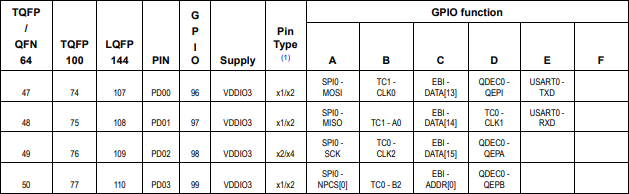
\includegraphics[width=\textwidth]{img/Peripheral_Multiplex_Register_Tabelle.PNG}
	\end{adjustbox}
	Wie oben beschrieben und auch im Bild zu sehen, kann jeder Pin bis zu sechs verschiedene Funktionen haben, in diesem Beispiel müsste man für USART RX und TX die GPIO Ports auf Mode E initialisieren.
	\lstinputlisting[language=c, caption=GPER Beispiel]{src/gpioExample.c}
	
	Die Tabelle\footnote{http://ww1.microchip.com/downloads/en/DeviceDoc/doc32117.pdf Seite 468} für das Peripheral Multiplex Register findet man auch im Datenblatt des Mikrocontrollers, dort kann man herauslesen, was bei pmr[n] eingestellt werden muss.
	\begin{adjustbox}{center,caption={Peripheral Multiplex Register Mode Tabelle},label={fig:PeripheralFunktions.PNG},nofloat=figure,vspace=\bigskipamount}
		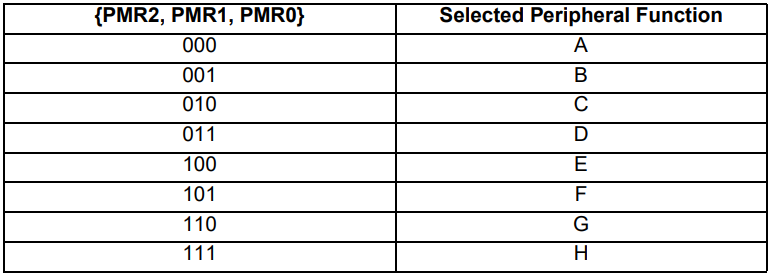
\includegraphics[height=4cm]{img/Peripheral_Funktions.PNG}
	\end{adjustbox}
	\newpage
	Um diese Mikrocontroller spezifischen Funktionen verwenden zu können, braucht man folgende Headerfiles im C-Code:
	\begin{itemize}
		\item inttypes.h
		\item avr32/io.h
	\end{itemize}

	Weitere verwendete Headerfiles:
	\begin{itemize}
		\item math.h
	\end{itemize}
	Das math.h Headerfile wird benötigt, um die Berechnungen, die für die Spannungseinstellungen nötig sind bewerkstelligen zu können. \hfill \break
	Im io.h Headerfile finden sich alle wichtigen Definitionen bezüglich der 32-Bit AVR Mikrocontroller, im Makefile des Projekts wird der Verwendeter Mikrocontroller festgelegt, so kann der C-Compiler dann alle wichtigen Definitionen, wie Ports und Register finden und dem HEX-Code für den Controller richtig zuordnen. \hfill \break
	Das Makefile und die anderen projektspezifischen Daten für ein Mikrocontroller Projekt werden von Atmel Studio nach der Konfiguration der Einstellungen erstellt. In diesen Einstellungen werden sowohl Taktfrequenz als auch Taktquelle eingestellt.
	\newpage
	
		
\ifoot{Florian Hintermeier}	
\chapter{Ergebnisse}\hfill \break
	\section{Analogteil}\hfill \break
	Da die Eingangsspannung, mit der das Gerät versorgt werden soll, zwischen 10 und 15 Volt liegt, muss man die Spannung erhöhen, was in diesem Fall mit einem SEPIC-Converter passiert. Als Basis dafür wurde der LT3757 verwendet.\hfill \break
	Die Grundbeschaltung wurde aus dem Datenblatt\footnote{https://www.analog.com/media/en/technical-documentation/data-sheets/3757Afe.pdf Seite 31} übernommen, die benötigten Bauteilwerte wurden jedoch mittels Simulationen mit LTSpice ermittelt.
	\begin{adjustbox}{center,caption={Referenzschaltung für SEPIC}, label={fig:LTSpice-Schaltung-Analogteil},nofloat=figure,vspace=\bigskipamount}
		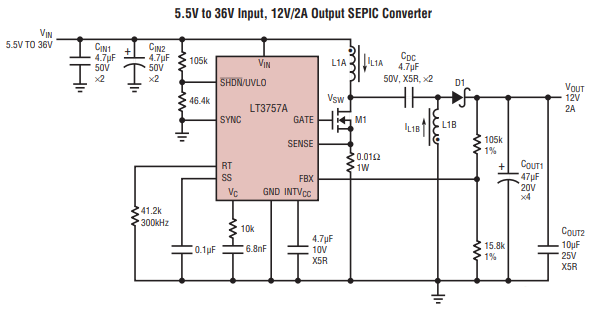
\includegraphics[height=7cm]{img/Referenzschaltung_SEPIC.PNG}
	\end{adjustbox}
	\newpage
	
		\subsection{Schaltung}\hfill \break
			\subsubsection{LTSpice}\hfill \break
			\begin{adjustbox}{angle=90, center,caption={Simulationsschaltung des Analogteils in LTSpice},label={fig:LTSpice-Schaltung-Analogteil},nofloat=figure,vspace=\bigskipamount}
				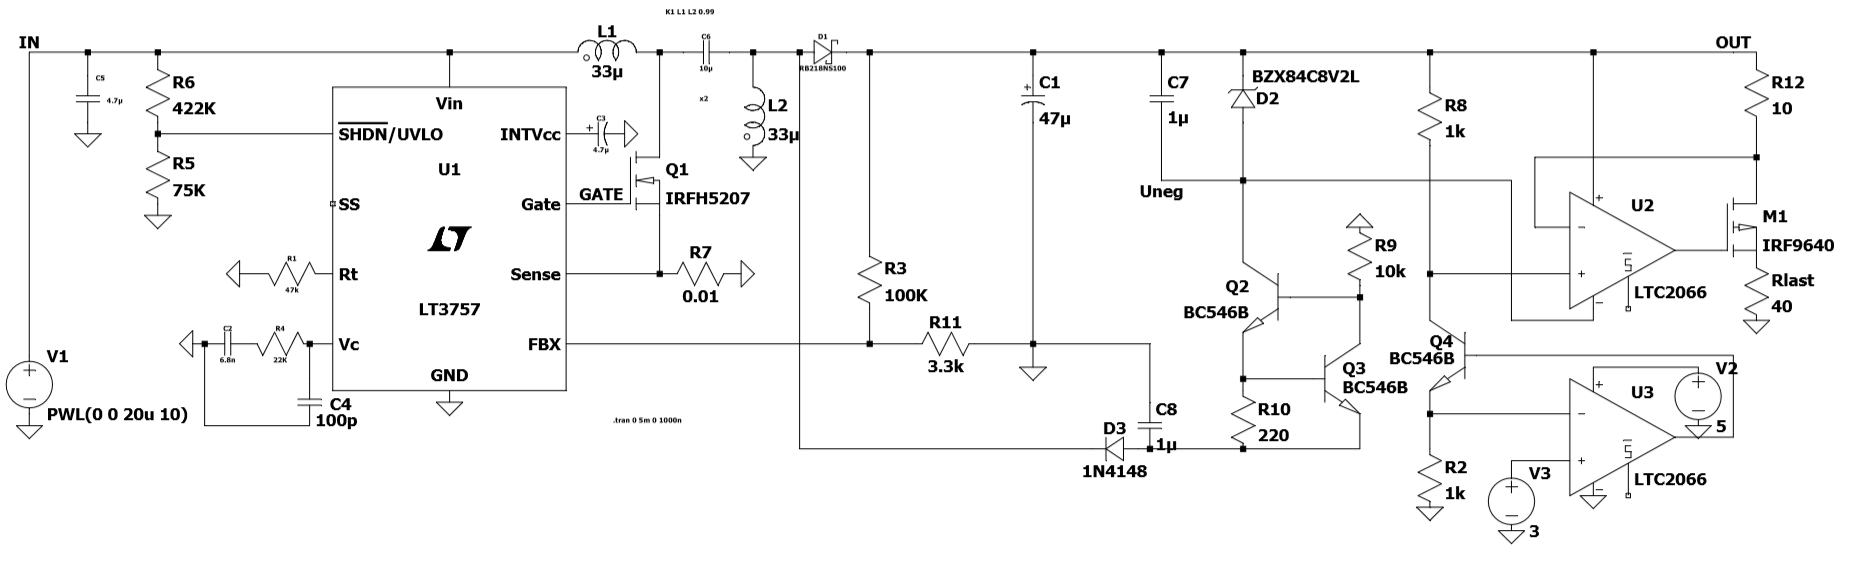
\includegraphics[width=20cm]{img/LTSpice_Schaltung_Analogteil.PNG}
			\end{adjustbox}
			\pagebreak
			\subsubsection{Altium}\hfill \break
			Die Schaltung in Altium wurde für eine bessere Übersicht in mehrere Teile aufgeteilt. Um trotzdem die Verbindung zwischen den einzelnen Leitungen herzustellen wurden sogenannte Ports verwendet. Das sind Verbindungen mit gleichnamigen Kästchen. Wie man auf den einzelnen Schaltungselementen auch erkennen kann, wurde für den Analogteil der Zahlenbereich von 200 bis 299 für die Benennung der Bauteile verwendet. Dies dient zum besseren Erkennen der Schaltungszugehörigkeit beim Entwickeln des PCBs.
			\paragraph{SEPIC}\hfill \break
			\begin{adjustbox}{center,caption={Grundbeschaltung des LT3757},label={fig:LT3757-Grundbeschaltung},nofloat=figure,vspace=\bigskipamount}
				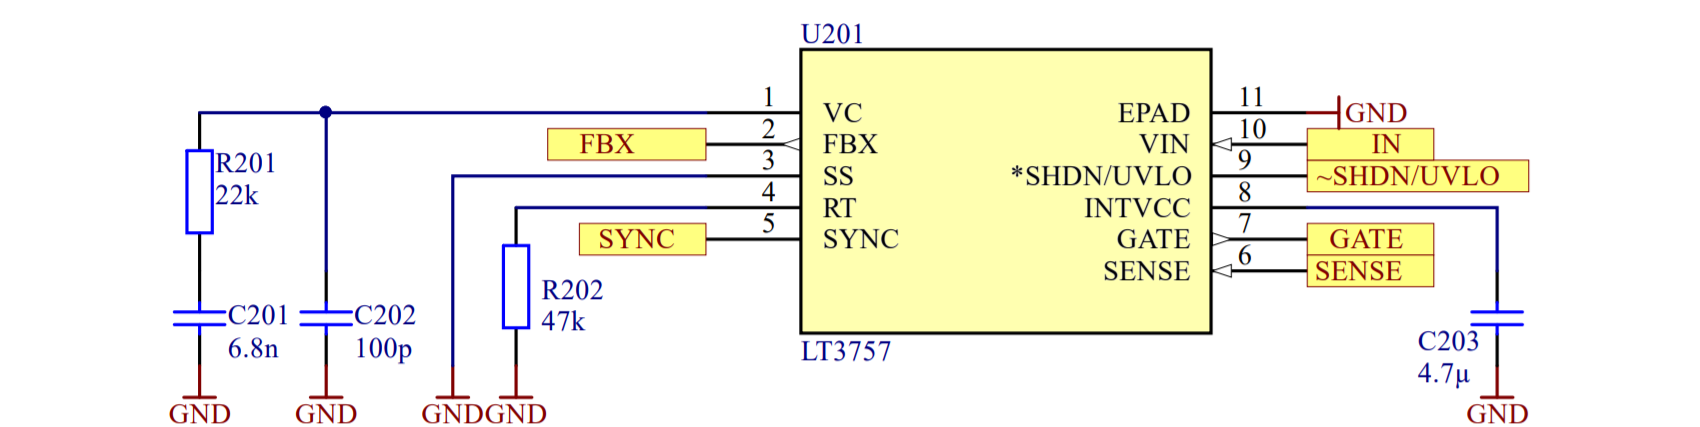
\includegraphics[width=\textwidth]{img/SEPIC_Altium.PNG}
			\end{adjustbox}
			Oben abgebildet ist die Grundbeschaltung des SEPIC-Chip LT3757. Das RC-Netzwerk bei dem VC-Pin hält die Spannung für die Erzeugung der internen Spannung stabil. Am RT-Pin wird mittels des Widerstandes eine Schaltfrequenz eingestellt. Der Pin INTVCC ist da um die Spannungen für die interne Versorgung und das Gate stabil zu halten.
			\paragraph{Undervoltage Shutdown für SEPIC}\hfill \break
			\begin{adjustbox}{center,caption={Undervoltage Shutdown Schaltung für LT3757},label={fig:uvlo},nofloat=figure,vspace=\bigskipamount}
				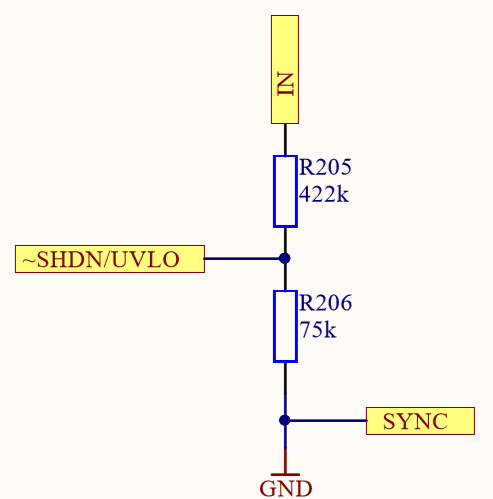
\includegraphics[width=\textwidth]{img/Undervolteage_Shutdown_SEPIC.PNG}
			\end{adjustbox}
			Dieser Teil der Schaltung ist dafür zuständig, dass die Spannung am Eingang überprüft wird, ist die Spannung zu klein, wird der SEPIC-Chip deaktiviert um keine Schäden verursachen zu können.
			\pagebreak
			\paragraph{Feedback Schaltung für SEPIC}\hfill \break
			\begin{adjustbox}{center,caption={Feedback Schaltung für SEPIC},label={fig:feedback},nofloat=figure,vspace=\bigskipamount}
				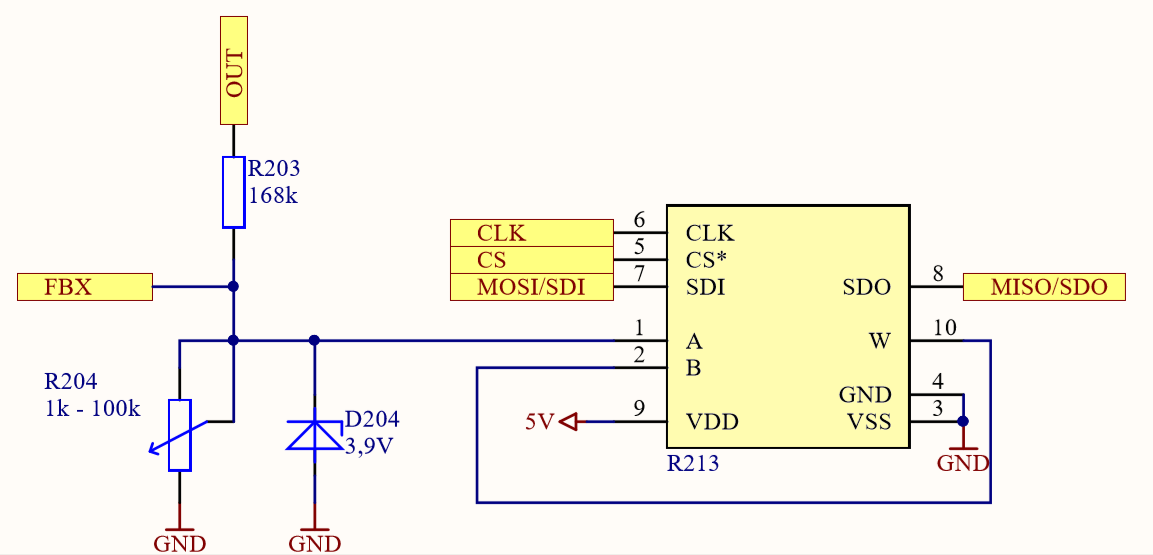
\includegraphics[width=\textwidth]{img/Feedback_SEPIC.PNG}
			\end{adjustbox}
			Dieser Teil ist zuständig für das Feedback der Spannung, die die Schaltfrequenz des FETs einstellt, über den auch die Ausgangsspannung eingestellt wird. Eingestellt wird die Schaltfrequenz mit dem Spannungsteiler von R203 und R204/R213, welcher der beiden verwendet wird, hängt von der Jumper Einstellung ab, es soll immer so sein, dass die Spannung am FBX-PIN 1,6 Volt beträgt.
			
			Die Z-Diode wird deshalb benötigt, weil die Spannung bei Änderung des Widerstandes höher werden kann, es wird dann vom LT3757 geregelt, dass innerhalb kürzester Zeit wieder die gewollten 1,6V anliegen. Jedoch ist es für das digitale Potentiometer schädlich, wenn eine Spannung höher als die Versorgungsspannung anliegt. Deshalb wurde die Z-Diode verbaut, um die maximale Spannung, die anliegt auf 3,9V zu begrenzen.
			\paragraph{Regelung für SEPIC}\hfill \break
			\begin{adjustbox}{center,caption={Regelungsschaltung für LT3757},label={fig:regelung},nofloat=figure,vspace=\bigskipamount}
				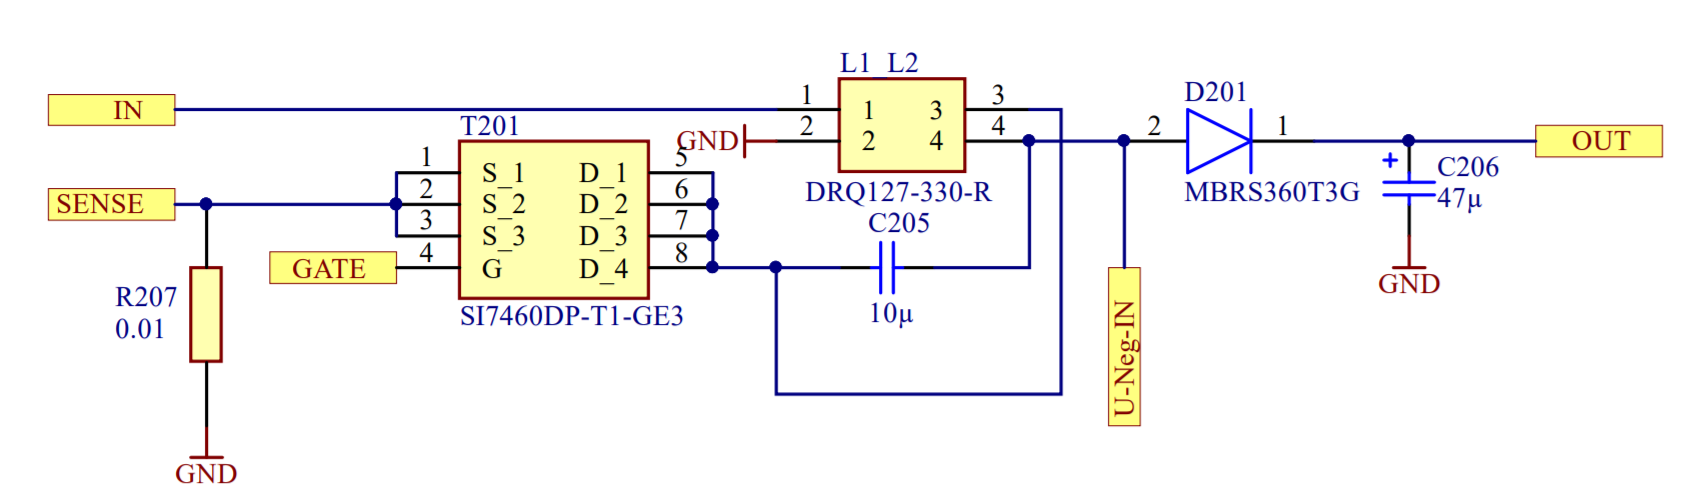
\includegraphics[width=\textwidth]{img/Regelung_SEPIC.PNG}
			\end{adjustbox}
			Der SENSE-PIN misst den Strom am FET, wenn der zu groß ist, wird die Regelung ausgeschaltet. Die Spulen L1 und L2 sind gegengleich gekoppelt mit einem Verhältnis von 1 zu 1. Am Ausgang (OUT) liegt dann die mit den Widerständen von der Feedback Schaltung eingestellte Spannung.
			\pagebreak
			\paragraph{Negative Spannung}\hfill \break
			\begin{adjustbox}{center,caption={Schaltung für Versorgung von OPV der Stromquelle},label={fig:neg-spg},nofloat=figure,vspace=\bigskipamount}
				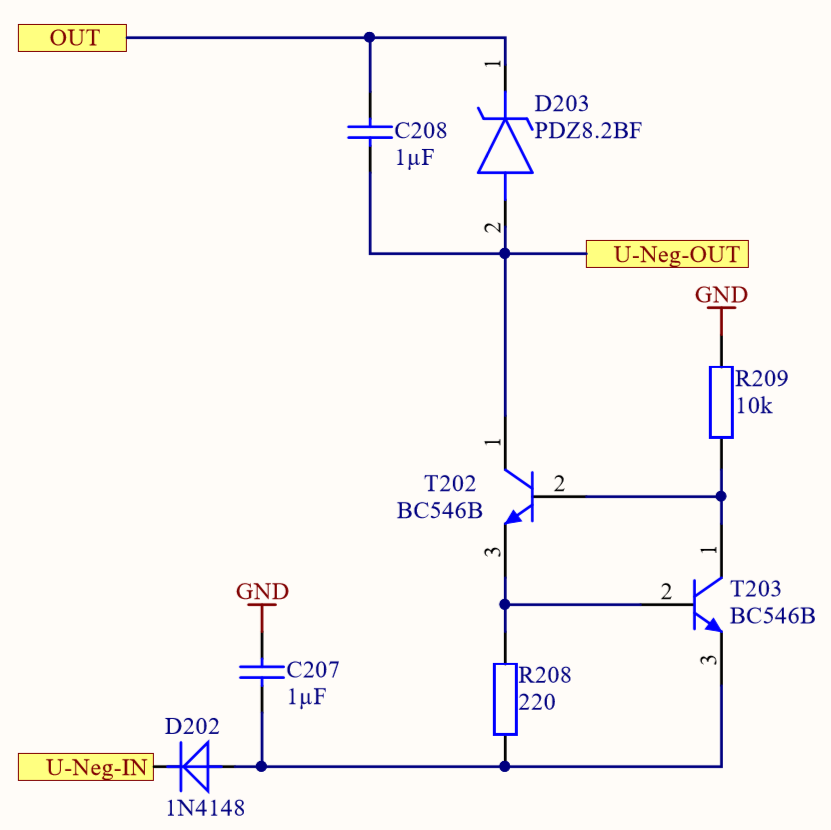
\includegraphics[width=\textwidth]{img/Negative_Spannung.PNG}
			\end{adjustbox}
			Diese Schaltung dient dazu, eine Spannung zu erzeugen, die immer 8,2V unter der Spannung von (OUT) liegt. Die niedrigere Spannung liegt an dem Punkt U-Neg-OUT. In einer Simulation in Abbildung \ref{fig:LTSpice-Simulation-1} kann man den Spannungsunterschied zwischen V(out) und V(uneg) sehen.
			\newpage
			\paragraph{Stromquelle}\hfill \break
			\begin{adjustbox}{center,caption={Schaltung für die Einstellbare Stromquelle},label={fig:stromquelle},nofloat=figure,vspace=\bigskipamount}
				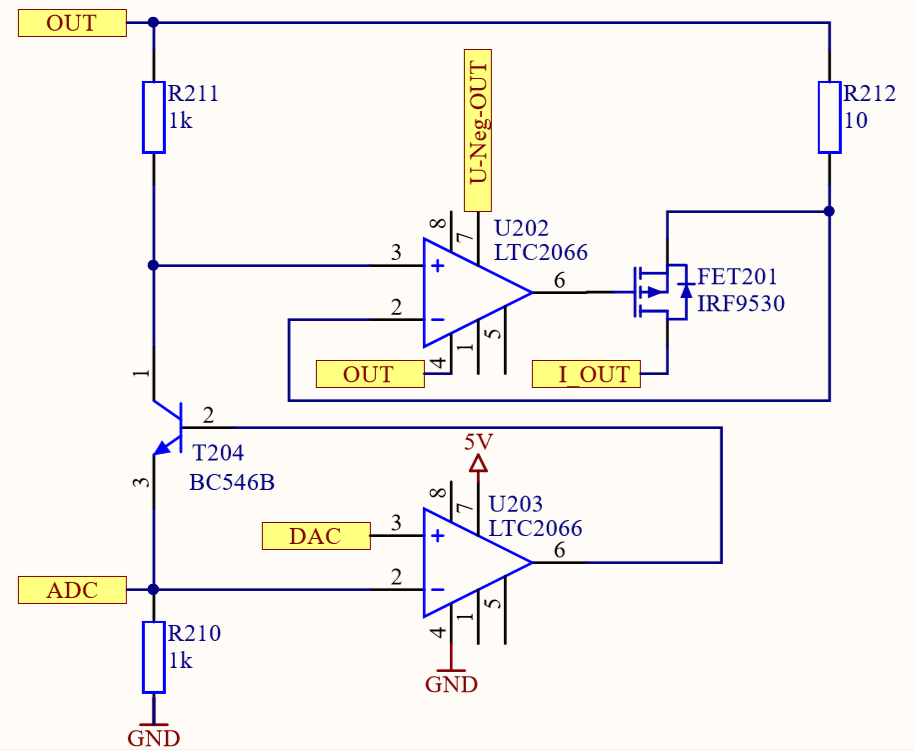
\includegraphics[width=\textwidth]{img/Stromquelle_SEPIC.PNG}
			\end{adjustbox}
			Bei dieser Schaltung wird ein Stromspiegel verwendet um den Strom mit dem ADC des Mikrocontrollers messen zu können. Weiters wird der maximale Strom mit der Spannung am Plus Eingang des OPV (U203) mit dem DAC des Mikrocontrollers eingestellt.\newpage
			
		\subsection{Simulation}\hfill \break
			Mithilfe von LTSpice war es möglich, die Schaltung zu analysieren und ihre ungefähren Eigenschaften herauszufinden. Es wurden Spannungsverläufe und auch Zeiten damit ermittelt, die einen wichtigen Beitrag zur Vorbereitung auf die Programmierung geleistet haben.
			\begin{adjustbox}{center,caption={Simulation der Schaltung Mittels LTSpice},label={fig:LTSpice-Simulation-1},nofloat=figure,vspace=\bigskipamount}
				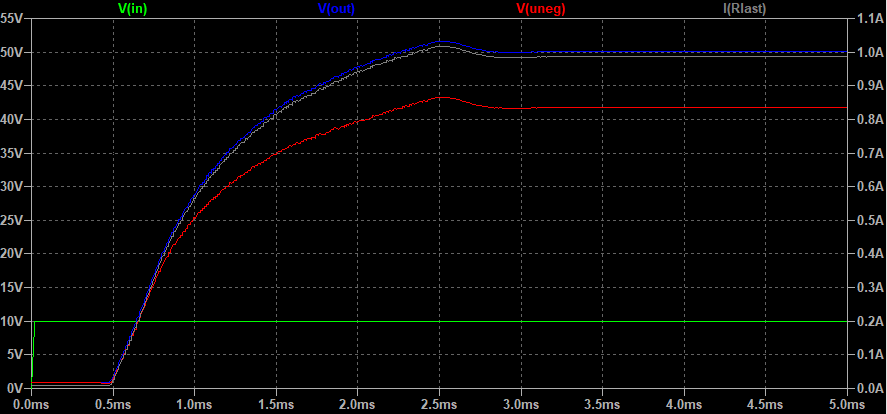
\includegraphics[width=\textwidth]{img/LTSpice_Simulation_1.PNG}
			\end{adjustbox}
			Wie in Abbildung \ref{fig:LTSpice-Simulation-1} zu sehen, ist in der Simulation die Eingangsspannung(in) auf 10 Volt eingestellt, der SEPIC-Converter braucht hier ca. 2,75ms um die Ausgangsspannung(out) auf konstante 50 Volt einzustellen. Bei der simulierten Belastung von 40 Ohm(Rlast) wird ca. 1 Ampere aus der Schaltung gezogen. Das entspricht auch den Leistungsanforderungen der Firma, welche die maximale benötigte Ausgangsleistung mit 40 Watt angegeben hat.
			
			\begin{align*} 
			P_{out} = U_{out} \cdot I_{Rlast} = 50V \cdot 1A = 50W
			\end{align*} 
			
			Laut Simulation hat diese Schaltung eine Ausgangsleistung von 50W, was sogar mehr ist als angegeben. 
			\begin{adjustbox}{center,caption={Stabile Gate Spannung des MOSFETs},label={fig:LTSpice-Simulation-2},nofloat=figure,vspace=\bigskipamount}
				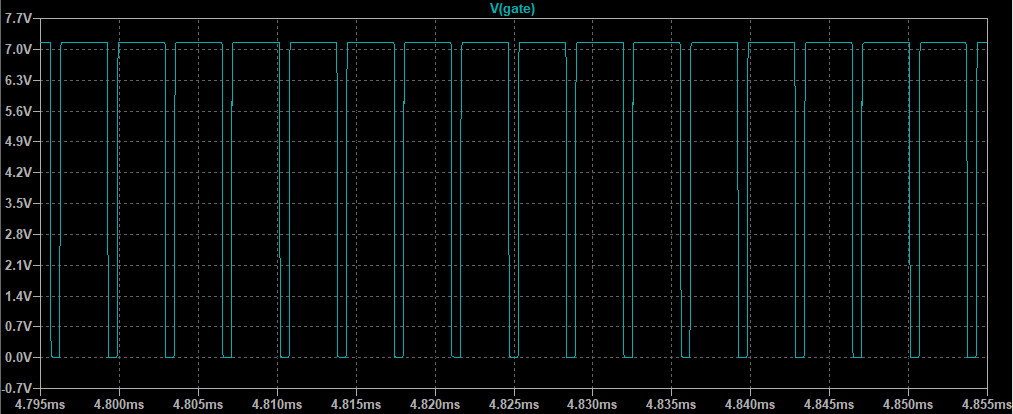
\includegraphics[width=\textwidth]{img/LTSpice_Simulation_2.PNG}
			\end{adjustbox}
			
			Die Frequenz am GATE ist nach ca 2,75ms stabil, genauso wie V(out) in Abbildung \ref{fig:LTSpice-Simulation-1} zu sehen, ist. 
			
			\subsubsection{Spannungseinstellung}\hfill \break
			Um herauszufinden wie sich die Spannung bei Widerstandsänderung verändert, wurde dies auch mithilfe von LTSpice herausgefunden.
			
			Grundsätzlich ist es so:
			\begin{itemize}
				\item Hoher Widerstand -> Niedrige Spannung
				\item Niedriger Widerstand -> Hohe Spannung
			\end{itemize}
			
			Es ist schon bekannt, dass 50V die maximale Spannung ist, die noch stabil eingestellt werden kann. Diese Simulation hat ergeben, dass die niedrigste einstellbare Spannung 3,21V beträgt.
			
			Einige Werte dazwischen sind in diesem Diagramm abzulesen:
			\begin{adjustbox}{center,caption={Spannungsverlauf bei Widerstandsänderung},label={fig:spgVLbWdst},nofloat=figure,vspace=\bigskipamount}
				\includegraphics[width=\textwidth]{img/simulationSPG.PNG}
			\end{adjustbox}
		
			In dem Diagramm kann man sehen, dass die Zeit bis sich die Ausgangsspannung stabilisiert und immer kürzer wird, je näher man der Eingangsspannung kommt, diese war in diesem Fall 10V. Das liegt daran, dass die Schaltung weniger herunter oder hinauf wandeln muss, wenn die Ausgangsspannung der Eingangsspannung näher ist.
		
			\subsubsection{Ergebnisse der Simulationen}\hfill \break
			{\large \textbf{Maximale Spannung:} 51,2V} \hfill \break
			{\large \textbf{Minimale Spannung:} 3,2V}\hfill \break
			{\large \textbf{Stabiler Spannungszustand:} nach durchschnittlich 1,74ms} \hfill \break
			
			\subsubsection{Berechnungen}\hfill \break
			\label{sec:berechnungen}
			Aufgrund der Simulation der Spannungseinstellungen weiß man, wie die Spannungskurve aussieht. Auf Grundlage dieser wurde eine Hyperbelfunktion aufgestellt, welche die Berechnungen für die einzustellenden Widerstandswerte für das Mikrocontroller-Programm ermöglicht. \hfill \break
			Erstellt wurde diese Funktion mithilfe GeoGebra, welches sich perfekt dafür eignet Kurven anzeigen zu lassen. Zuerst wurden die Werte aus der Simulation in Punkten dargestellt um die Funktionskurve langsam an die Simulationskurve anpassen zu können. \hfill \break
			Die Richtigkeit der Formel wurde überprüft, indem die Werte für den Widerstand aus der Simulation für die Variable R eingesetzt wurden und das gleiche Ergebnis herauskam. \hfill \break \hfill \break
			\textbf{Die Funktion:} 
			\begin{align*} 
			U_{out}(R) = 200 \cdot R^{-1,1} + 2
			\end{align*}
			Die Kurve der Funktion passt zu den benötigten Spannungswerten ab einem Widerstandswert von 4Ω. Alle Spannungswerte zwischen Widerstandswerten von 4Ω und 100Ω passen zu denen aus der Simulation.
			\begin{adjustbox}{center,caption={Berechneter Spannungsverlauf bei Widerstandsänderung},label={fig:berechnungSPG},nofloat=figure,vspace=\bigskipamount}
				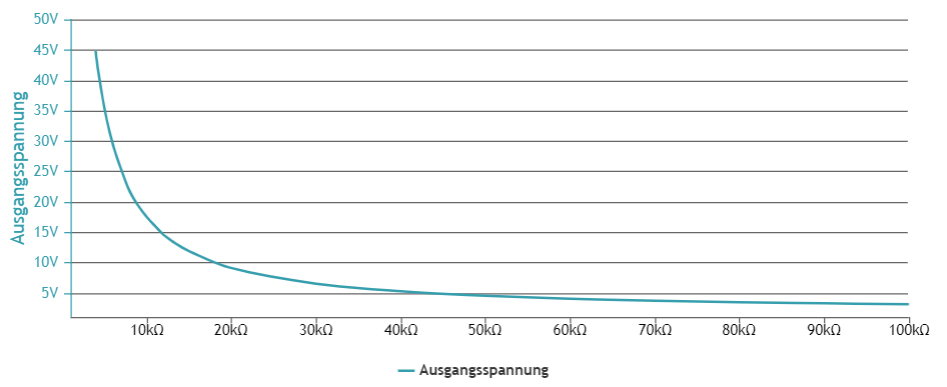
\includegraphics[width=\textwidth]{img/berechnungSPG.PNG}
			\end{adjustbox}
			Im späteren Verlauf wird die einzustellende Spannung bekannt gemacht, da man vom UCD die einzuschaltenden LEDs übertragen bekommt. Das heißt man muss in diesem Fall nicht nach der Ausgangsspannung berechnen, da diese bekannt ist, sondern nach dem Widerstandswert. \hfill \break \hfill \break
			\textbf{Formel zur Berechnung des Widerstandswertes:}
			\begin{align*} 
			R=\frac{ U - 2 }{ 200 }^{ -\frac{ 1 }{ 1,1 } }
			\end{align*}
			\textbf{Formel zur Berechnung des Widerstandswertes in C Code:}
			\lstinputlisting[language=c, caption=C-Code für Widerstandsberechnung]{src/widerstandBerechnung.c}
			 
			\subsubsection{Simulation eines Anwendungsfalls}\hfill \break
			Von der Firma ZKW kommen verschiedene Anwendungsfälle. Um zu Testen, ob die Schaltung so funktioniert, wie sie es brauchen, wird einer der Fälle simuliert, statt dem LED-Strang kommt in der Simulation ein Widerstand zum Einsatz, an dem Gleich viel Spannung abfällt.
			\begin{adjustbox}{center,caption={Anwendungsfall von ZKW},label={fig:anwendungsfall},nofloat=figure,vspace=\bigskipamount}
				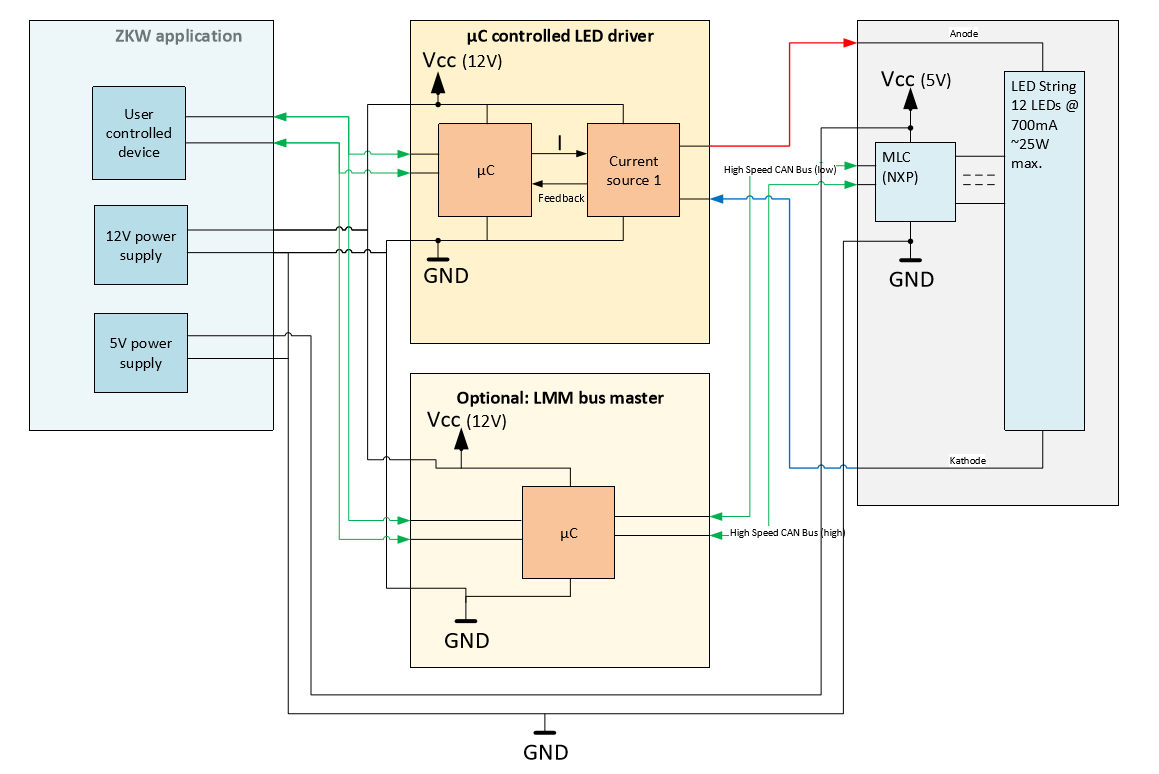
\includegraphics[width=\textwidth]{img/SimulierterAnwendungsfall.PNG}
			\end{adjustbox}
			In diesem Fall brauchen die LEDs eine Spannung von 35V. Wie aus dem Diagramm herauszulesen, wird der Widerstand in der Simulation geändert auf 4.4kΩ. Das ist zwar eine Spannung von 37V, da die Schaltung für die Strommessung und Einstellung selbst ein paar Volt braucht, 2V um genau zu sein. Somit sind die 35V für die LEDs zu haben. 
			\newpage
			
	\ifoot{Dominik Gansch}	
	\section{Digitalteil}
	Als perfekte Wahl stellte sich der AT32UC3C2512C von Microchip heraus. Dieser erfüllt alle Anforderungen und ist noch dazu Preiswert. Die Grundbeschaltung wurde aus den Empfehlungen des Datenblattes erstellt und anwendungsspezifisch erweitert.
		\subsection{Schaltung}
		\begin{adjustbox}{center,caption={Mikrocontroller Grundbeschaltung},label={fig:uC Grundbeschaltung},nofloat=figure,vspace=\bigskipamount}
			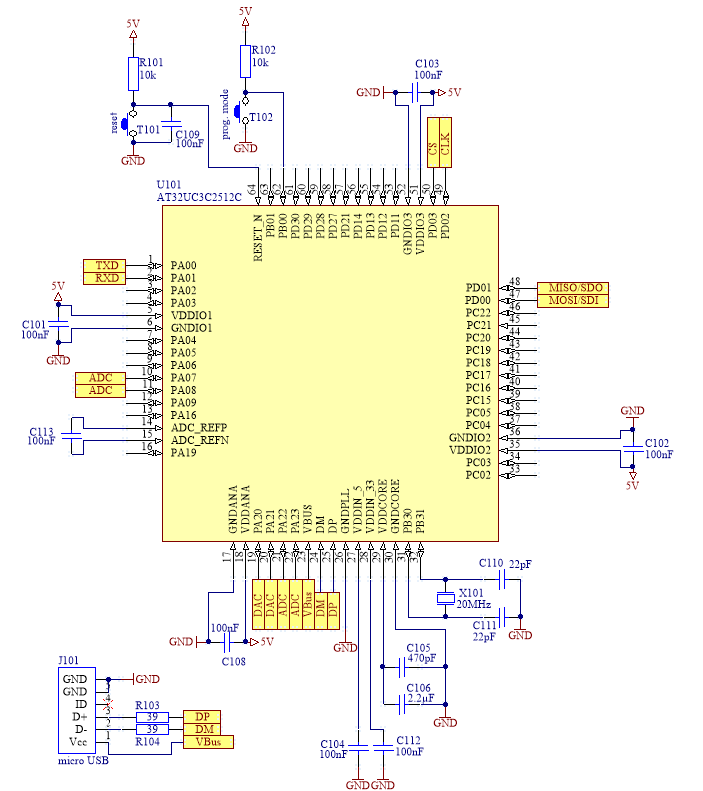
\includegraphics[width=\textwidth]{img/Grundbeschaltung_uC.PNG}
		\end{adjustbox}
	Fast alle passiven Bauelemente welche in der Abbildung \ref{fig:uC Grundbeschaltung} zu sehen sind werden für die Grundfunktionen benötigt. Die Kondensatoren (C110 \& C111) beim 16MHz Quarz (X101) werden für den internen Oszillator benötigt. Für die Stabilität des internen LDO wurden die Kondensatoren mit 100nF \& 470pF dimensioniert.
	Alle anderen Kondensatoren sind Stützkondensatoren. Die Taster (T101 \& T101) werden für die Programmierung oder auch für den Reset des Mikrocontrollers benötigt. Die Programmierung erfolgt über USB und als physikalische Schnittstelle wurde eine Mikro-USB Buchse gewählt. Für die Spannungsteuerung des Analogteils wurde ein Digitales-Poti verwendet welches über die SPI-Schnittstelle (MISO/SDI und MOSI/SDO) angesteuert wird, des weiteren werden der interne DAC und ADC auch für die Stromregelung verwendet.
		\begin{adjustbox}{center,caption={CAN-Transceiver},label={fig:CAN-Transceiver},nofloat=figure,vspace=\bigskipamount}
		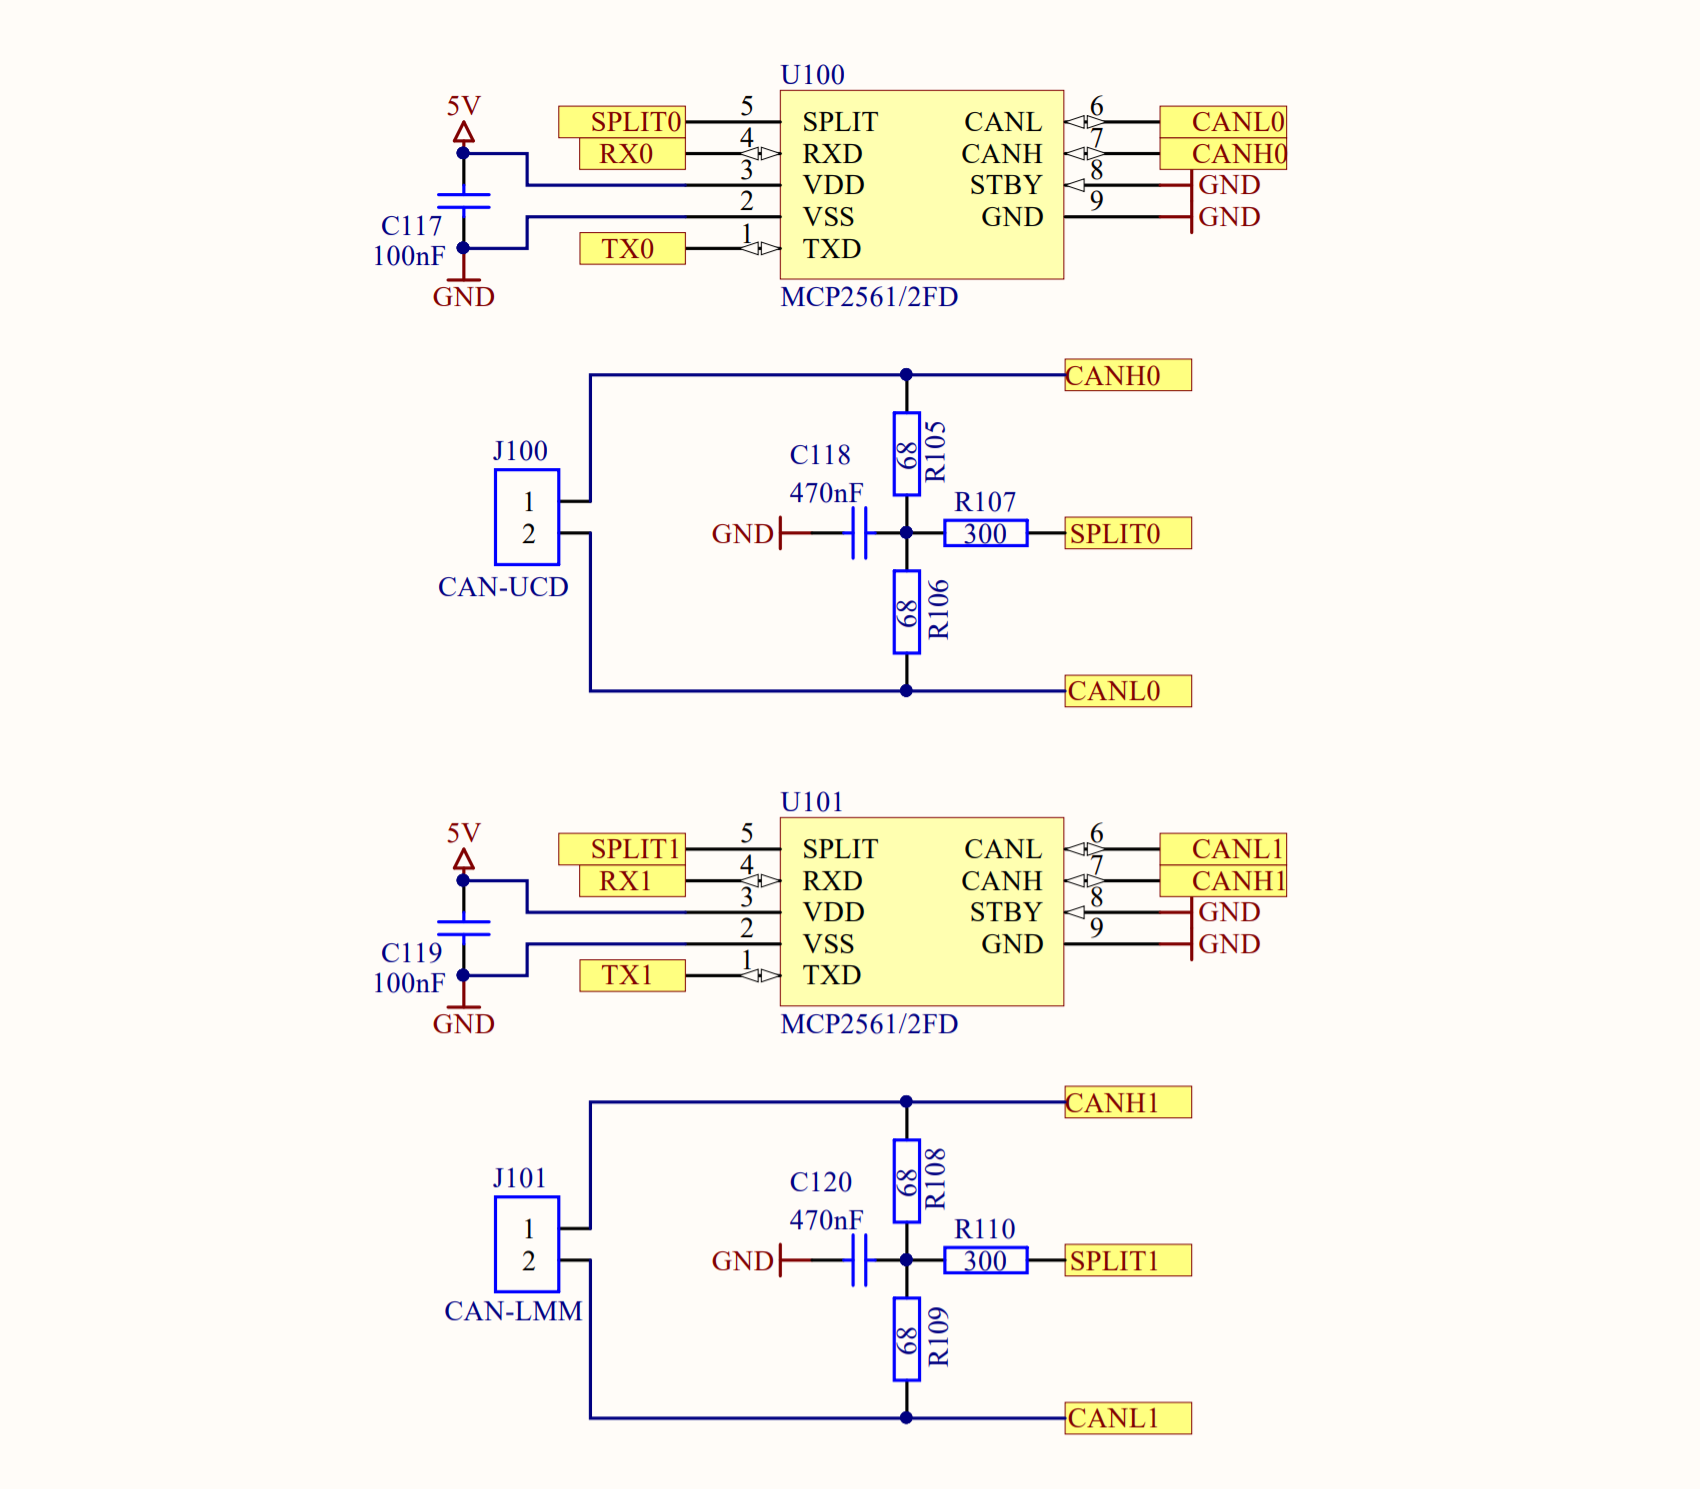
\includegraphics[width=\textwidth]{img/CAN_Tranceiver.PNG}
		\end{adjustbox}
	Die CAN-Transceiver setzten die Logikpegel, der Daten (von ursprünglichen 5V), in CAN-Bus kompatible Pegel um. In Abbildung \ref{fig:CAN-Bus-Pegel} ist eine Veranschaulichung der CAN-Bus Pegel ersichtlich.
	
	\begin{adjustbox}{center,caption={CAN-Bus Pegelumsetzung},label={fig:CAN-Bus-Pegel},nofloat=figure,vspace=\bigskipamount}
		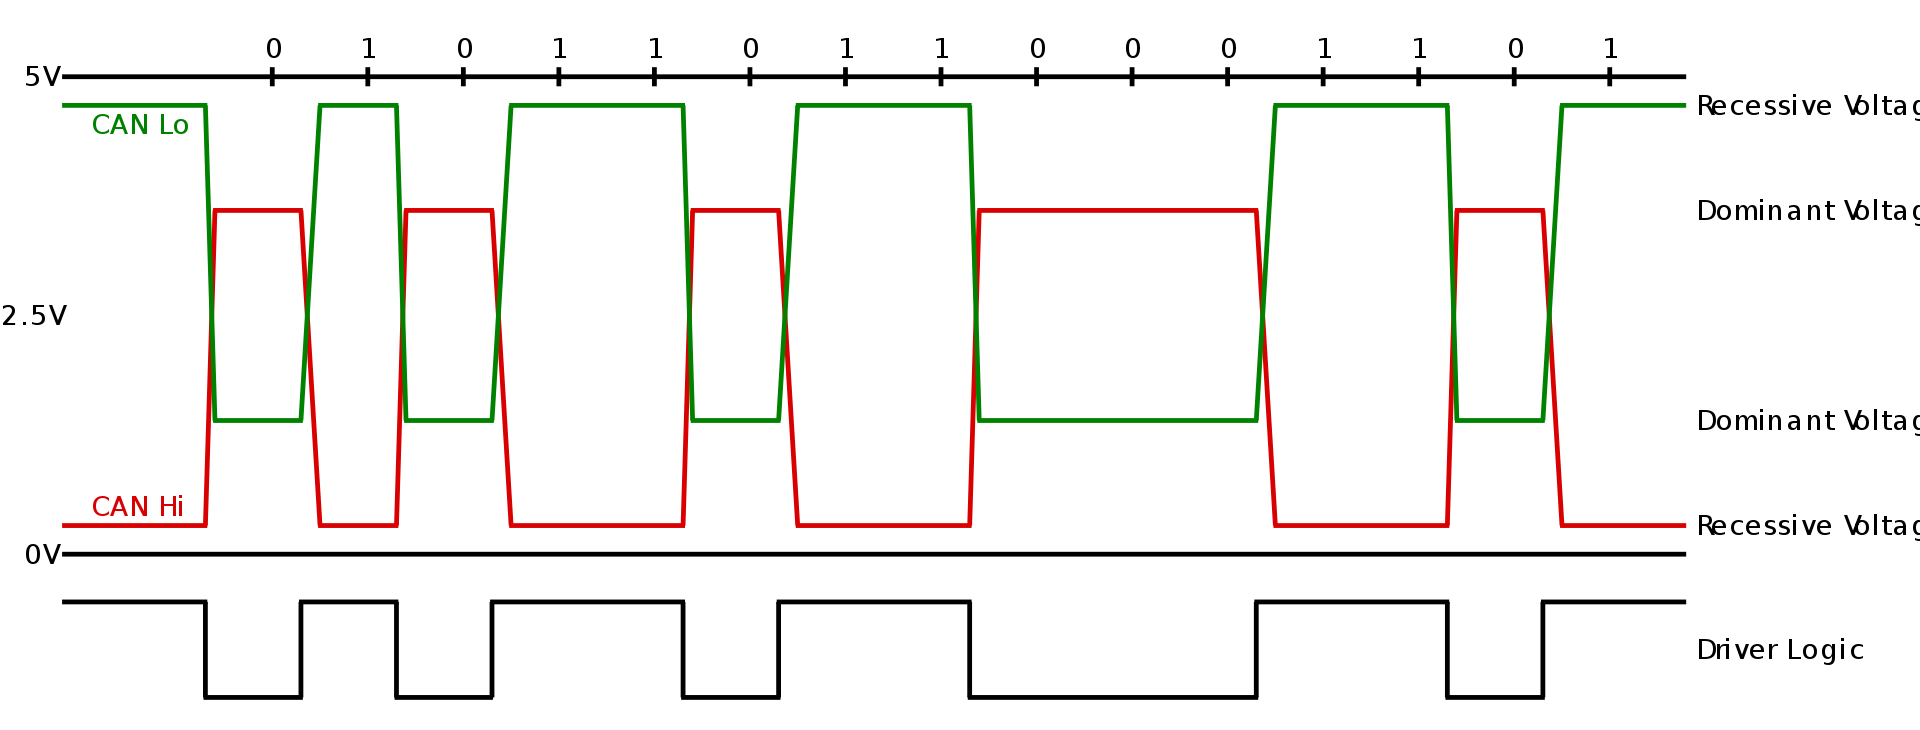
\includegraphics[width=\textwidth]{img/CAN-Pegelumsetzung.PNG}\footnote{https://upload.wikimedia.org/wikipedia/commons/thumb/4/44/ISO11898-3\_Waveform.svg/1920px-ISO11898-3\_Waveform.svg.png}
	\end{adjustbox}
	\hfill \break

	\begin{adjustbox}{center,caption={VoltageRegulator 7805 },label={fig:VoltageRegulator.PNG},nofloat=figure,vspace=\bigskipamount}
		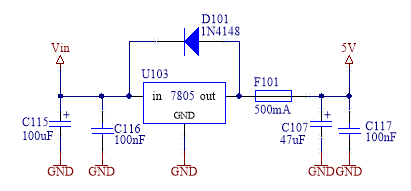
\includegraphics[width=\textwidth]{img/VoltageRegulator.PNG}
	\end{adjustbox}
 	Die Versorgungsspannung von 10...15V wurde mithilfe eines Low Drop Regulators (LDO) auf die Betriebsspannung (5V) der digitalen Bauteile geregelt. Die Diode (D101) und die selbstrückstellende Sicherung (F101) wurden als Schutzmaßnahmen integriert.
	\newpage
	
	\section{Hardware}\hfill \break
	Die Firma ZKW möchte für zahlreiche in Entwicklung und bereits in Produktion befindliche LED Einheiten einen universell einsetzbaren LED Treiber mit linear einstellbarem Strom. Es gibt bereits viele Stromquellen, welche auch sehr effizient sind, jedoch nur jeweils für den dafür entwickelten Scheinwerfer. 
	Das Ziel liegt darin, eine geeignete Hardware zu entwickeln, welche von der Baugröße gut handhabbar ist und über ein UCD gesteuert werden kann.
	Die Spannung kann anwendungsspezifisch hoch- und herunter-gewandelt werden. Wobei diese von der Anzahl der in serie geschalteten LEDs abhängt z.B.  wenn 9 LEDs in Serie geschaltet sind, entspricht das bei einer Nennspannung von 3,2V (pro LED) 28,8V.
	Der Strom kann auch anwendungsspezifisch eingestellt werden, das heißt die Schaltung liefert nur bis zu einen begrenzten Wert Strom z.B. 1,25A.
		\subsection{PCB}\hfill \break
		Folgende Dinge wurden beim Design beachtet:
		\hfill \break 
		\begin{center}
			\begin{minipage}{0.5\textwidth}
				\begin{itemize}
					\item größentechnisch praktikables Design 
					\item Benutzerfreundlichkeit
					\item Platz für möglicherweise benötigte Entstörbauteile (Filter)
					\item Kühlflächenplatz reserviert
					\item Designrules von PCB-Hersteller
					\item Designrules von Bauteilhersteller
				\end{itemize}
			\end{minipage}
		\end{center}
		\hfill \break
		Die größe des PCBs beträgt 85 mm x 70mm, so finden mehrere Module auf einer Eurokarte Platz. Da auf Benutzerfreundlichkeit geachtet wurde ist jeder Ein-, Ausgangsstecker und jedes Potentiometer nach deren Funktion beschriftet. Auch wurden zusätzliche Lötpads (R207) an Teilen der Schaltung hinzugefügt wo möglicherweise Störungen auftreten können. So kann man die Schaltung, Hardwareseitig, auch nachträglich noch durch Filter optimieren. Der Kühlflächenplatz wurde so gelöst das sich diese auf der kompletten Rückseite des PCBs befindet (Kühlung des Mosfets FET201). Das heißt die komplette Rückseite ist mit einen Kühlkörper belegt. Dies ist möglich da das PCB so designt wurde das auf dieser Seite keine Bauteile montiert werden. Damit es zu möglichst keinen Komplikationen kommt wurde auf Designrules seitens des PCB-Herstellers und der Bauteilhersteller geachtet. Auch wurde beachtet das auf Leitungen mit hoher Strombelastung möglichst kurz und breit gehalten werden. All das kann man in \ref{fig:Ausschnitt des PCB-Designs} feststellen.\hfill \break 
		\begin{adjustbox}{center,caption={Ausschitt des Designs },label={fig:Ausschnitt des PCB-Designs},nofloat=figure,vspace=\bigskipamount}
			%%	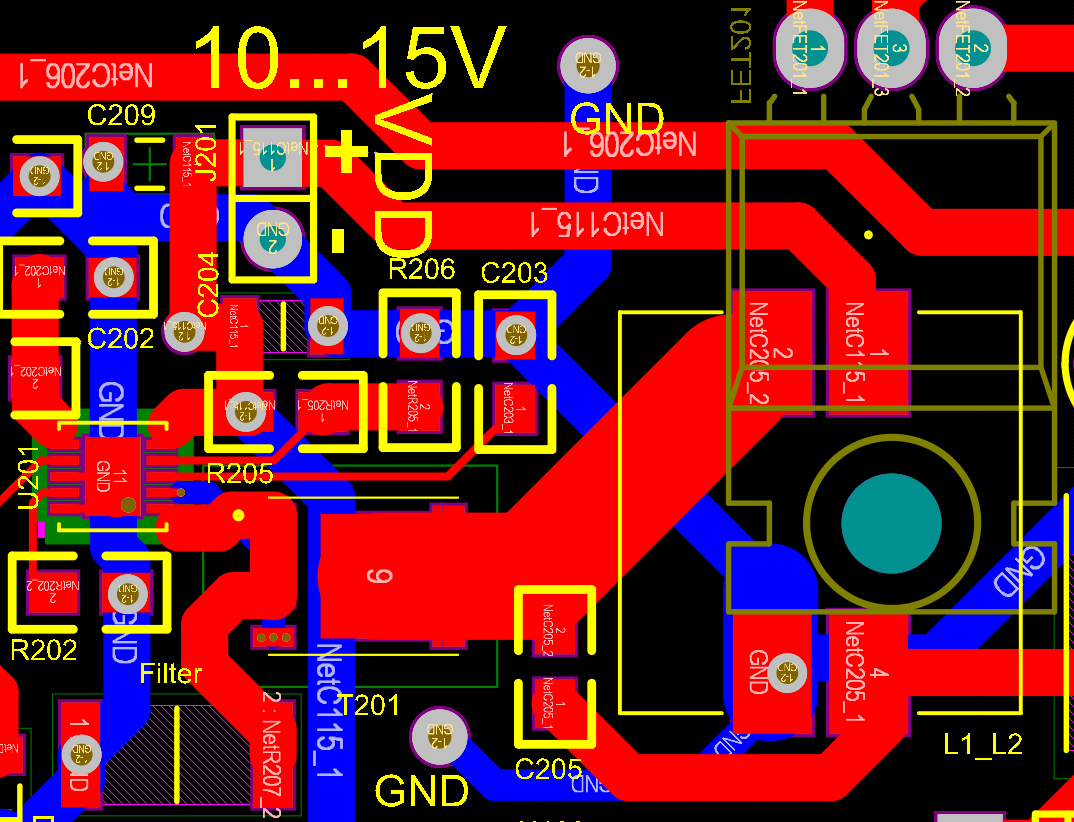
\includegraphics[width=\textwidth]{img/PCB-Design.PNG}
		\end{adjustbox}
	\newpage
	\ifoot{Florian Hintermeier}	
	\section{Software}\hfill \break
		\subsection{Programmablauf}\hfill \break
		Um die Programmierung bestmöglich umsetzen zu können, ist es sinnvoll einen Programmablaufplan zu erstellen, mithilfe davon ist es einfacher Abläufe des Programms zu Planen und diese auch nachzuvollziehen und zu verstehen.
		\begin{adjustbox}{center,caption={Programmablaufplan},label={fig:PAP.png},nofloat=figure,vspace=\bigskipamount}
			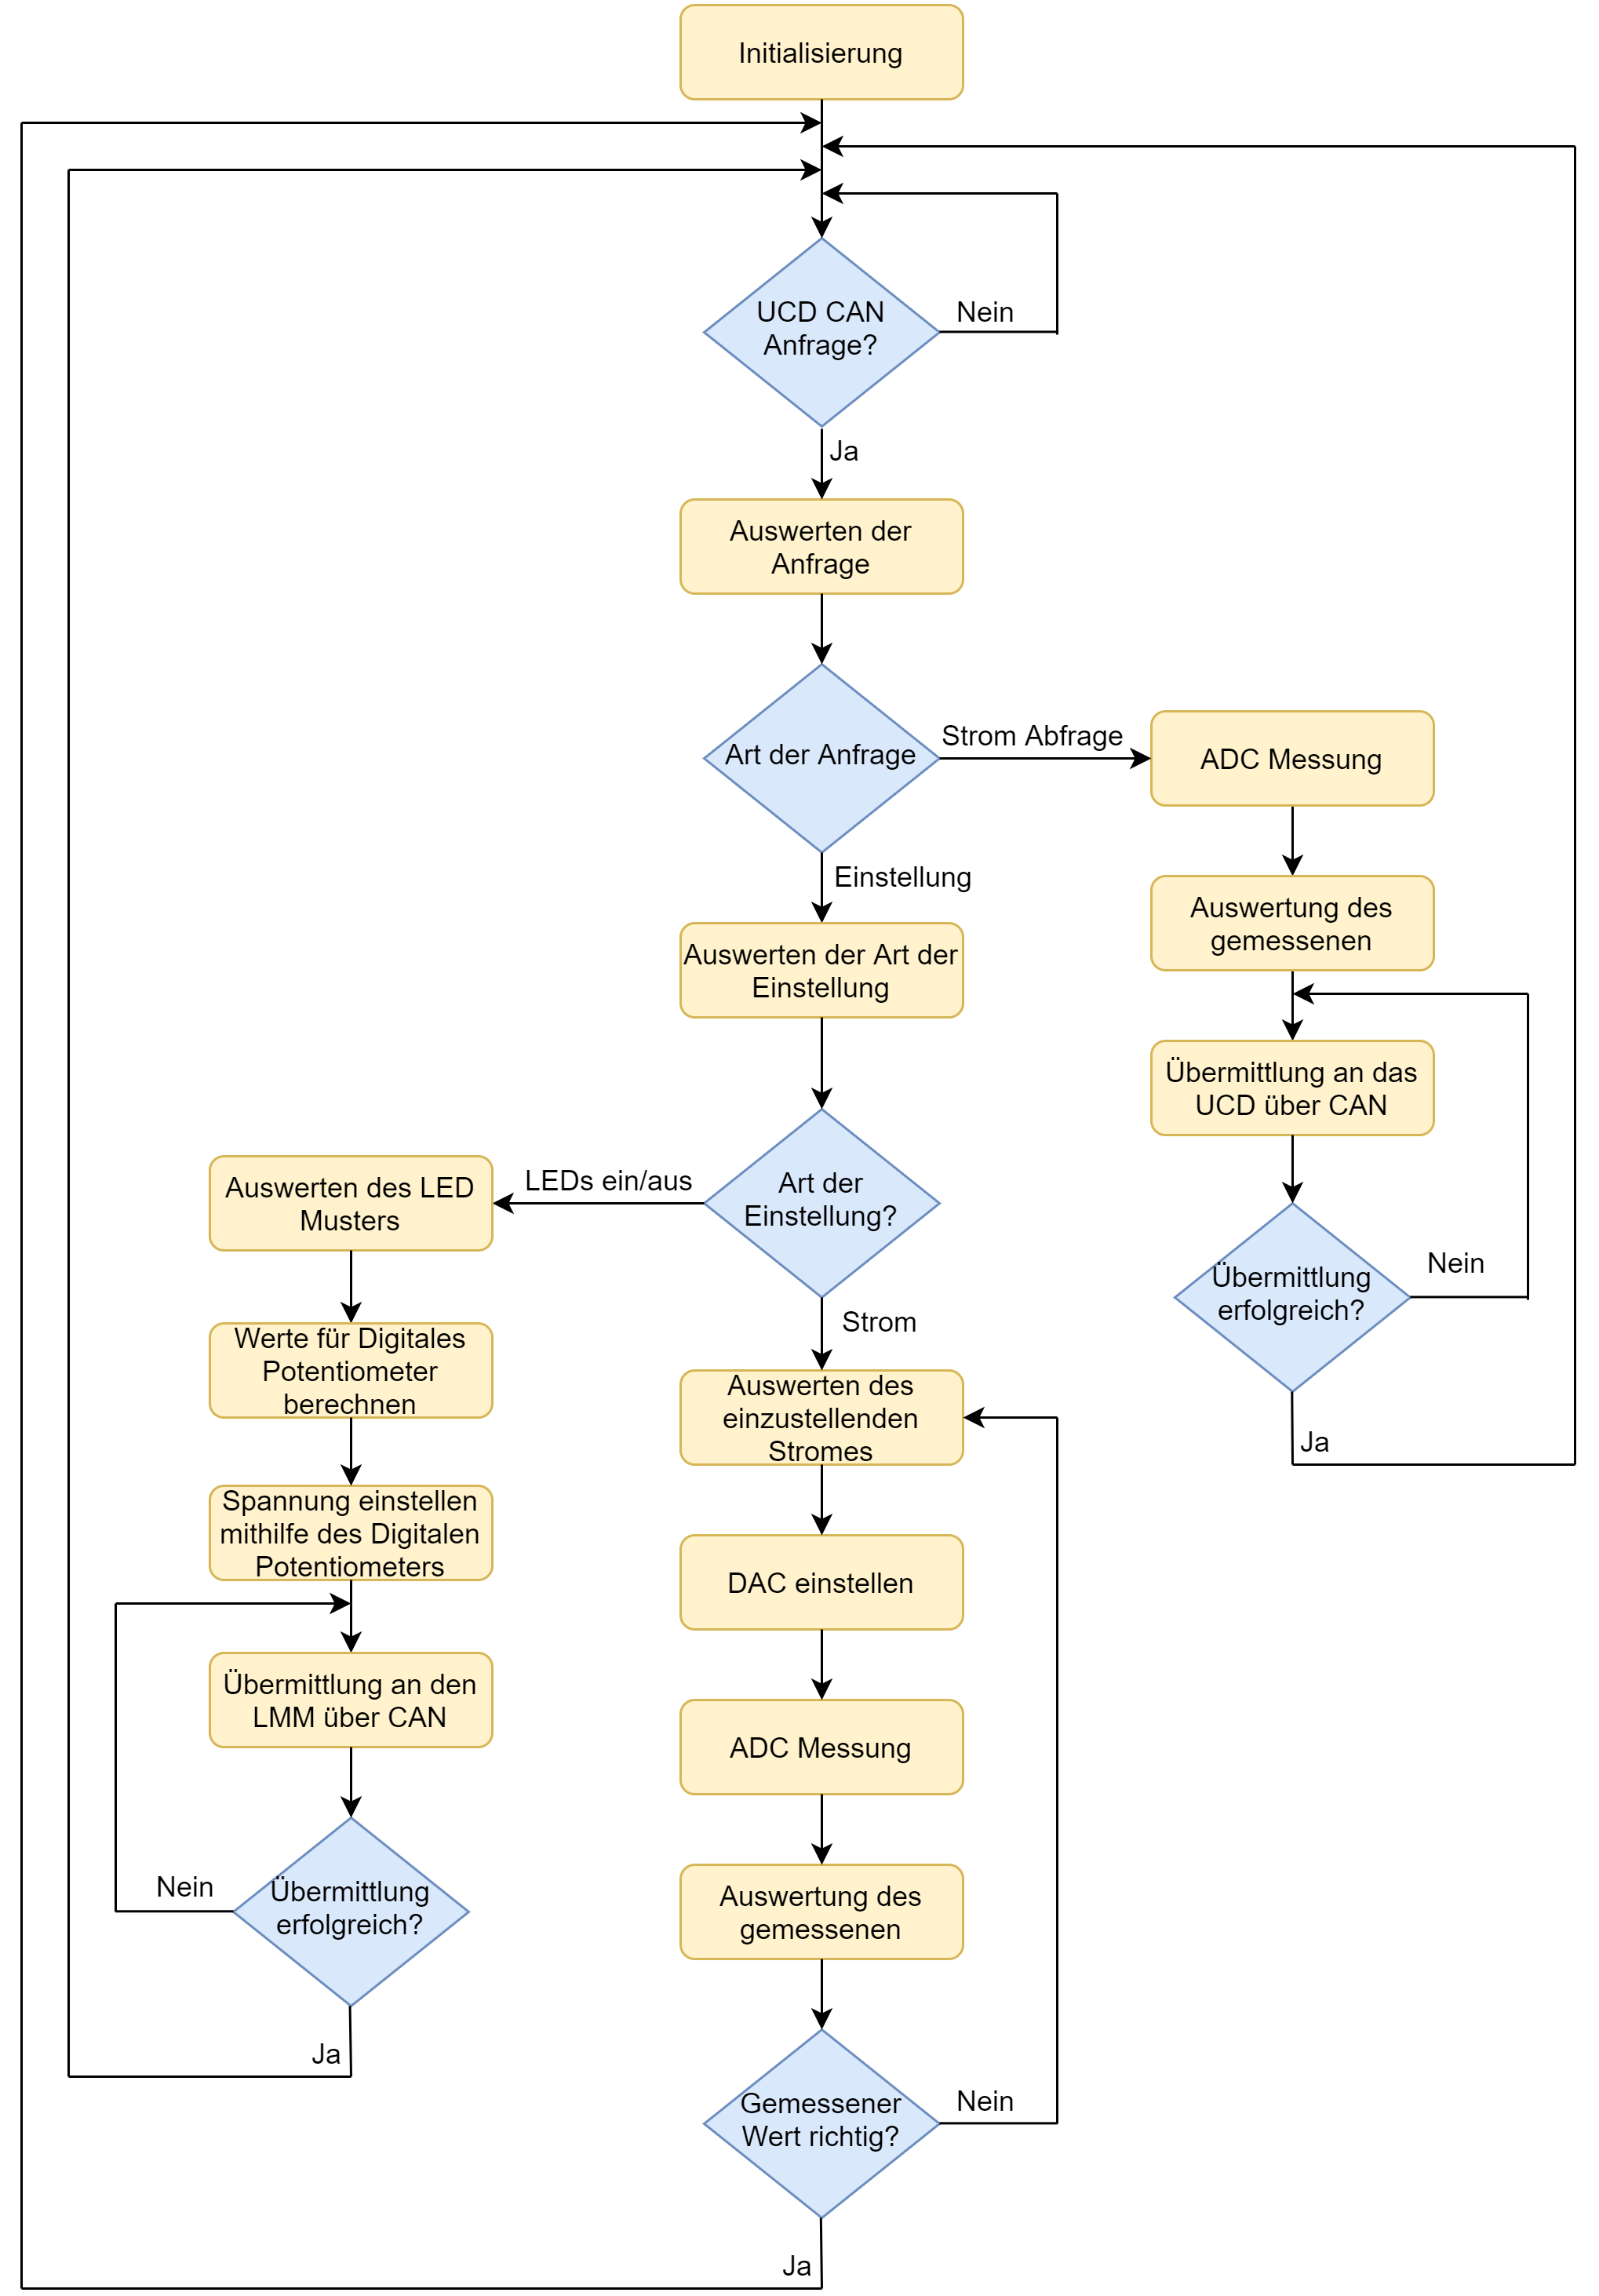
\includegraphics[height=18cm]{img/Dyn-LED-Driver-PAP.png}
		\end{adjustbox}
		Für noch besseres Verständnis der Abläufe im Programm folgt hier zusätzlich zum Programmablaufplan noch eine Detaillierte Erklärung der einzelnen Elemente davon. Oben angefangen und nach unten aufgearbeitet.
		\subsubsection{Initialisierung}\hfill \break
		Um die Gewünschte Funktionalität des Mikrocontrollers zu aktivieren, müssen vor dem eigentlichen Programmablauf alle Peripherie und auch interne Funktionen erst initialisiert werden. Dies wird mittels Bit schieben in den einzelnen Registern gemacht. \hfill \break \hfill \break		
		\textbf{Zu initialisierende Funktionen:}
		\begin{itemize}
			\item Controller Area Network
			\item Serial Peripheral Interface
			\item Analog Digital Converter
			\item Digital Analog Converter
		\end{itemize}
	
		\subsubsection{Ablauf}\hfill \break
		Nach der Initialisierung geht es direkt ins Hauptprogramm über, hier wird ständig überprüft, ob vom User Controlled Device eine Anfrage an den Mikrocontroller gemacht wurde. Hier gibt es zwei Möglichkeiten, entweder, eine Anfrage wurde getätigt, dann wird diese Ausgewertet. Ist aber keine Anfrage getätigt worden, beginnt es von neuem.\hfill \break \hfill \break
		Es gibt zwei mögliche Anfragen, die ausgewertet werden können. Diese sind die Abfrage des Stromes, der gerade gezogen wird und die Anweisung den Strom zu ändern oder LEDs ein oder auszuschalten.\hfill \break \hfill \break
		Soll der Strom gemessen werden, wird eine ADC Messung durchgeführt, die Ergebnisse davon werden dann ausgewertet und per CAN wieder an das User Controlled Device zurückgesendet.\hfill \break \hfill \break
		Beim Einstellen der LEDs wird ausgewertet, wie viele LEDs am Modul noch eingeschaltet sind, nach dem richtet sich die Spannung. Die Spannung wird durch das Verändern eines Spannungsteilers am Feedback Eingang des SEPIC Chips eingestellt. Dieser Spannungsteiler wird durch ein digitales Potentiometer verändert, es bekommt den Widerstand so eingestellt, dass die gewünschte Ausgangsspannung anliegt. Wie man auf die Werte kommt, kann im \hyperref[sec:berechnungen]{Kapitel Berechnungen} nachgelesen werden.\hfill \break \hfill \break
		Soll der Ausgangsstrom verändert werden, wird mithilfe des DACs die Spannung an einem der Operationsverstärker, die einen für den Stromfluss zuständigen MOSFET ansteuern, verändert. Nach dieser Änderung, wird eine ADC Messung durchgeführt, ob nun der richtige Strom fließt. Ist das nicht der Fall, wird überpüft ob zu viel oder zu wenig Strom fließt, nochmals mit dem DAC eingestellt und danach wieder gemessen, solange, bis der Wert stimmt. Sollte es gleich beim ersten Mal der gewünschte Wert sein, wird ganz von vorne begonnen und auf UCD Anfragen kommen.
		\newpage
		
		\subsection{Initialisierungen}\hfill \break
		\subsubsection{Initialisierung von CAN}\hfill \break
		Um CAN zu initialisieren, müssen pro CAN-Interface mindestens sechs Register beschrieben werden.
		Welche das sind, ist im Datenblatt zu finden, ab Seite 762. 
		Grundsätzlich sieht die CAN Initialisierung für diesen Anwendungsfall bei einem Interface wie folgt aus:
		\lstinputlisting[language=c, caption=C-Code für CANIF1 Initialisierung]{src/canInit.c}
		Im oben sichtbaren C-Code sieht man die Portpin Initialisierungen in den richtigen Modus. Weiters kann man sehen, wie die Konfiguration für diesen CAN Kanal durchgeführt wird. Im Letzten Bereich ist zu sehen, wie für diesen CAN Kanal einzelne Kontrollwerte eingestellt werden.
		Die wichtigsten Werte hier sind:
		\begin{itemize}
			\item Externer interrupt: aktiviert (wenn eine Übertragung stattfindet, wird diese sofort registriert)
			\item Overload handling: deaktiviert (wenn eine zu lange Übertragung festgestellt wird, wird nichts unternommen, da dies nicht vorkommen sollte)
			\item Anfragen auf den Kanal: aktiviert
		\end{itemize} 
		\newpage
		\subsubsection{Initialisierung von SPI}\hfill \break
		Für die Initialisierung von SPI müssen mindestens vier Register beschrieben werden. Diese können im Datenblatt ab Seite 657 aufgefunden werden.
		\lstinputlisting[language=c, caption=C-Code für SPI Initialisierung]{src/spiInit.c}
		Im C-Code über diesem Text sieht man, dass die GPIO-Pins auf Mode A, in diesem Fall der SPI Modus gesetzt wurden. Weiters wurde SPI im Master-Modus konfiguriert, das bedeutet der Mikrocontroller gibt die befehle und erhält keine. Das Anzusprechende gerät wird über einen Peripherie-Pin direkt ausgewählt.
		Die wichtigsten Werte hier sind:
		\begin{itemize}
			\item SPI-enable: aktiviert (SPI wird am Mikrocontroller aktiviert)
			\item Peripheral select: deaktiviert (Das gerät wird direkt angesprochen)
			\item Master-Modus: aktiviert
		\end{itemize} \newpage
		\subsubsection{Initialisierung vom DAC}\hfill \break
		Um den DAC zu initialisieren, müssen mindestens sechs Register beschrieben werden. Diese Register und weitere Möglichkeiten für Einstellungen sind im Datenblatt ab Seite 1148 zu finden. Für den hier benötigten Anwendungsfall sieht die Initialisierung wie folgt aus: 		 
		\lstinputlisting[language=c, caption=C-Code für DAC Initialisierung]{src/dacInit.c}
		Die wichtigsten Werte hier sind:
		\begin{itemize}
			\item Auto Refresh enable: aktiviert (DAC gleicht Abweichungen automatisch aus)
			\item Timer Register enable: deaktiviert (Nicht benötigt, da eine Konstante Spannung gewollt ist)
			\item Output enable: aktiviert
			\item DAC enable: aktiviert
		\end{itemize} \newpage
		\subsubsection{Initialisierung vom ADC}\hfill \break
		Um den ADC zu initialisieren, müssen mindestens dreizehn Register beschrieben werden. Diese Register und weitere Möglichkeiten für Einstellungen sind im Datenblatt ab Seite 1102 zu finden. Für den hier benötigten Anwendungsfall sieht die Initialisierung wie folgt aus: 		 
		\lstinputlisting[language=c, caption=C-Code für ADC Initialisierung]{src/adcInit.c}
		Die wichtigsten Werte hier sind:
		\begin{itemize}
			\item Timer start: aktiviert
			\item Timer stop: aktiviert 
			\item Sequencer Start of Conversion 0: aktiviert
			\item Muliplex Settle Time: aktiviert (Eineinhalb Fache zeit für den Multiplexer)
			\item External Reference: deaktiviert (Interne REferenzspannung wird für MEssung verwendet)
			\item Sample and Hold: aktiviert
			\item Reference Source: eins (Eingangsspannung)
			\item Freerunning mode: deaktiviert
			\item Single Sequencer Mode: aktiviert
			\item Sleep mode: deaktiviert
			\item ADC enable: aktiviert
		\end{itemize} \newpage
		
		\subsection{Controller Area Network}\hfill \break
			\subsubsection{Grundlagen zu CAN}\hfill \break
			Mit CAN werden mehrere gleichberechtigte Komponenten miteinander verbunden und können somit miteinander kommunizieren. Sehr beliebt ist es, wegen seiner Störsicherheit und der Echtzeitfähigkeit. Eingesetzt wird es häufig im Automobilbereich, und der Medizintechnik aber auch in vielen weiteren Systemen.
			
			Die Übertragung wird differenziell über zwei verdrillte Leitungen bewerkstelligt, dadurch wird die Störanfälligkeit minimiert. In folgender Grafik kann man sehen, wie diese bitweise Übertragung auf den beiden CAN Leitungen aussieht.
			\begin{adjustbox}{center,caption={CAN Übertragung},label={fig:CANbits.png},nofloat=figure,vspace=\bigskipamount}
				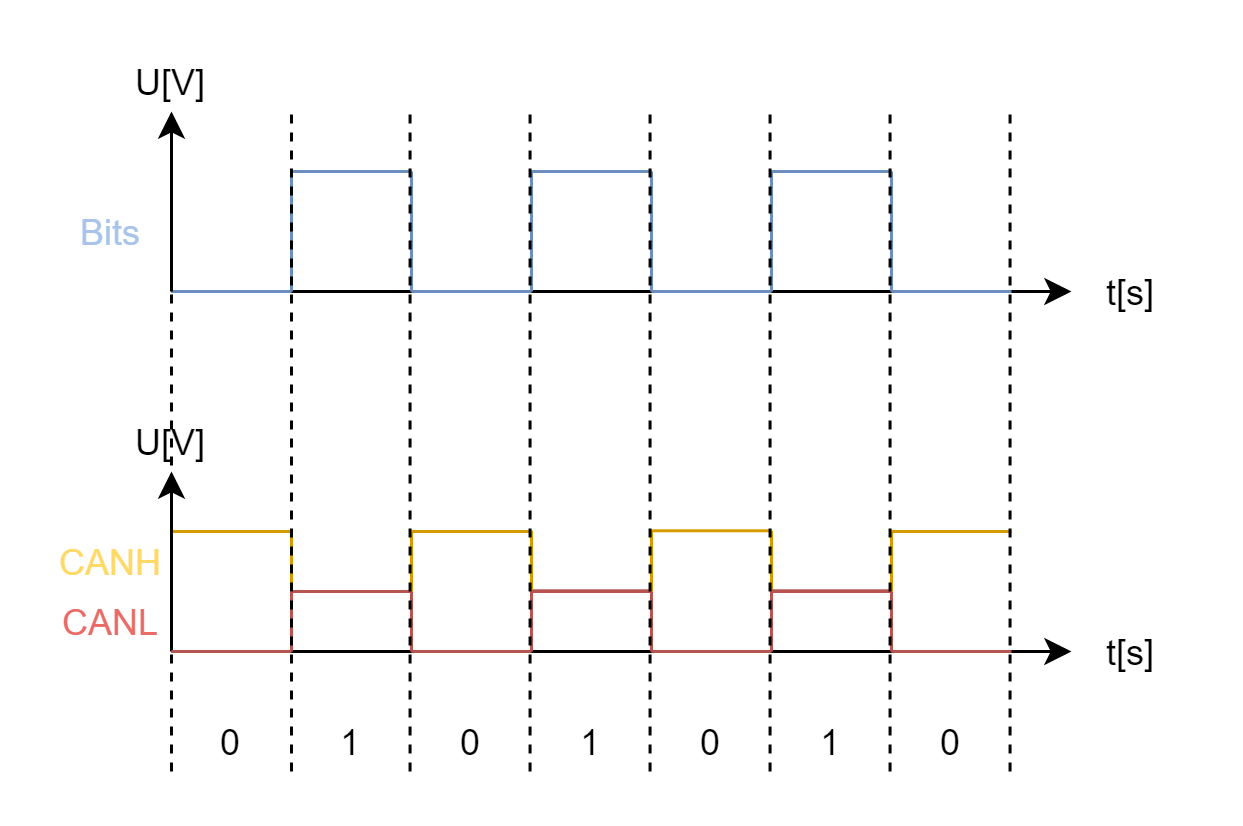
\includegraphics[width=\textwidth]{img/CAN_bits.png}
			\end{adjustbox}
		
			In diesem Fall wird Highspeed-CAN verwendet, was eine Übertragungsgeschwindigkeit von 1 Mbits/s ermöglicht.
			\newpage
			
			\subsubsection{LED Matrix Manager} \hfill \break
			Für die Kommunikation mit dem LMM sind einige Programmteile zuständig. Wie in einem vorherigen Kapitel schon beschrieben, auch die Initialisierungen. Hier werden aber hauptsächlich die Teile beschrieben, welche sich um das Zusammensetzen der Nachrichten des LMM kümmern. Zum einfachen Verständnis wird der Ablauf mittels Flussdiagramm dargestellt. \hfill \break
			\begin{adjustbox}{center,caption={Programmablauf LMM},label={fig:PABL-LMM},nofloat=figure,vspace=\bigskipamount}
				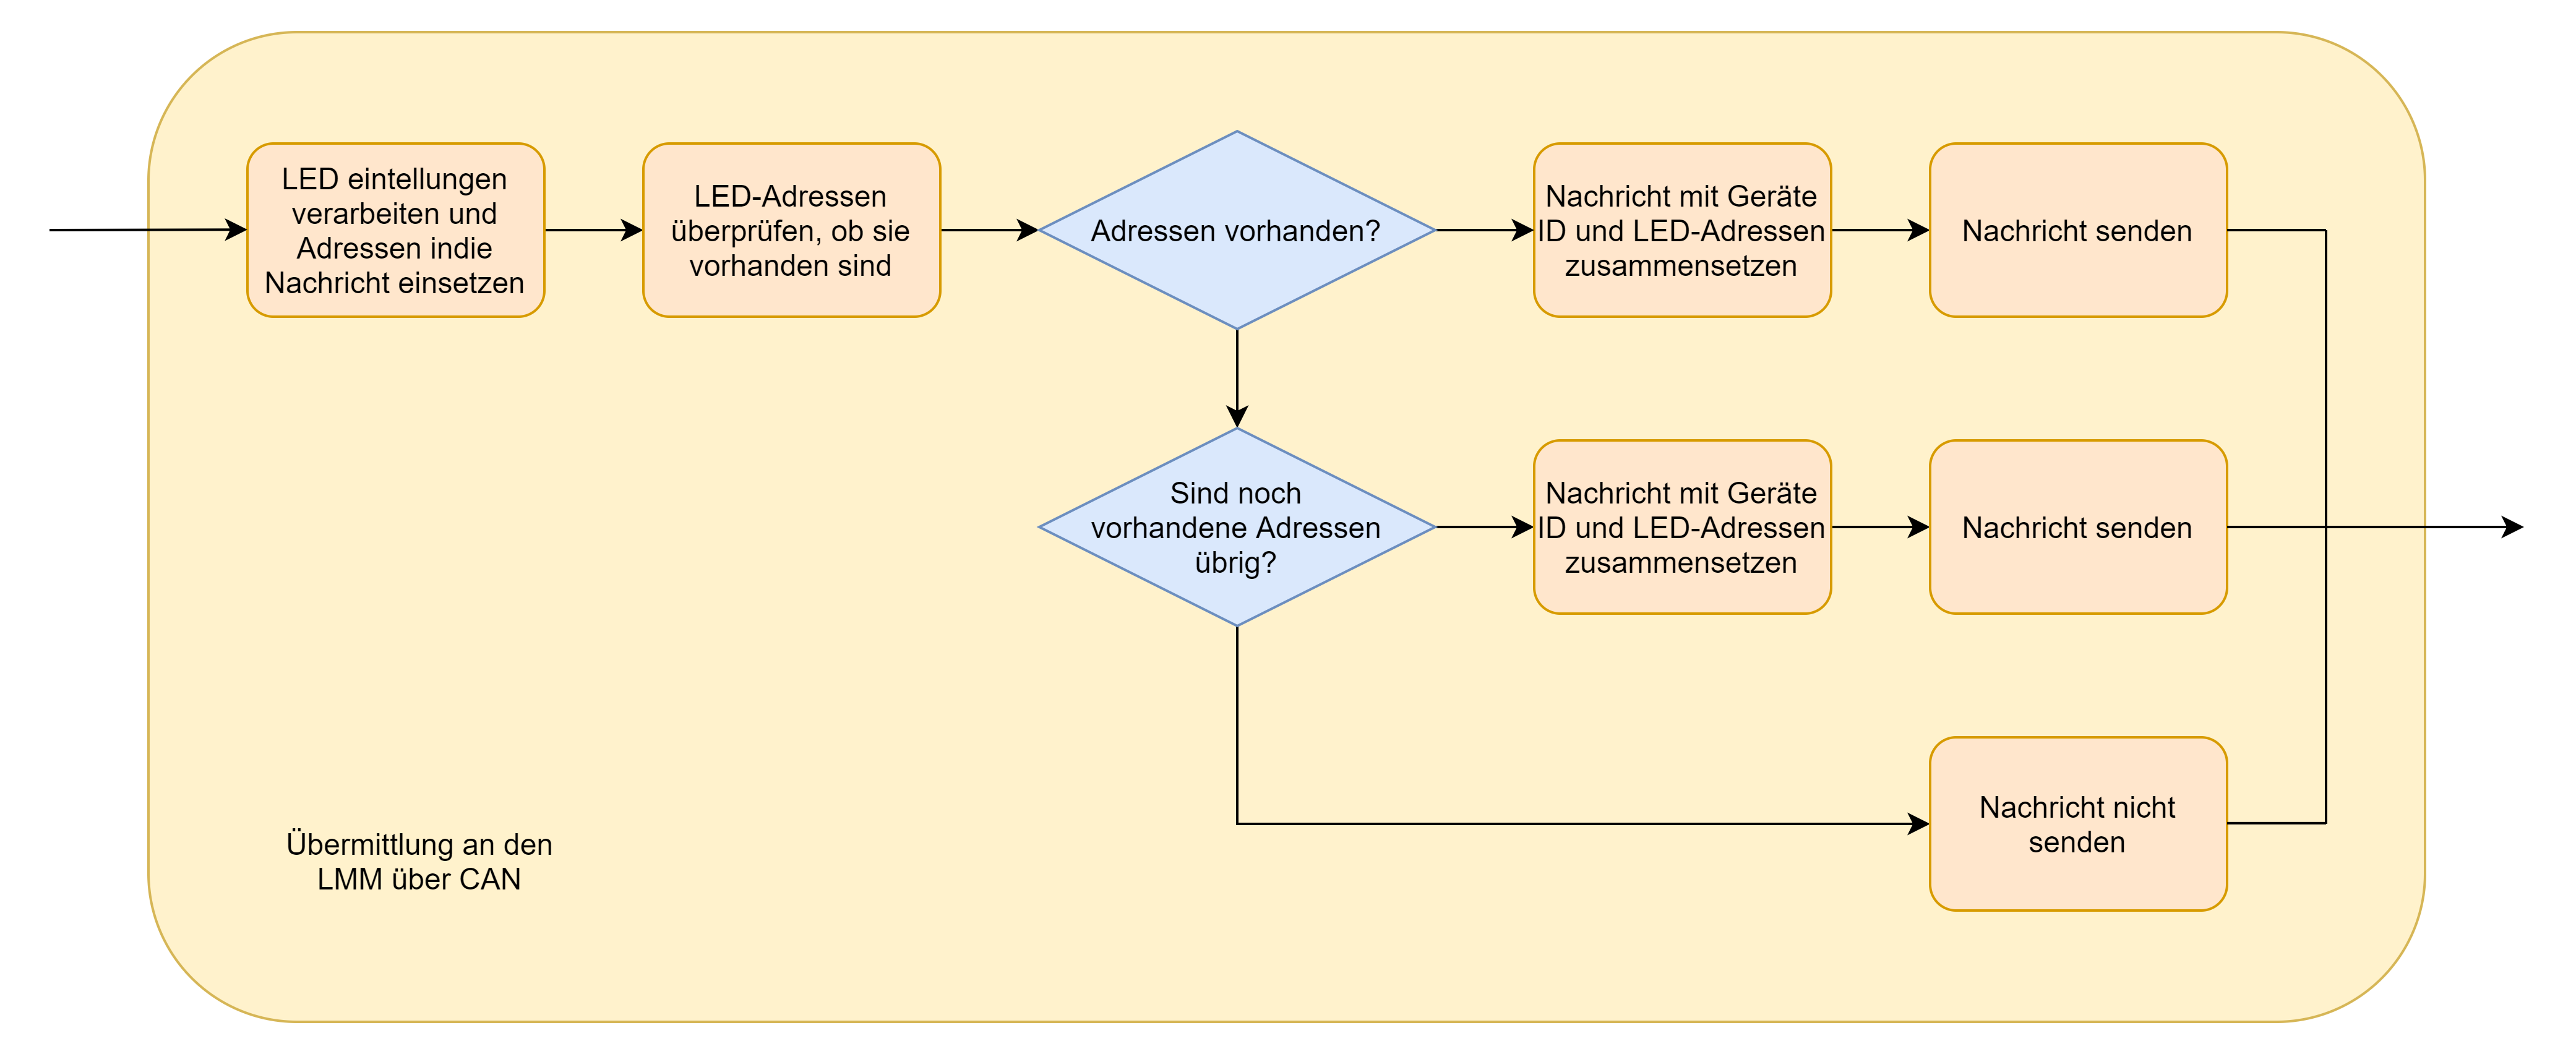
\includegraphics[width=\textwidth]{img/Programmablauf-LMM.png}
			\end{adjustbox} \hfill \break
			Im Programmablauf ist der Teil des Programmablaufplans von Abbildung \ref{fig:PAP.png}, mit der Bezeichnung 'Übermittlung an den LMM über CAN' zu sehen. Bei diesem Prozess gibt es drei verschiedene Möglichkeiten, wie die Übertragung stattfindet, beziehungsweise ob sie stattfindet. Im Grunde werden einer Funktion alle Daten, also die ein oder auszuschaltenden LED-Adressen übergeben. Diese Adressen werden dann zu einer Nachricht zusammengesetzt, also dass nicht viele einzelne Adressen hintereinander geschickt werden, sondern mehrere gleichzeitig. Im nächsten Schritt wird überprüft ob die verwendeten Adressen in den Vordefinierten Adressen enthalten sind. \hfill \break \newpage
			\textbf{Die Vordefinierten Adressen sehen wie folgt aus:} \hfill \break
			\lstinputlisting[language=c, caption=LED Adressen des LMMs]{src/LEDAdressen.c} \hfill \break
			Um diese Adressen mit den Eingegangenen zu vergleichen wird eine Schleife verwendet, die jede eingegangene Adresse einzeln mit jeder Vordefinierten Adresse vergleicht. Passen alle Adressen wird eine Nachricht mit LMM-ID und den zu toggelnden LEDs zusammengesetzt und diese wird im Anschluss versendet. \hfill \break \hfill \break
			Stimmen nicht alle Adressen, werden die falschen weggelassen und nur die Korrekten werden in das Adressen, ID Paket eingefügt, im Anschluss wird die Nachricht dann versendet. \hfill \break \hfill \break
			Sollten keine der Adressen stimmen, wird gar keine CAN-Nachricht versendet, da es ja auch keine Veränderung am LMM bringen würde.
			\newpage
			
		\ifoot{Dominik Gansch}
		\subsection{Serial Peripheral Interface}\hfill \break
			Das Digitale-Potentiometer benutzt SPI zur Datenübertragung zwischen dem Mikrocontroller.
			\subsubsection{Digitales Potentiometer}
			Als Digitales Potentiometer wurde das MCP4251 von Microchip verwendet.\hfill \break
			\begin{adjustbox}{center,caption={MCP4251},label={fig:MCP4251},nofloat=figure,vspace=\bigskipamount}
				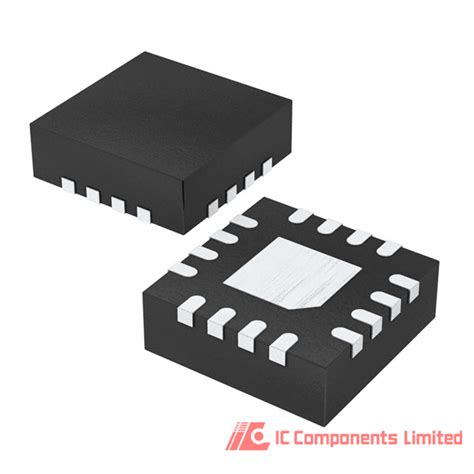
\includegraphics[width=\textwidth]{img/MCP4251.jpg}
			\end{adjustbox} \hfill \break
			\newpage
	%	\subsection{Digital Analog Converter}\hfill \break
		%	\subsubsection{Grundlagen zum DAC}\hfill \break
	%		\newpage
	%	\subsection{Analog Digital Converter}\hfill \break
	%		\subsubsection{Grundlagen zum ADC}\hfill \break
	%		\newpage
\ifoot{Florian Hintermeier}	
\chapter{Betriebswirtschaftliche Kalkulation}\hfill \break
Die Betriebswirtschaftliche Kalkulation dient der Übersicht der Kosten in einem Unternehmen oder wie in diesem Fall einem Projekt. Hier werden die Berechnungen so aufgestellt, als würde dieses Projekt von einem Kleinunternehmen hergestellt werden. 
	\section{Kostenrechnung}\hfill \break
		\subsection{Personalkosten und Arbeitszeit}\hfill \break
		Ein großer Kostenpunkt sind Personalkosten, die je nach Abschluss, Erfahrung und auch Arbeitszeit des Mitarbeiters unterschiedlich sein können.
		Durchschnittlich verdienen HTL Absolventen 28130€ im Jahr, das ist bei einer Anstellung mit 38,5 Stunden in der Woche ein Stundenlohn von 13,05€. \footnote{https://www.absolventen.at/magazin/gehaltsvorstellung-was-ist-deine-leistung-wert/}
		\begin{align*} 
		K_{ P } = 13,05\text{€/h} * (349,3\text{h} + 342,3\text{h}) = 9025,38\text{€}
		\end{align*} 
		\subsection{Arbeitsplatz}\hfill \break
		Die Mietpreise für Büroimmobilien liegen in Österreich durchschnittlich bei 11,5€/m².\footnote{https://www.brainpower-austria.at/bueromieten-in-wien-mit-diesen-quadratmeterpreisen-muessen-sie-rechnen/} Da zwei Personen an diesem Projekt arbeiten, wird eine Immobilie mit 25m² gemietet. Mit einer Arbeitszeit von etwas über zwei Monaten, hierfür werden drei gerechnet, da man normalerweise ganze Monate mietet, ergeben sich folgende Mietkosten:
		\begin{align*} 
		K_{ A } = 25\text{m²} * 11,5\text{€/m²} * 3\text{Monate} = 862,5\text{€}
		\end{align*} 
		\subsection{Ausrüstung}\hfill \break
		Diese Geräte werden für die Herstellung und Messungen benötigt:
		\begin{itemize}
			\item EDUX1002A - Oszilloskop, 2x 50MHz, 1GSPS, Keysight - 561,60€\footnote{https://www.distrelec.at/de/oszilloskop-2x-50mhz-1gsps-keysight-edux1002a/p/30081607}
			\item RND 560-00155 - Lötstation 100W 500°C 230V, RND Lab - 186,84€\footnote{https://www.distrelec.at/de/loetstation-100w-500-230v-rnd-lab-rnd-560-00155/p/30088279}
		\end{itemize}
		Das sind in Summe 748,44€.
		\newpage
		
		\subsection{Produktionskosten}\hfill \break
		Zu den Produktionskosten gehören, die Bauteile, die PCBs und auch die Verschleißteile wie Lötzinn.
		\begin{itemize}
			\item Bauteile - 82,62€
			\item PCB - 24,60€\footnote{https://www.allpcb.com/}
			\item Lötzinnrolle - 11,49€\footnote{https://www.obi.at/loetzubehoer/loetzinnrolle/p/2298420}
		\end{itemize}
		Gesamt sind das 118,71€.
		
		\subsection{Gesamtkosten}\hfill \break
		\begin{itemize}
			\item Personalkosten - 9025,38€
			\item Arbeitsplatzkosten - 862,5€
			\item Ausrüstungskosten - 748,44€
			\item Produktionskosten - 118,71€
		\end{itemize}
		\textbf{SUMME: 10755,03€}
		\newpage	
	
	\section{Break-Even-Analyse}\hfill \break
		\subsection{Break-Even-Point}\hfill \break
		\begin{align*} 
		Break-Even-Point = \frac{Investitionskosten}{Deckungsbeitrag}
		\end{align*} 
		\begin{align*} 
		Investitionskosten = Personalkosten + Arbeitsplatzkosten + Ausrüstungskosten
		\end{align*} 
		\begin{align*} 
		Investitionskosten = 9025,38\text{€} + 862,5\text{€} + 748,44\text{€} = 10636,32\text{€}
		\end{align*} 
		\begin{align*} 
		Deckungsbeitrag = \text{Erlöse} - Produktionskosten
		\end{align*} 
		\begin{align*}
		Deckungsbeitrag = 200\text{€} - 118,71\text{€} = 81,29\text{€}
		\end{align*} 
		\begin{align*} 
		Break-Even-Point = \frac{10636,32\text{€}}{81,29\text{€}} = \text{130,84 also \textbf{131 Stück}}
		\end{align*} 
		\begin{adjustbox}{center,caption={Brek-Even-Point},label={fig:BEP.PNG},nofloat=figure,vspace=\bigskipamount}
			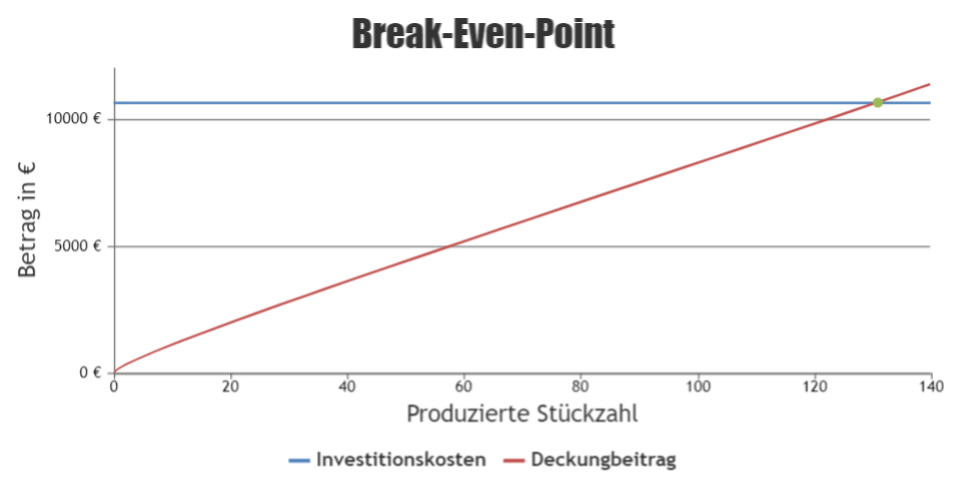
\includegraphics[width=\textwidth]{img/BEP.PNG}
		\end{adjustbox}
			
		\subsection{Break-Even-Umsatz}\hfill \break
		\begin{align*} 
		Break-Even-Umsatz = Break-Even-Point * Erlöse
		\end{align*} 
		\begin{align*} 
		Break-Even-Umsatz = 131 \text{Stück} * 200\text{€} = 26200\text{€}
		\end{align*} 
\newpage
			



\ifoot{Florian Hintermeier, Dominik Gansch}
%% ANHANG ==============================================%%
\appendix

%% abkürzungsverzeichnis ===============================%%
%% start of file abkuerzungen.tex

% Abkuerzungsverzeichnis
\addchap{
	\iflanguage{english}{Acronyms}{Abkürzungsverzeichnis}}
\begin{acronym}[ACRONYM]
\acro{adc}[ADC]{Analog Digital Converter}
\acro{can}[CAN]{Controller Area Network}
\acro{dac}[DAC]{Digital Analog Converter}
\acro{ldo}[LDO]{Low-Dropout regulator}
\acro{lmm}[LMM]{LED Matrix Manager}
\acro{pcb}[PCB]{Printed Circuit Board}
\acro{sepic}[SEPIC]{Single Ended Primary Inductance Converter}
\acro{opv}[OPV]{Operationsverstärker}
\acro{fet}[FET]{Field-Effect Transistor}
\acro{led}[LED]{Light Emitting Diode}
\acro{z-diode}[Z-Diode]{Zener Diode}
\acro{r}[R]{Resistor}
\acro{c}[C]{Capacitor}
\acro{gper}[GPER]{General Purpose Enable Register}
\acro{canif}[CANIF]{Control Area Network Interface}
\acro{cancfg}[CANCFG]{Control Area Network Configuration}
\acro{canctrl}[CANCTRL]{Control Area Network Controll}
\acro{mbits}[Mbit/s]{Megabit pro Sekunde}
\acro{mosi}[MOSI]{Master Out Slave In}
\acro{miso}[MISO]{Master In Slave Out}
\acro{sda}[SDA]{Serial Data Out}
\acro{sdi}[SDI]{Serial Data In}
\acro{ucd}[UCD]{User Controlled Device}
\acro{led}[LED]{Light Emitting Diode}
\acro{mosfet}[MOSFET]{Metal–Oxide–semiconductor Field-Fffect Transistor}
\acro{fet}[FET]{Field-Fffect Transistor}
\acro{gpio}[GPIO]{General Purpose In Out}
\acro{i/o}[I/O]{In/Out}
\acro{tdr}[TDR]{Transmit Data Register}
\end{acronym}\newpage

%% end of file abkuerzungen.tex
%%======================================================%%

%% abbildungsverzeichnis ===============================%%
\setcounter{lofdepth}{2}
\dipalistoffigures
%%======================================================%%

%% listingsverzeichnis =================================%%
\newpage
\addcontentsline{toc}{chapter}{Listings}\lstlistoflistings
%%======================================================%%

%% tabellenverzeichnis =================================%%
%\setcounter{lotdepth}{2}
%\dipalistoftables
%%======================================================%%

%% literaturverzeichnis ================================%%
%%\newewpage
%%\begin{literature}
% The TeXbook by D. E. Knuth
\bibitem[1]{TeXbooooook}{\textbf{Donald~E.~Knuth:} \emph{The \TeX{}book}. 1986, {\scshape Addison--Wesley} Verlag,\\ ISBN-13: 978-0-201-13447-6}

\end{literature}
 
%%======================================================%%

%% Zeitaufzeichnungen Hintermeier ======================%%
\newpage
\ifoot{Florian Hintermeier}
\markright{Zeitaufzeichnungen Hintermeier}
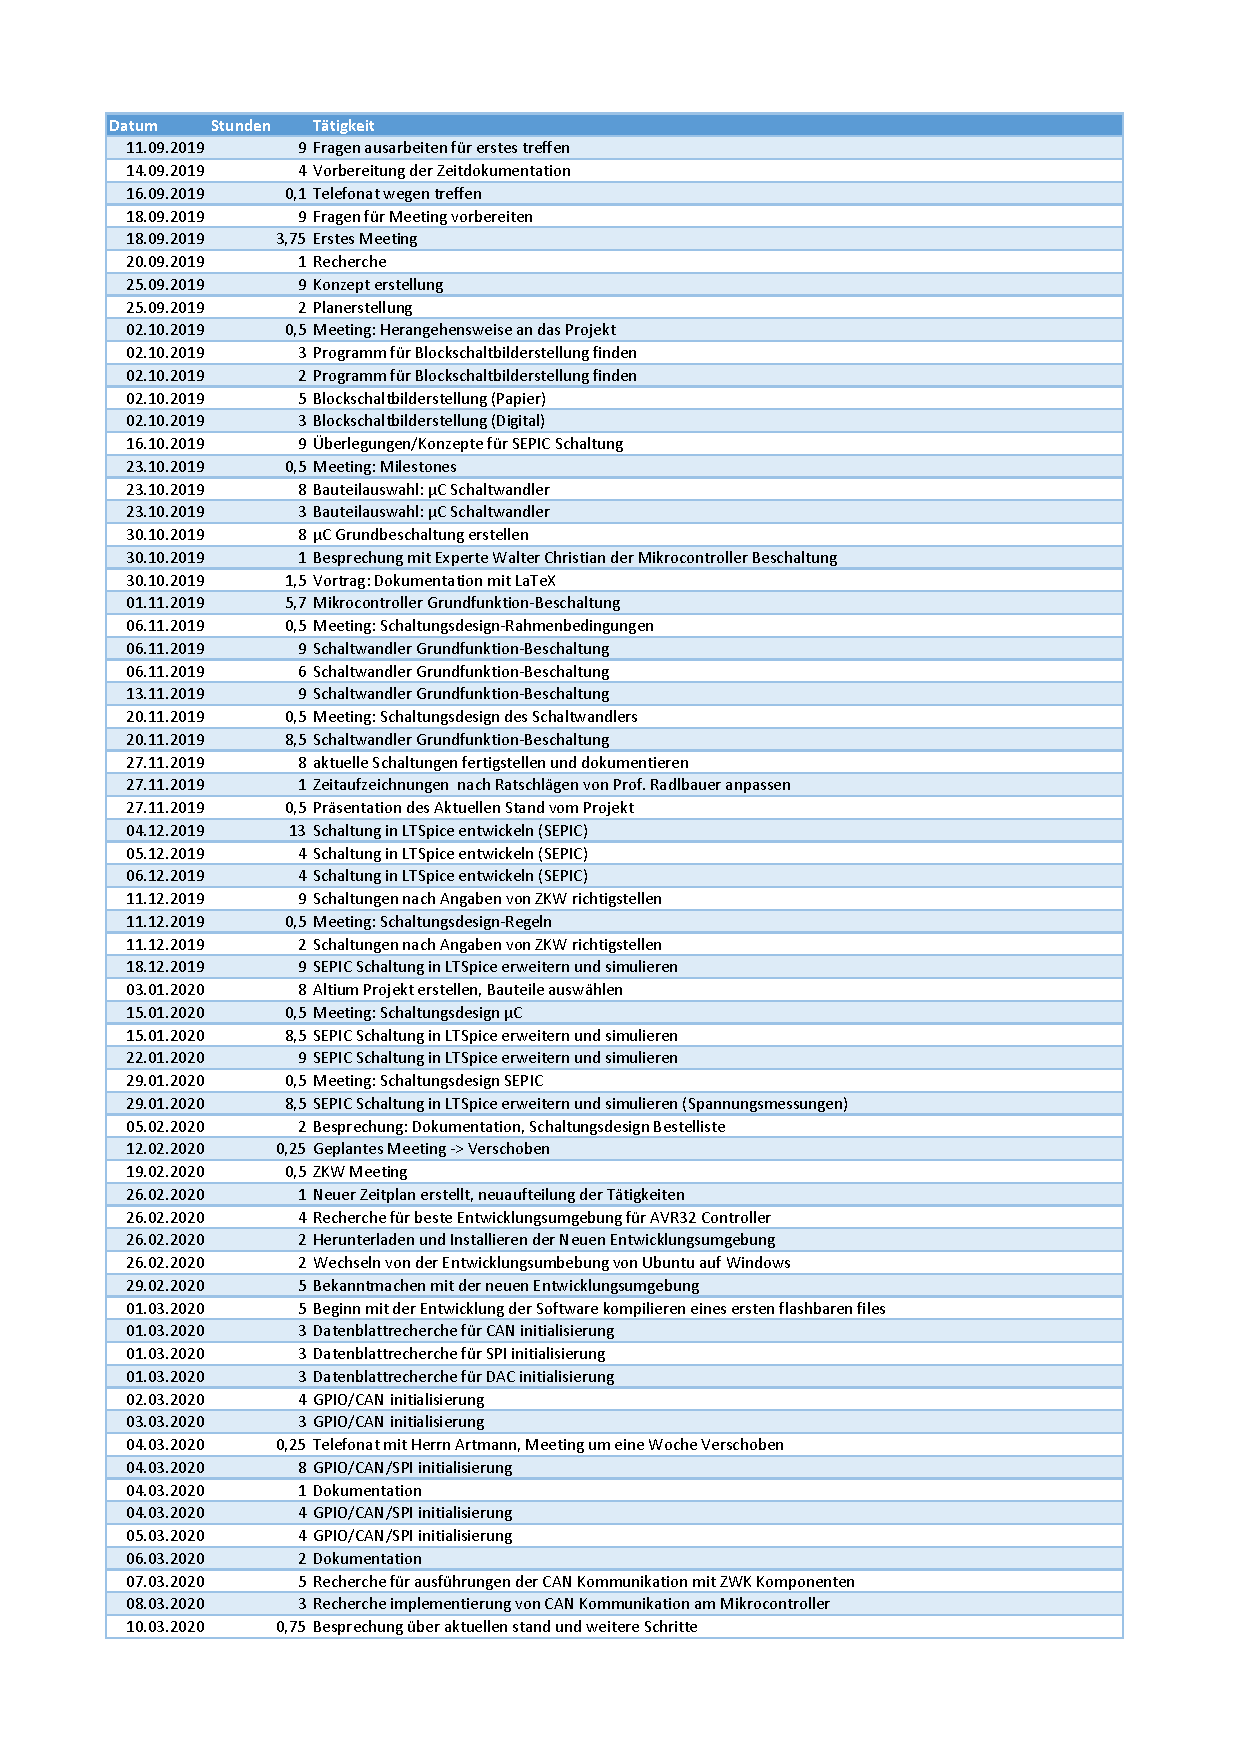
\includepdf[pages=1, pagecommand={\phantomsection\addcontentsline{toc}{chapter}{Zeitaufzeichnungen Hintermeier}}]{form/Zeit_hintermeier.pdf}
\includepdf[pages=2, pagecommand={\phantomsection}]{form/Zeit_hintermeier.pdf}
%%======================================================%%

%% Zeitaufzeichnungen Gansch ===========================%%
\newpage
\ifoot{Dominik Gansch}
\markright{Zeitaufzeichnungen Gansch}
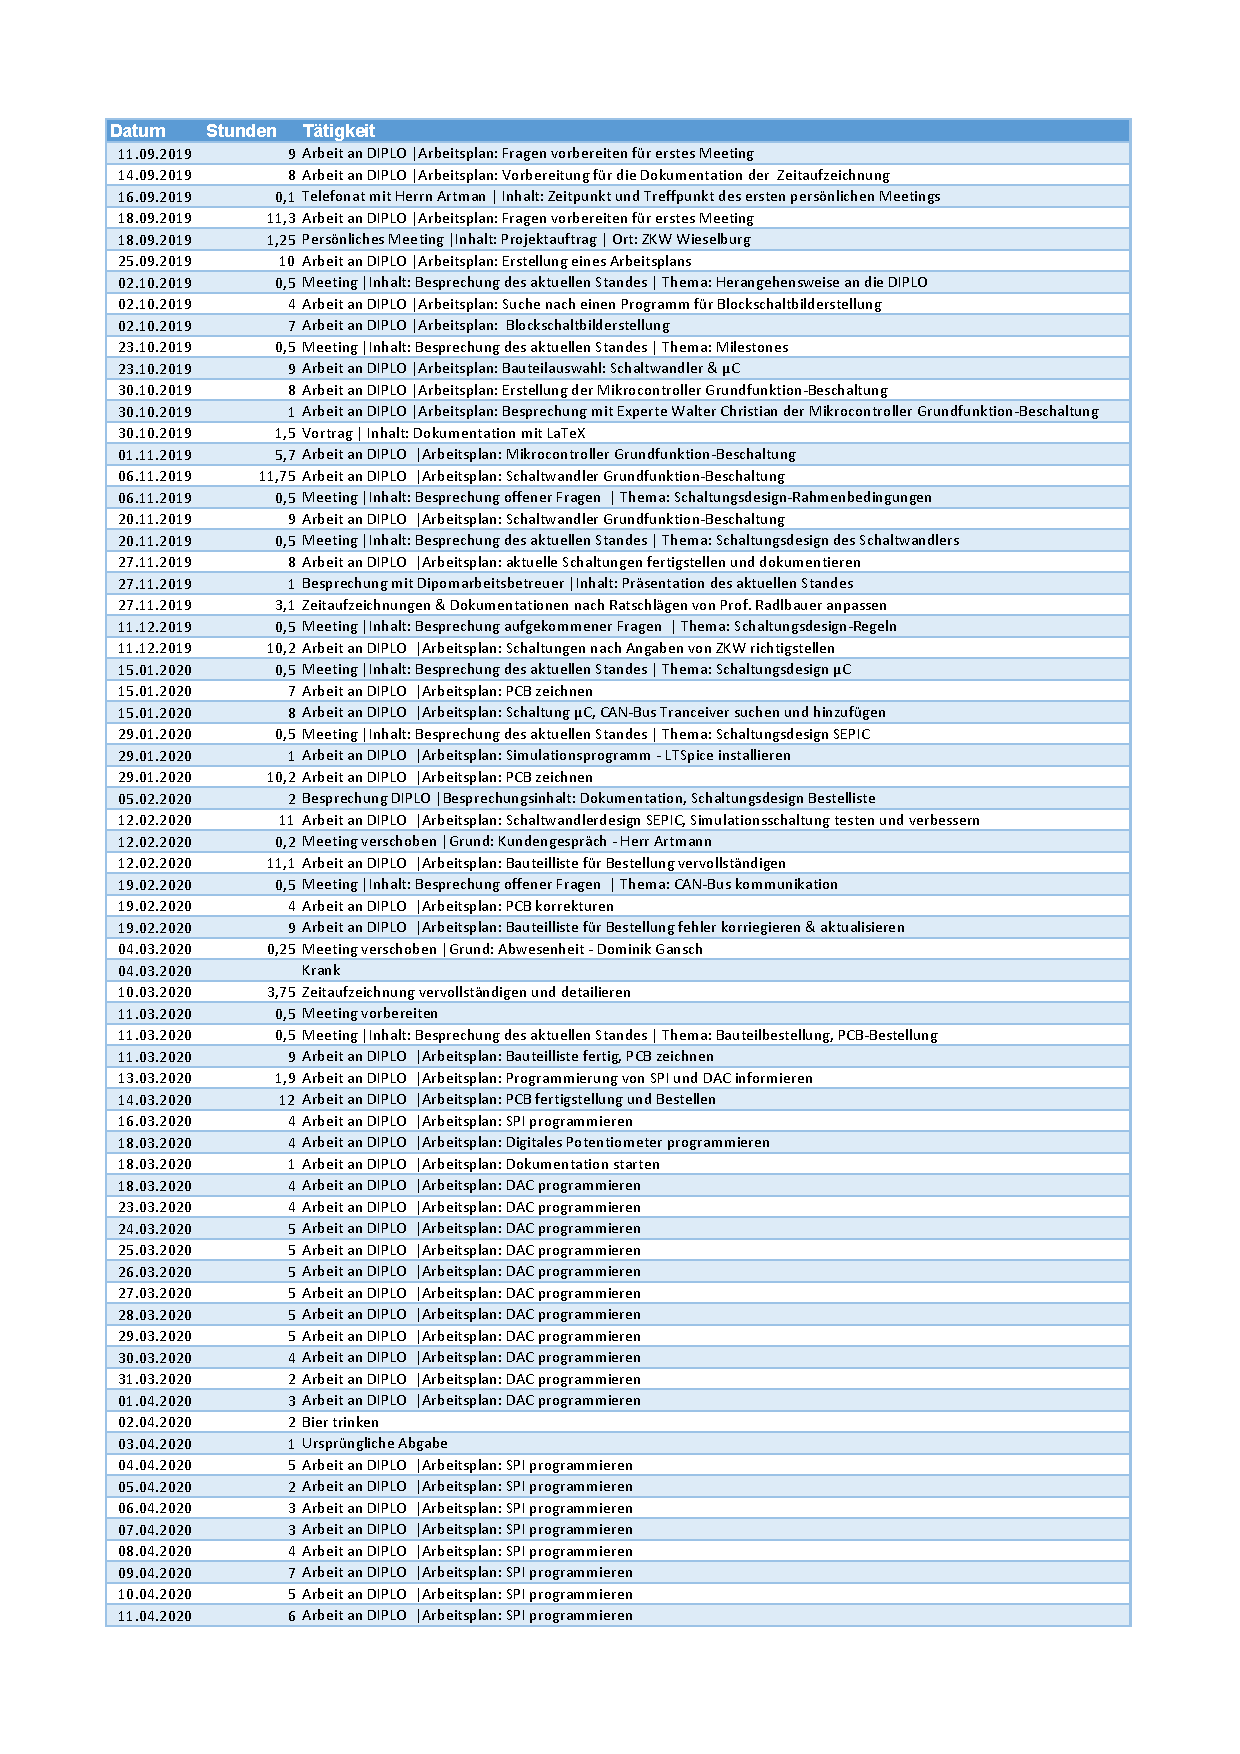
\includepdf[pages=1, pagecommand={\phantomsection\addcontentsline{toc}{chapter}{Zeitaufzeichnungen Gansch}}]{form/Zeit_gansch.pdf}
\includepdf[pages=2, pagecommand={\phantomsection}]{form/Zeit_gansch.pdf}
%%======================================================%%

\newpage
\markright{Schaltung Digitalteil}
\ifoot{Dominik Gansch}
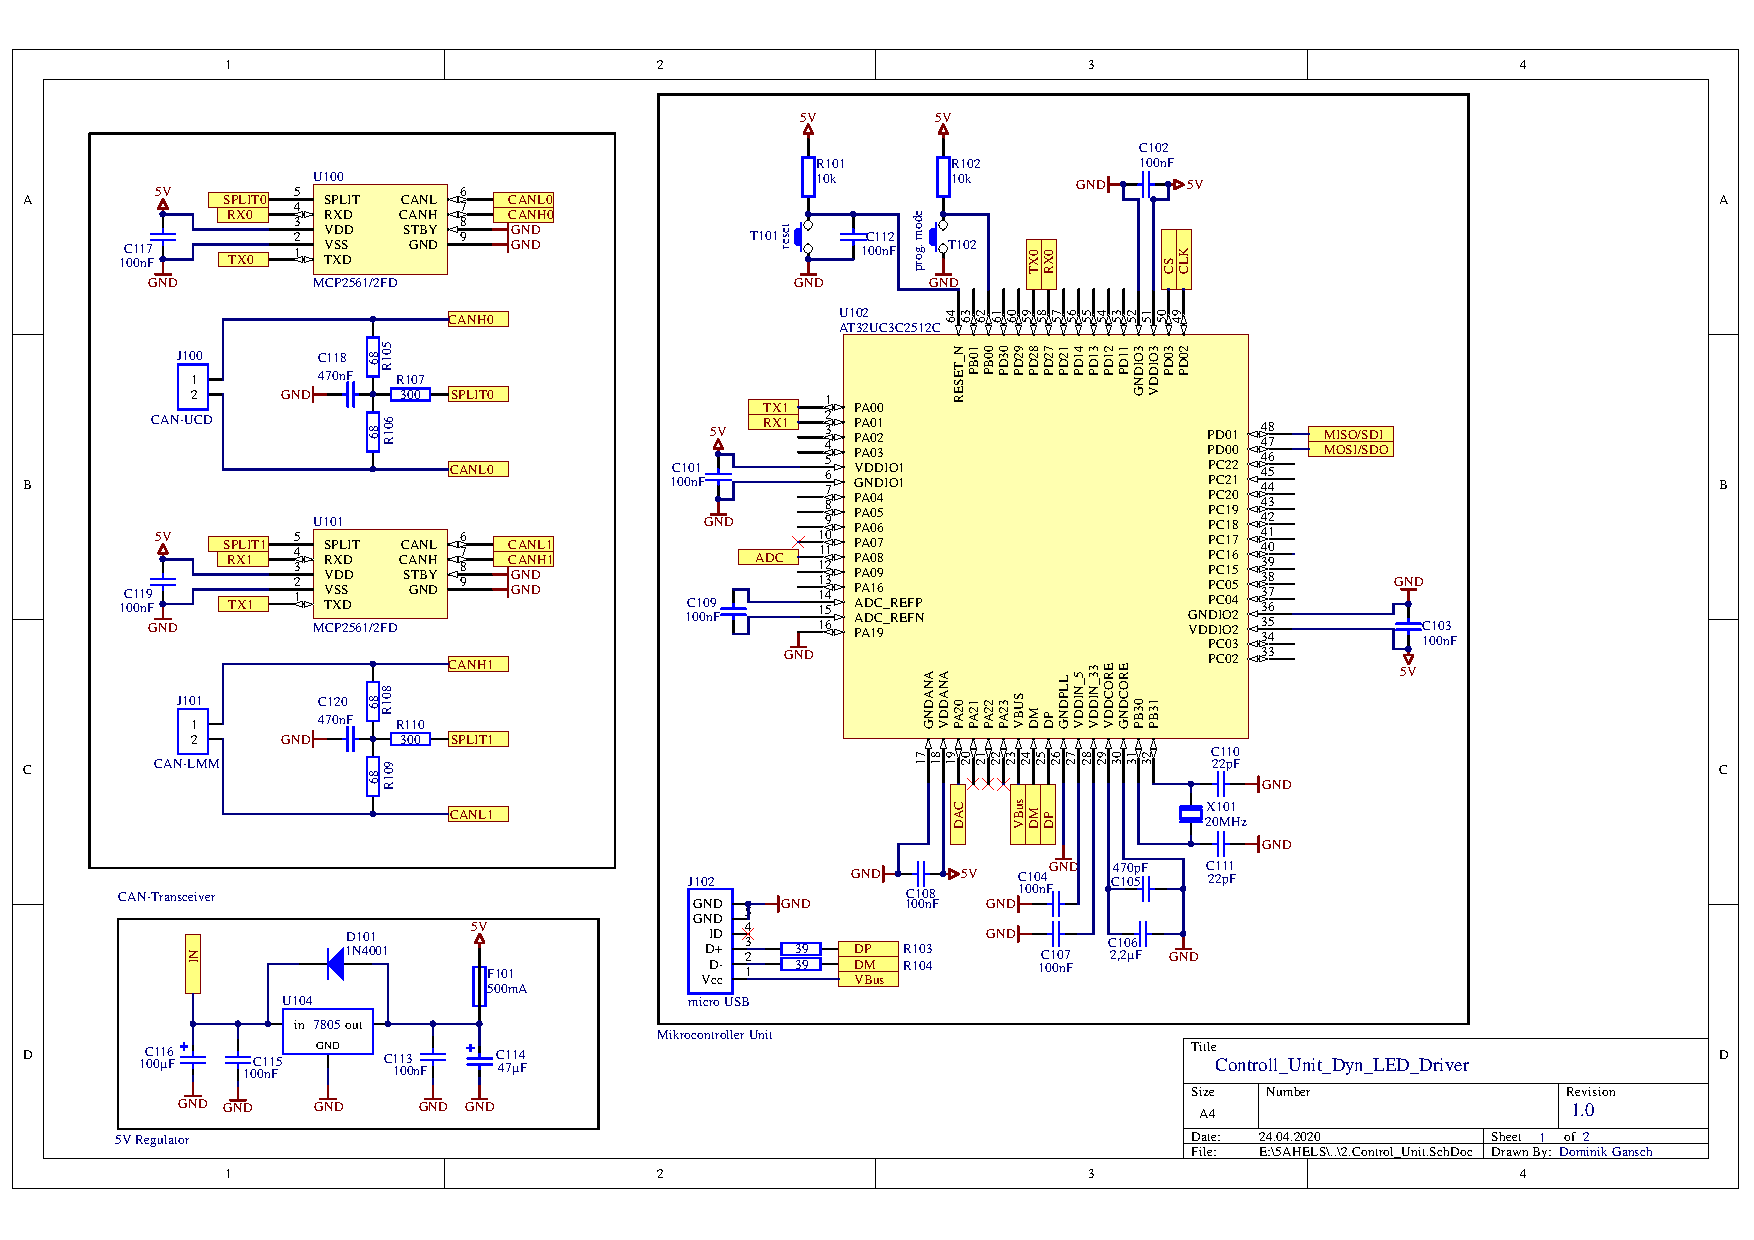
\includepdf[pages=1,angle=90, scale=0.9, pagecommand={\phantomsection\addcontentsline{toc}{chapter}{Schaltung Digitalteil}}]{schaltungen/Dynamic_LED_Driver.pdf}
\newpage
\markright{Schaltung Analogteil}
\ifoot{Florian Hintermeier}
\includepdf[pages=2,angle=90, scale=0.9, pagecommand={\phantomsection\addcontentsline{toc}{chapter}{Schaltung Analogteil}}]{schaltungen/Dynamic_LED_Driver.pdf}
\newpage
\markright{Bauteilliste}
\ifoot{Florian Hintermeier, Dominik Gansch}
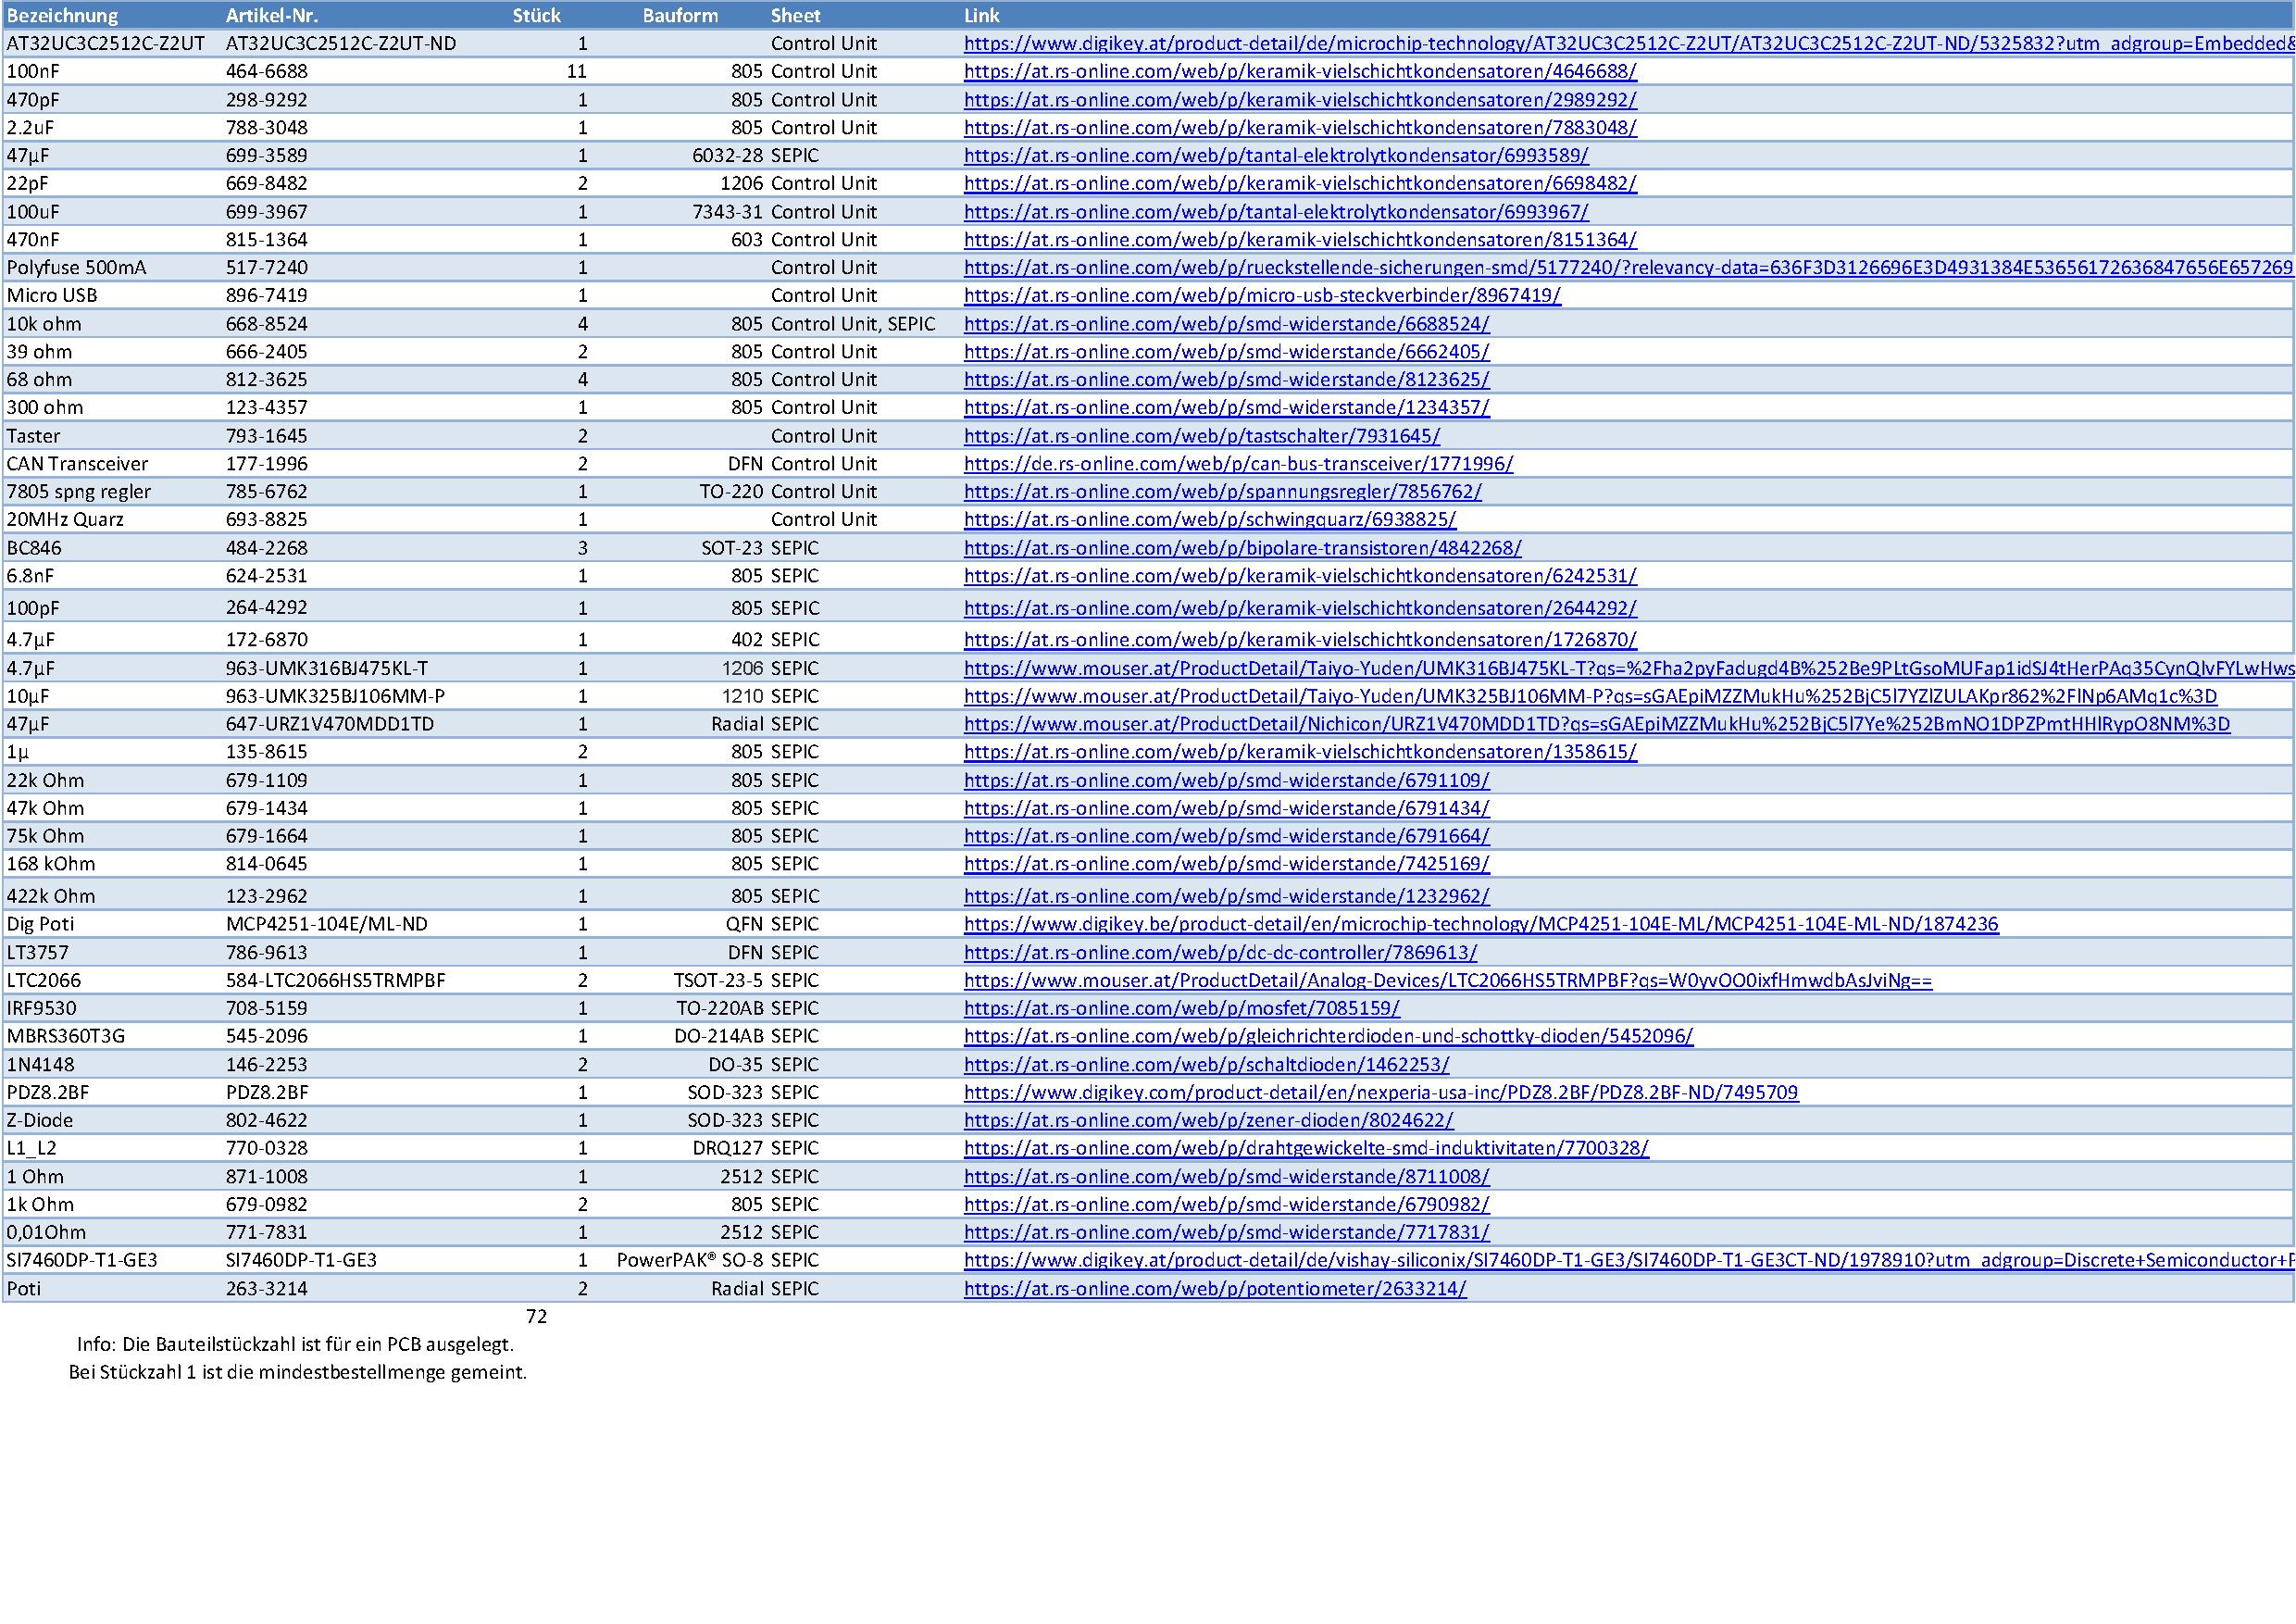
\includepdf[pages=-,angle=90, scale=0.9, pagecommand={\phantomsection\addcontentsline{toc}{chapter}{Bauteilliste}}]{schaltungen/Bauteilliste.pdf}

%% betreuungsprotokolle ================================%%
\newpage
\markright{Diplomarbeit Seminare}
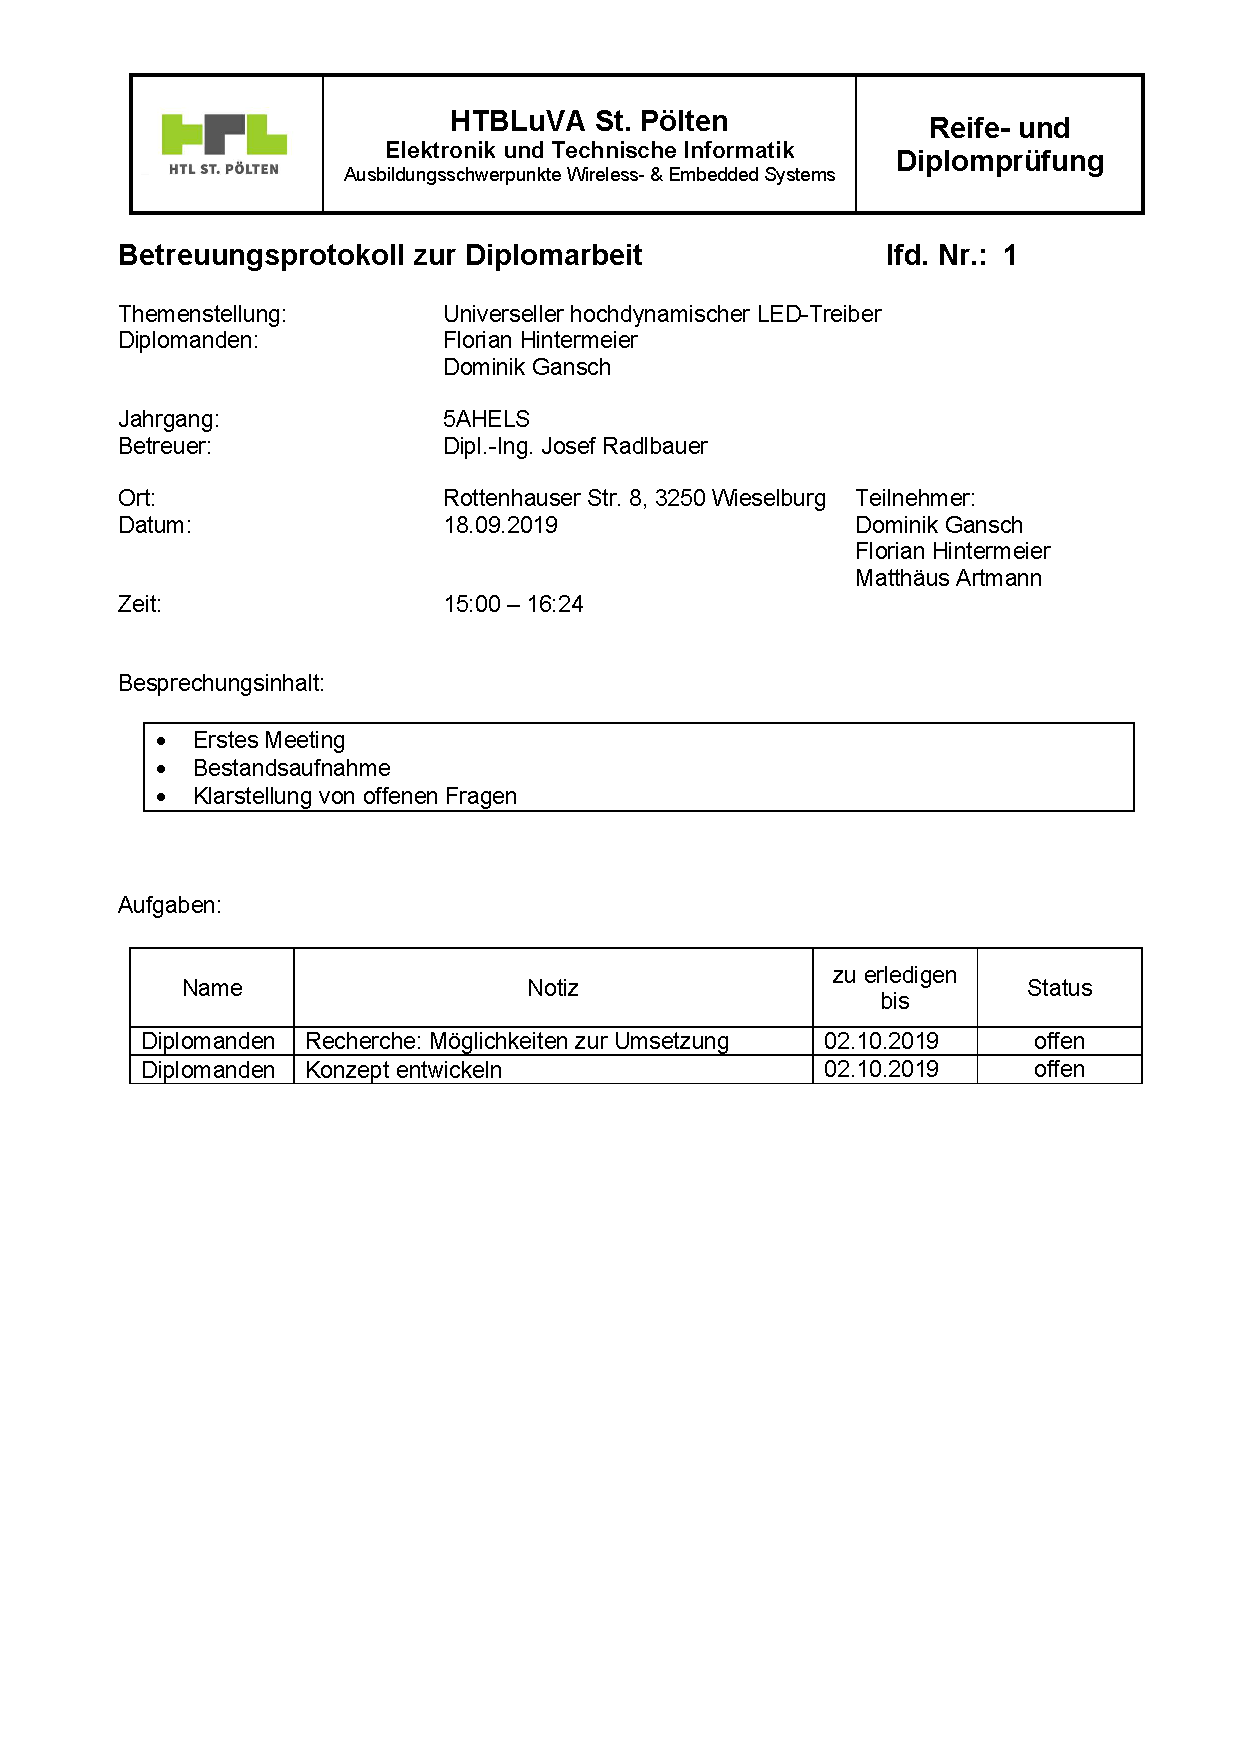
\includepdf[pages=-, scale=0.9,pagecommand={\phantomsection\addcontentsline{toc}{chapter}{Diplomarbeit Seminare}}]{seminare/First_DA_Seminar.pdf}
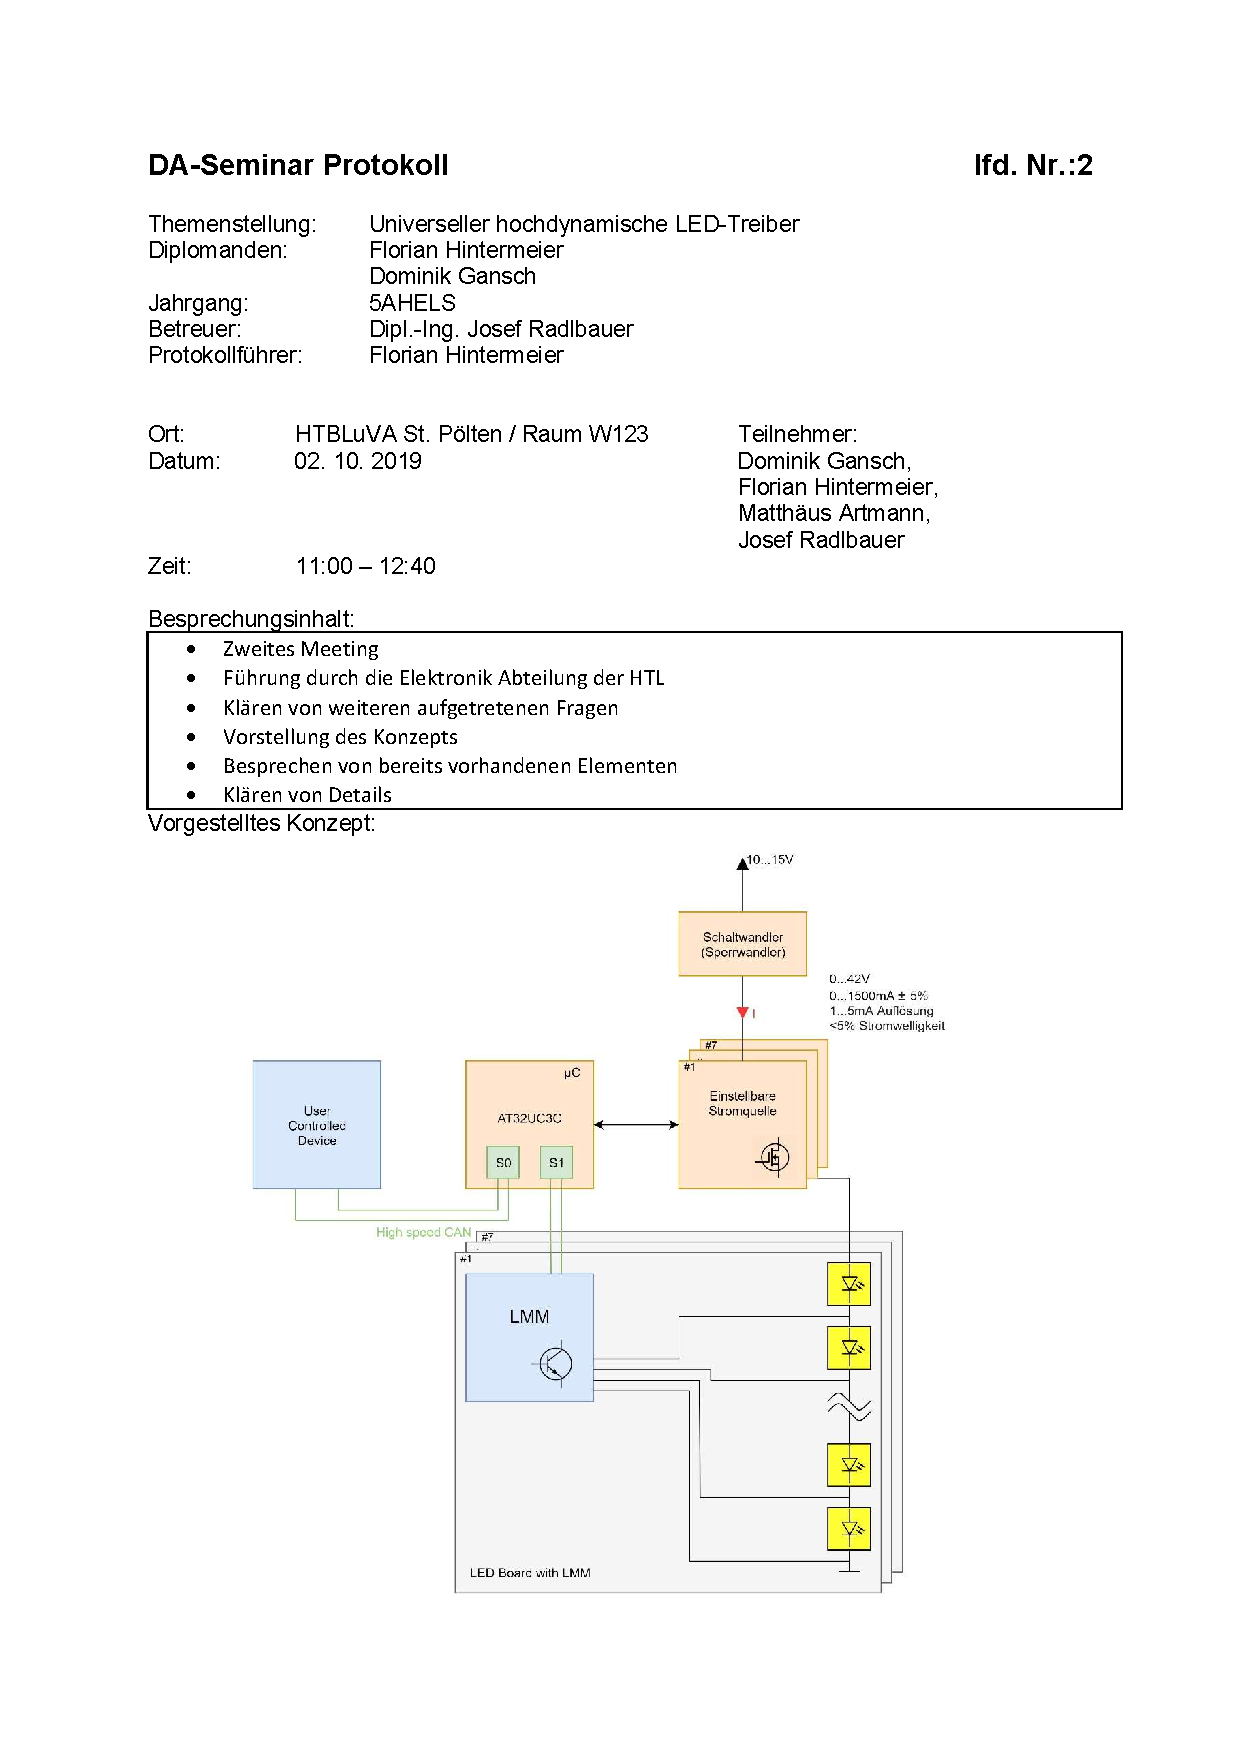
\includepdf[pages=-, scale=0.9, pagecommand={\phantomsection}]{seminare/Second_DA_Seminar.pdf}
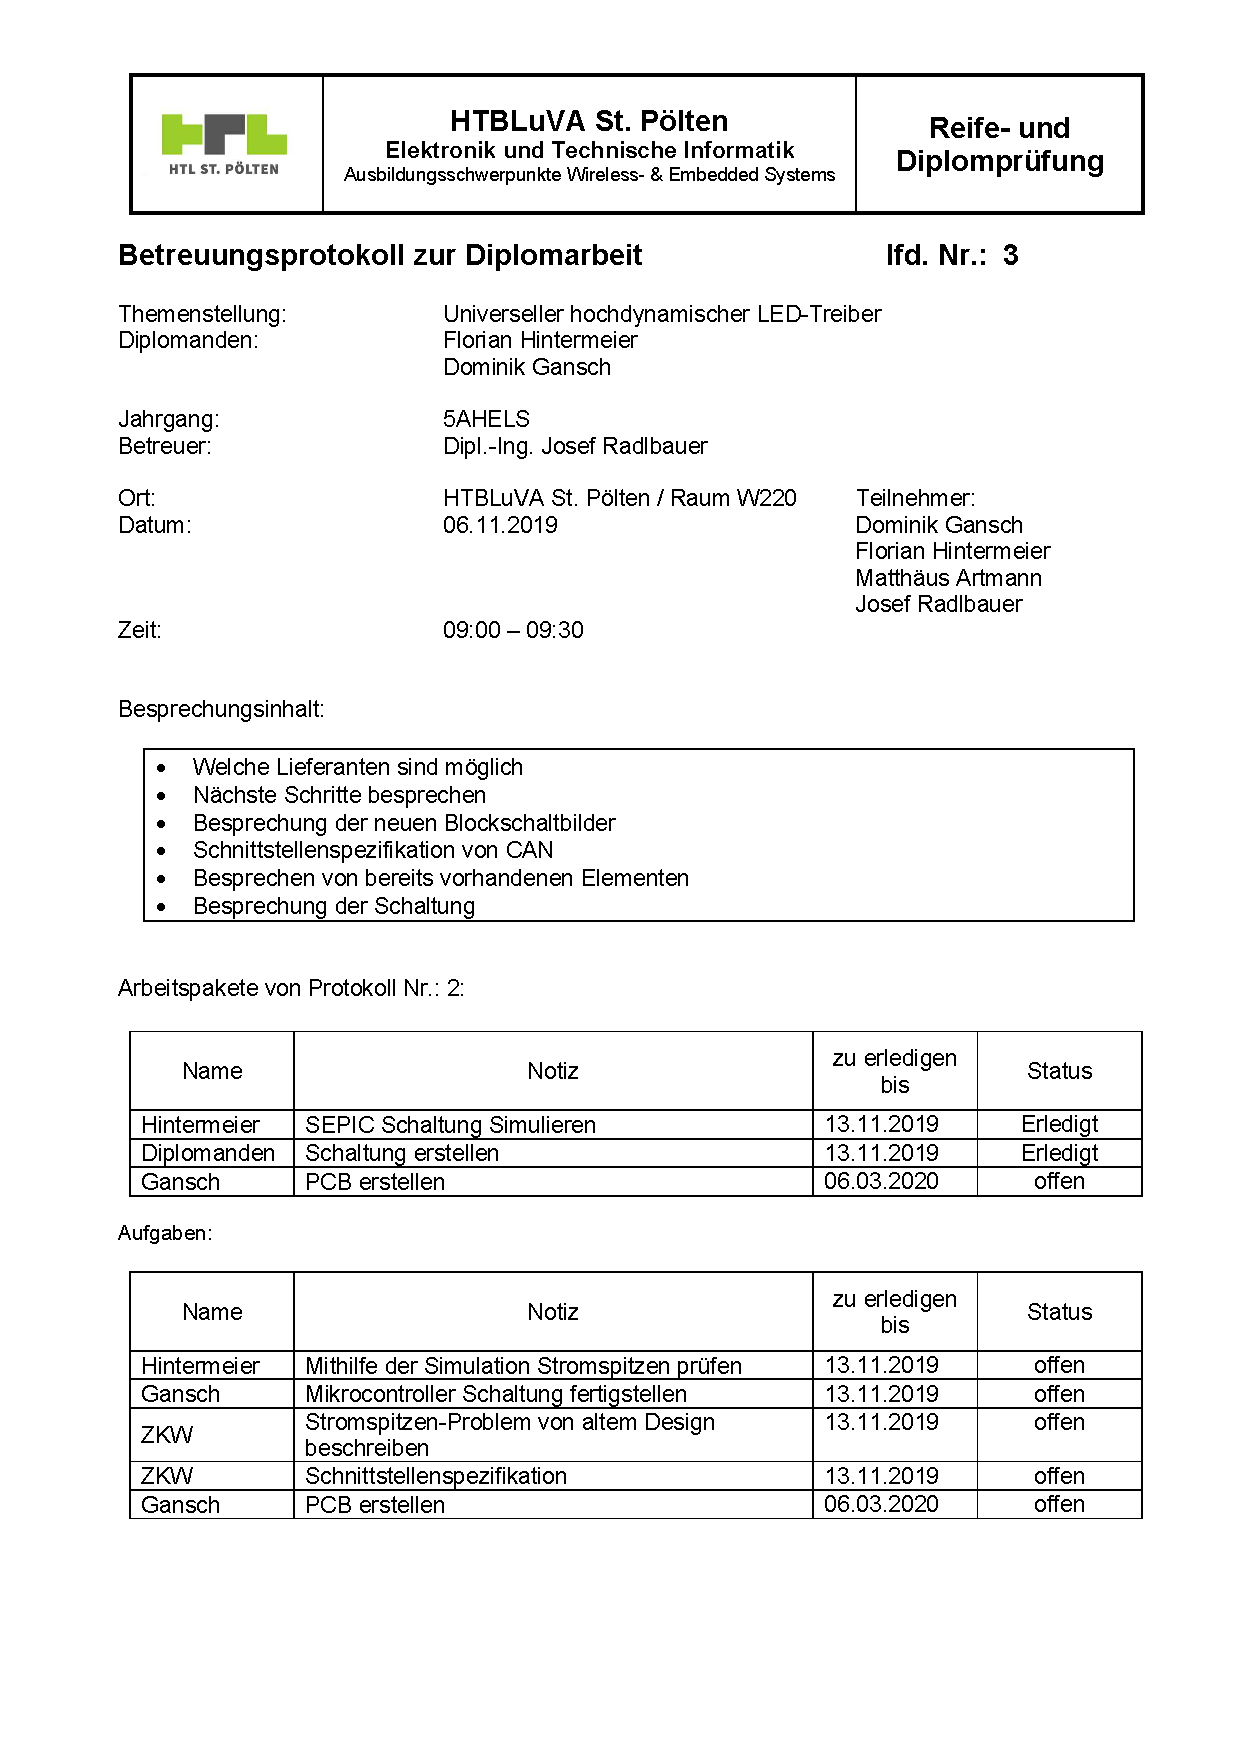
\includepdf[pages=-, scale=0.9, pagecommand={\phantomsection}]{seminare/Third_DA_Seminar.pdf}
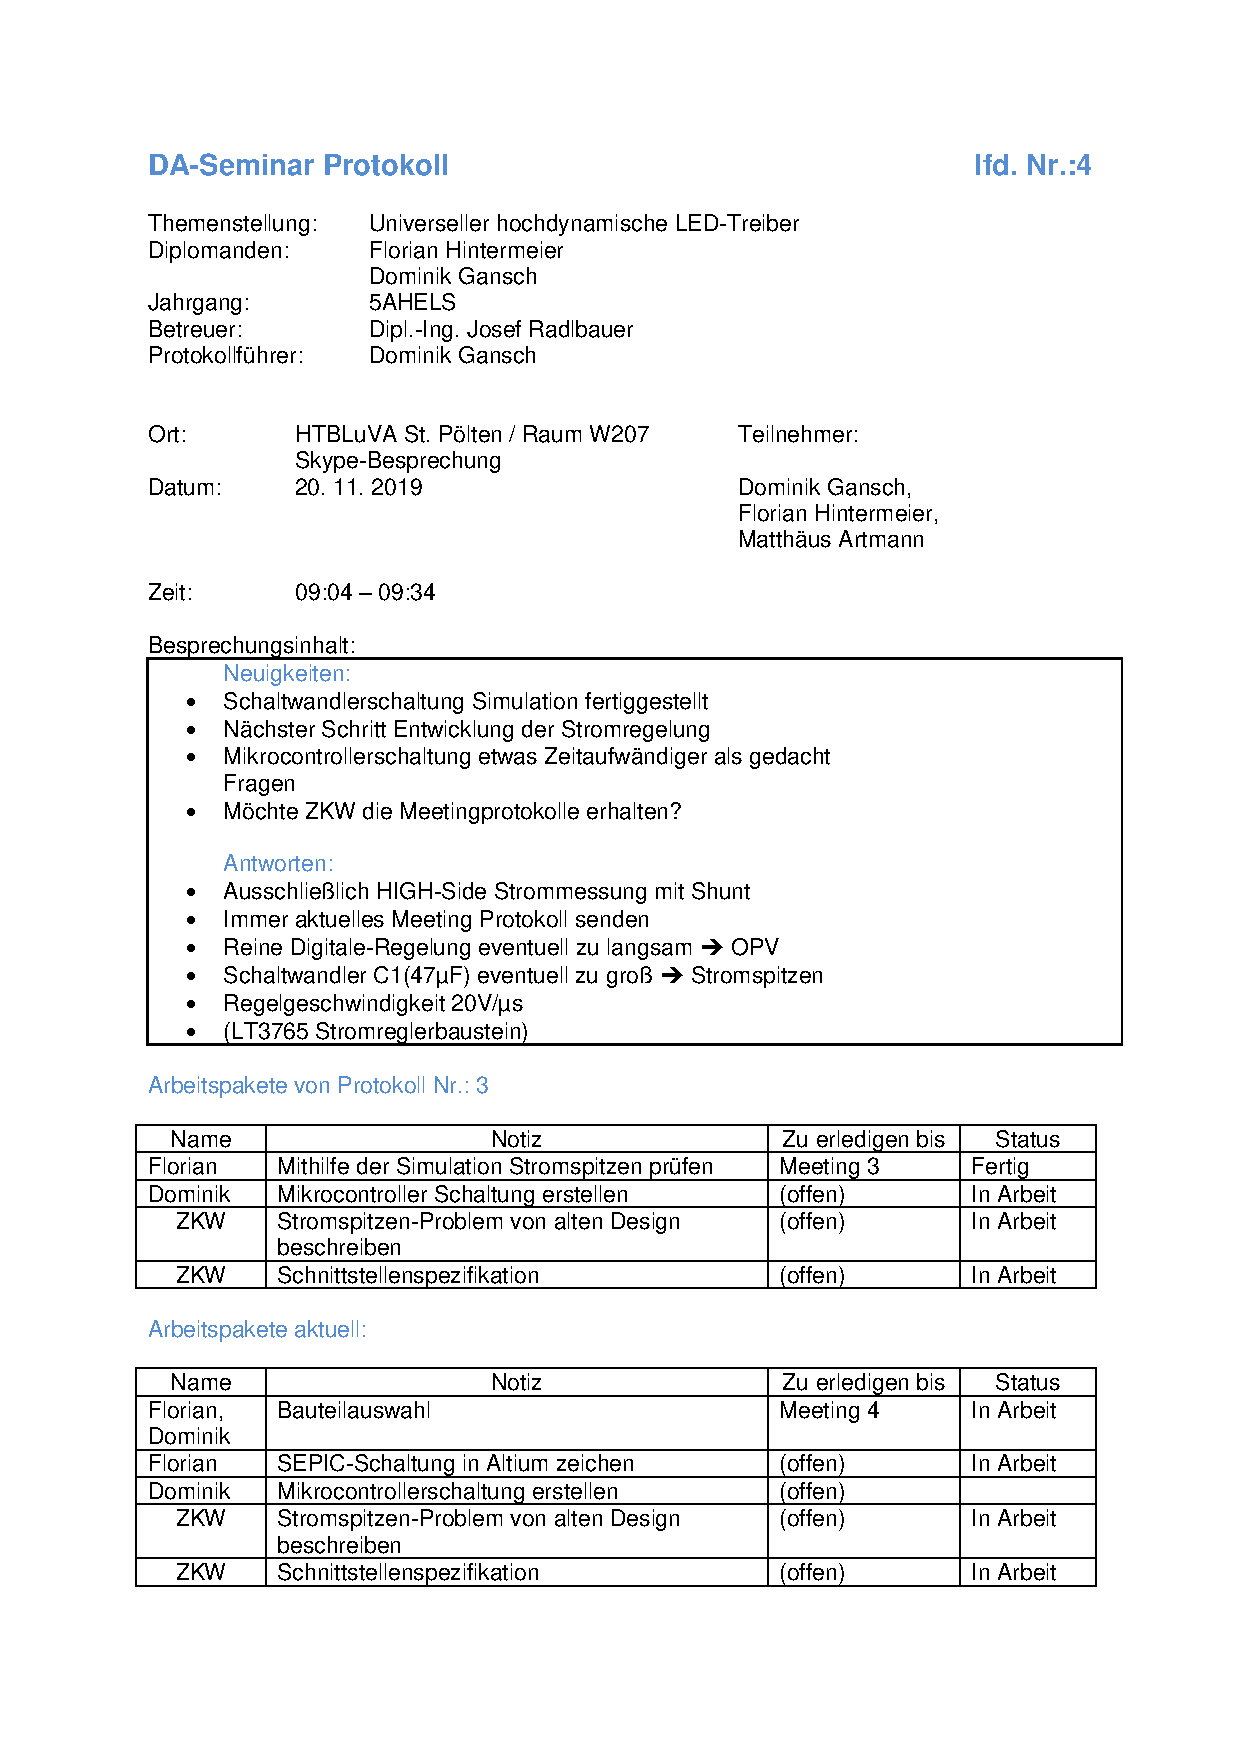
\includepdf[pages=-, scale=0.9, pagecommand={\phantomsection}]{seminare/Fourth_DA_Seminar.pdf}
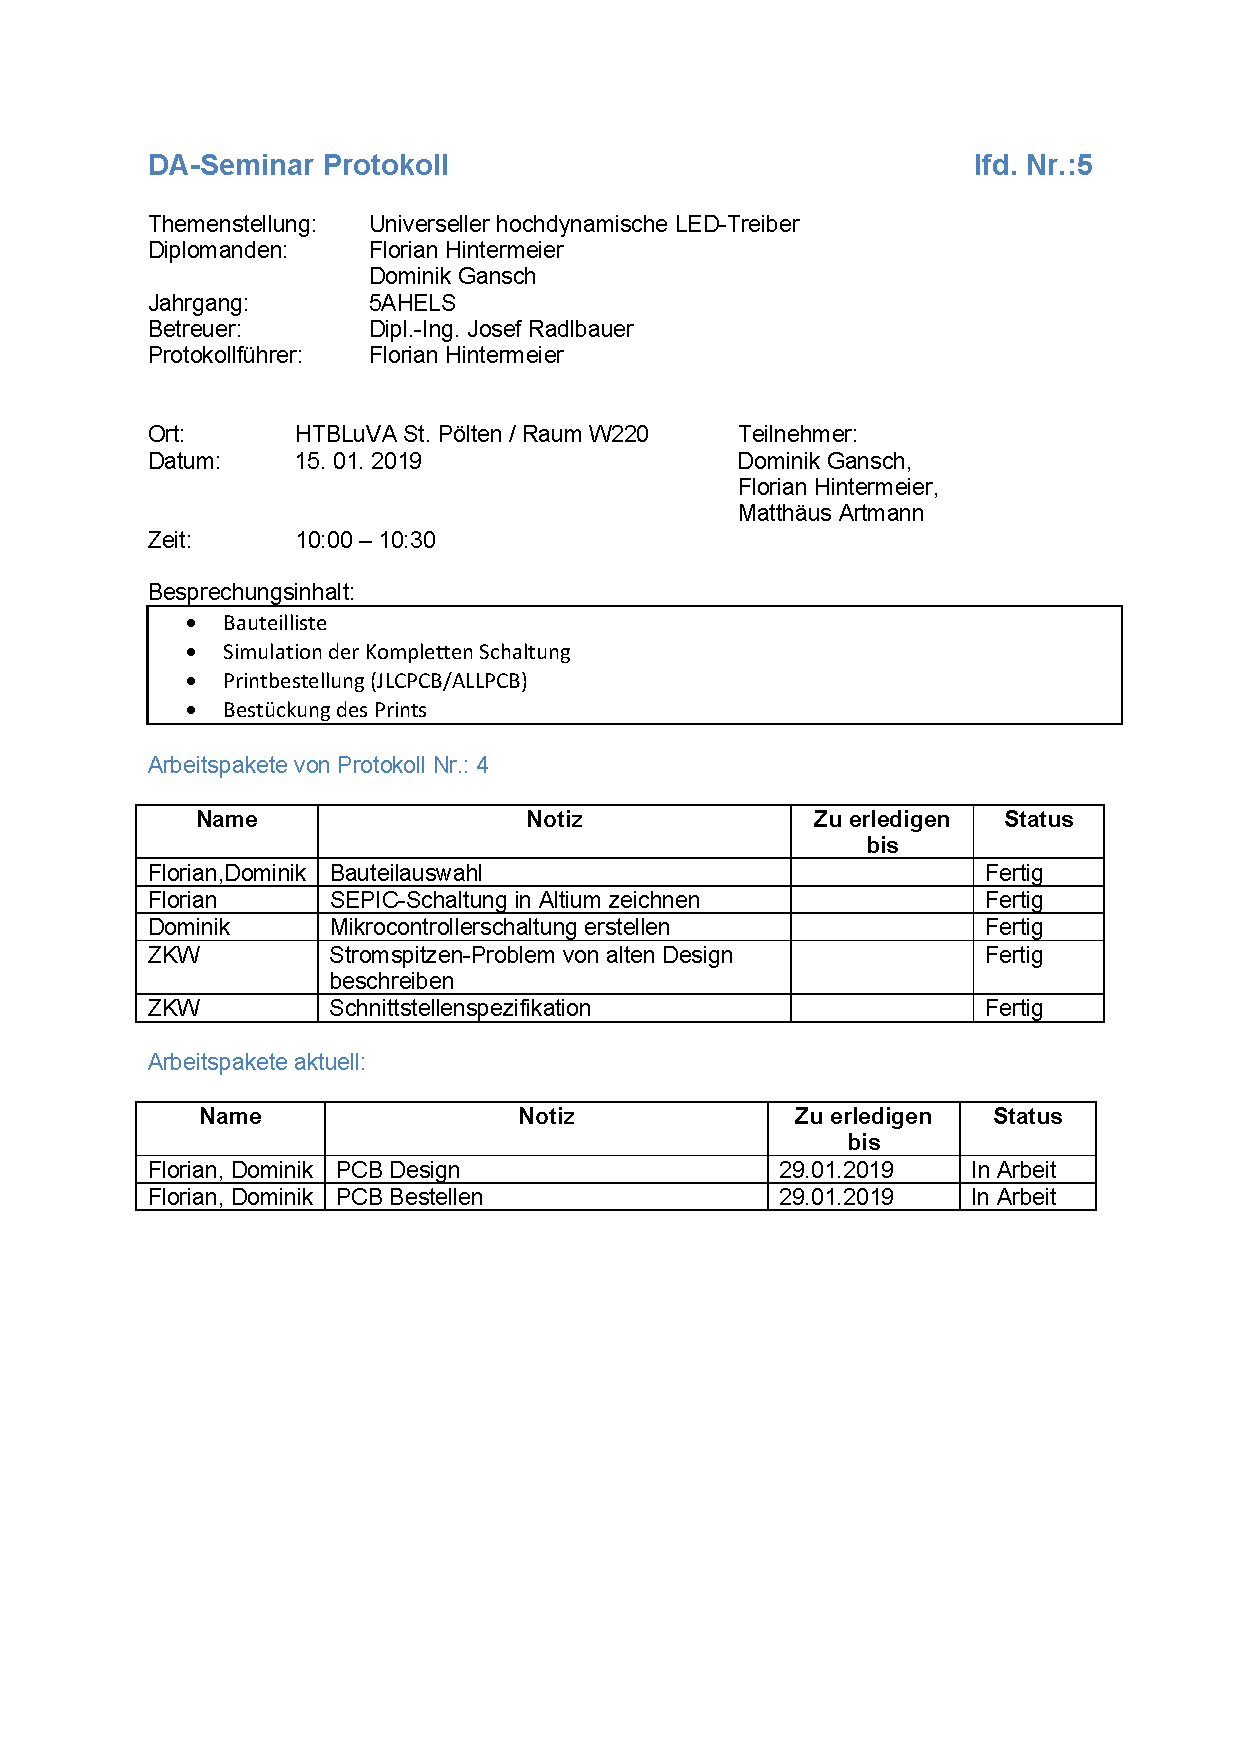
\includepdf[pages=-, scale=0.9, pagecommand={\phantomsection}]{seminare/Fifth_DA_Seminar.pdf}
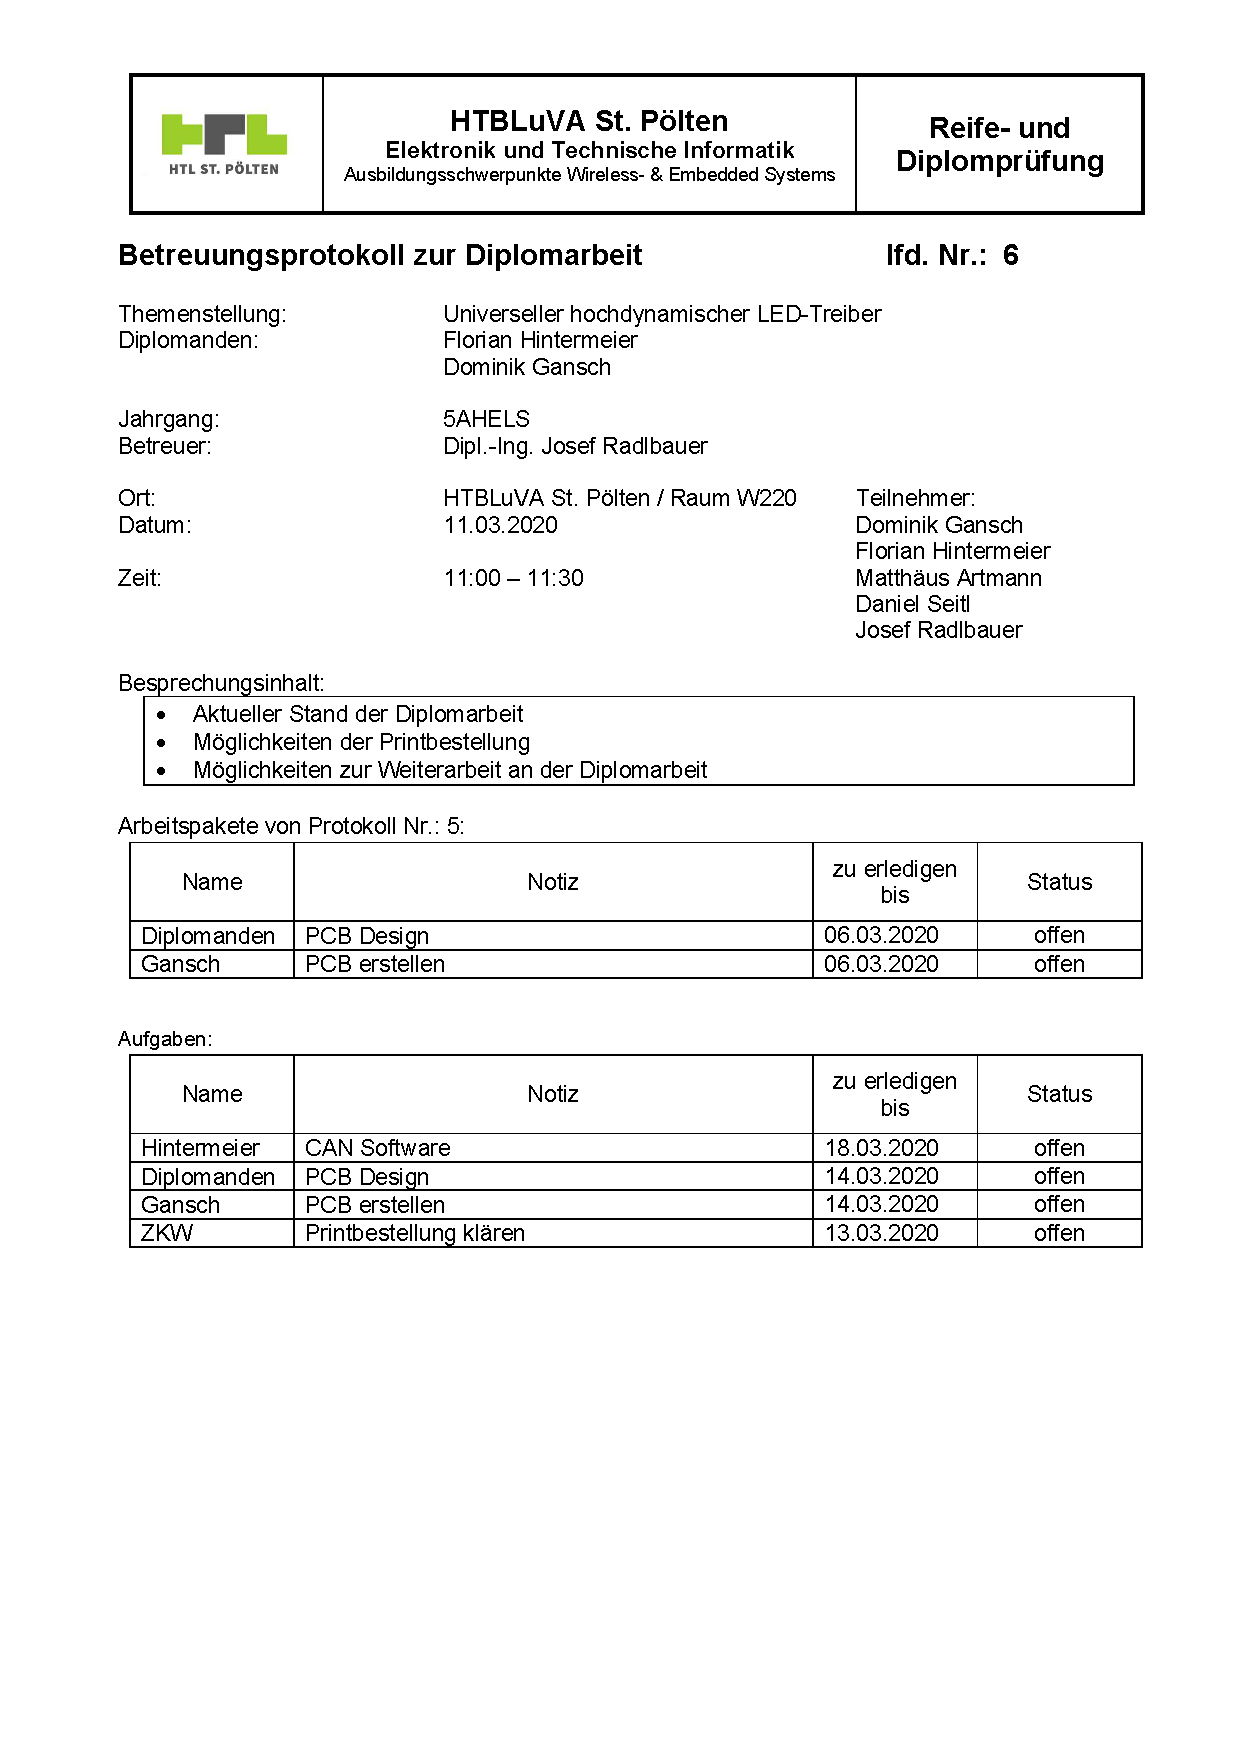
\includepdf[pages=-, scale=0.9, pagecommand={\phantomsection}]{seminare/Sixth_DA_Seminar.pdf}
%%=====================================================%%
\end{document}
